%
% @file projekt-01-kapitoly-chapters.tex
% @author David Kvaček (xkvace00@stud.fit.vutbr.cz)
% @brief Source code of the LaTeX bachelor's thesis content.
% @date 2025-05-13
%

\chapter{Úvod}
\label{introduction}

Cyklistika je stále populárnějším sportem a~volnočasovou aktivitou, které se věnují nejen profesionální sportovci, ale také rekreační jezdci.
Jízda na kole slouží k~dopravě, relaxaci, poznávání nových míst, pravidelnému tréninku, zábavě či závodění.
S~ohledem na dnešní dobu plnou moderních technologií v~podobě chytrých telefonů, různých sportovních aplikací a~lokalizačních zařízení je zaznamenávání osobních výkonů běžnou praxí.
Stanovení tras však hraje neméně důležitou roli, neboť adekvátně naplánované výlety mohou zásadně ovlivnit celé cyklistické zážitky.

Většina existujících řešení se často zaměřuje na rozbor dokončených aktivit.
Analyzování zaznamenaných výkonů je bezesporu klíčové pro pochopení dosažených výsledků a~sledování případných pokroků, nicméně malé množství aplikací se zabývá důkladným plánováním tras před samotnými jízdami a~téměř žádné nepokrývají oblast podrobné vizualizace úseků stoupání.
Stoupání vždy představují náročné segmenty tras, které mohou mít výrazný vliv na předvedené výkony a~potěšení z~jízd.
Jejich předběžné detailní prozkoumání může přispět k~efektivnějšímu rozvržení sil a~přizpůsobení tréninkových plánů individuálním potřebám.

Cílem této práce je zpracovat vybranou problematiku na multiplatformní úrovni a~přinést komplexní řešení, které umožní uživatelům plánovat vyjížďky s~ohledem na osobní preference a~schopnosti, zejména pokud jde o~náročnost terénu.
Díky tomu by měli být cyklisté schopni dosáhnout optimálních výkonů a~zároveň maximalizovat svůj potenciál při každé jízdě, a~to především v~členitém území.

Kapitola \ref{technology-for-analysis-and-visualisation-of-planned-cycle-routes}~představuje masově používané satelitní systémy, které jsou schopné určit přesnou aktuální polohu, jednotlivé datové formáty, způsoby uchování a~reprezentace geografických dat a~přehled aktuálně použitelných řešení, včetně shrnutí současného stavu.
Na tyto základní principy navazuje kapitola \ref{planning-of-sports-activities-according-to-the-difficulty-of-the-marked-goals}, která přibližuje postup vlastního plánování cyklistických výjezdů, dále uvádí definice koeficientů, ze kterých se skládá výsledná objektivní obtížnost.
Analýza a~definice uživatelských požadavků společně s~problémy, které by měla navržená aplikace řešit, se nachází v~kapitole \ref{problem-analysis}.
Kapitola \ref{design-of-the-solution}~obsahuje informace o~návrhu řešení, včetně elementárních funkcionalit aplikace.
Součástí kapitoly \ref{implementation}~je shrnutí nejdůležitějších prvků implementace a~její stručný popis.
V~poslední kapitole \ref{testing}~se nachází průběh a~výsledky testování navržené aplikace při použití reálných vstupních dat.

\chapter{Technologie pro analýzu a~vizualizaci naplánovaných cyklotras}
\label{technology-for-analysis-and-visualisation-of-planned-cycle-routes}

V~současné době jsou moderní technologie nepostradatelnou součástí mnoha oblastí lidského života.
S~rostoucím zájmem o~venkovní sporty a~zejména o~cyklistiku se objevuje potřeba pokročilých nástrojů pro plánování, analýzu a~monitorování tras.
Takové služby mohou cyklistům a~obecně všem sportovcům přispět k~lepšímu porozumění obtížnosti a~časové náročnosti naplánovaných aktivit.

Pro popsané účely je důležitá aktuální poloha, což platí nejen ve sportu obecně, ale především v~cyklistice.
Jízda na kole patří mezi venkovní činnosti a~dostupnost lokalizačních služeb je zásadní jak po stránce statistické s~možností zaznamenávat a~plánovat vlastní trasy, tak i~kvůli bezpečnosti.
Při souběžném využití více satelitních navigačních systémů jsou výsledky měření dostatečně věrohodné a~spolehlivé.

Tyto technologie, které se neustále rozšiřují a~zdokonalují, jsou schopné vypočítat aktuální polohu s~určitou přesností.
Během procesu plánování sportovních aktivit libovolných odvětví zastávají globální satelitní navigační systémy klíčovou roli.

\section{Satelitní navigační systémy}
\label{satellite-navigation-systems}

Pro zajištění přesného určování polohy se moderní technologie opírají o~různé satelitní navigační systémy, které umožňují sledování pohybu v~reálném čase a~v~určité míře zajišťují bezpečnost při venkovních aktivitách.
Uvedené systémy využívají konstelace družic k~pokrytí co největšího území Země a~poskytují spolehlivé údaje nezbytné pro efektivní analýzu a~optimalizaci naplánovaných cyklotras.

Globální družicový polohový systém\footnote{Global Navigation Satellite System (GNSS) --~více viz \url{https://igs.org}.}, často označovaný jako satelitní navigace, nebo někdy také nepřesně jako GPS, se skládá z~konstelace družic.
Obrázek \ref{SystemDifferencesFigure} upřesňuje hlavní rozdíl mezi systémy GNSS a~GPS.
Dílčí družice obíhají kolem Země po specifických trajektoriích s~různorodou dobou oběhu.
Služba díky tomuto konceptu umožňuje vypočítat aktuální polohu na většině území zemského povrchu pomocí matematického postupu trilaterace, jehož zjednodušený princip je na obrázku \ref{TrilaterationFigure}.

\begin{figure}[ht]
    \centering
    \includegraphics[width=0.86\textwidth]{obrazky/1579536824607_637151336203118463.png}
    \caption[]{\textbf{Rozdíl mezi systémy GNSS a~GPS.} Hlavní rozdíl spočívá v~tom, že GNSS označuje souhrnně všechny globální navigační satelitní systémy, zatímco GPS je konkrétní navigační systém provozovaný vládou Spojených států amerických.\footnotemark}
    \label{SystemDifferencesFigure}
\end{figure}

\footnotetext{Převzato z: \url{https://cdn.everythingrf.com/live/1579536824607_637151336203118463.png}.}

\begin{figure}[ht]
    \centering
    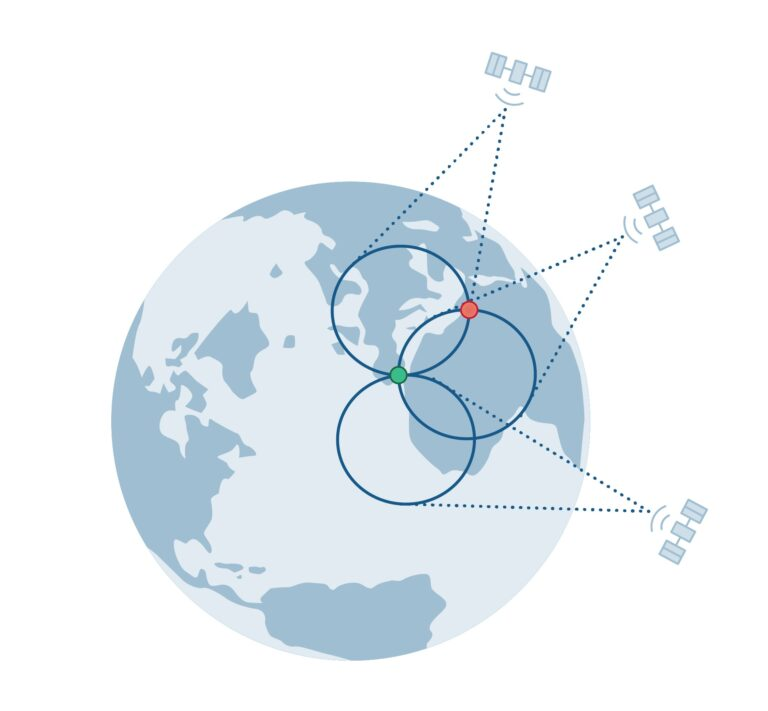
\includegraphics[width=0.52\textwidth]{obrazky/earth-768x711.jpg}
    \caption[]{\textbf{Zjednodušený princip trilaterace.} Metoda sloužící k~určení zeměpisných šířek, zeměpisných délek a~nadmořských výšek (v~reálných aplikacích také času) vyžaduje minimálně tři až čtyři družice, nicméně větší počet satelitů zvyšuje přesnost a~spolehlivost, více viz \cite{SystemsSBG2024}.\footnotemark}
    \label{TrilaterationFigure}
\end{figure}

\footnotetext{Převzato z: \url{https://www.sbg-systems.com/wp-content/uploads/earth-768x711.jpg}.}

Na oběžné dráze Země se vyskytují družice, které se vztahují k~různým konstelacím globálního družicového polohového systému.
Vlády některých zemí poskytují satelitní navigace, které jsou dostupné uživatelům po celém světě.
Mezi nejznámější satelitní navigační systémy patří čínský systém BeiDou, evropský systém Galileo, ruský systém GLONASS nebo americký systém GPS.
Všechny tyto globální družicové satelitní systémy jsou popsané v~následujících podsekcích.

Kromě toho fungují další systémy pouze na regionální úrovni, které zlepšují kvalitu polohových služeb v~rámci obsluhovaných regionů.
Mezi tyto systémy se řadí např. indický IRNSS\footnote{Indian Regional Navigation Satellite System (IRNSS), operačním názvem Navigation with Indian Constellation (NavIC) --~více viz \url{https://www.isro.gov.in}.} nebo japonský QZSS\footnote{Quasi-Zenith Satellite System (QZSS) --~více viz \url{https://qzss.go.jp/en/}.}, které přinášejí vyšší přesnost výpočtů polohy především na asijském kontinentu a~v~Oceánii \cite{NavigationAdvanced2024}.

\subsection{Čínský systém BeiDou}
\label{chinese-beidou-system}

Satelitní navigace BeiDou\footnote{BeiDou Navigation Satellite System (BDS) --~více viz \url{http://en.beidou.gov.cn}.} je autonomní systém vyvíjený Čínskou lidovou republikou.
Služba je schopna pracovat souběžně s~ostatními systémy založenými na principu GNSS a~uživatelé si ve většině případů mohou vybrat, zda si přejí využívat ve svém přijímači rovněž čínskou verzi systému.
Nutno dodat, že při paralelním běhu několika globálních družicových polohových systémů na jediném zařízení se logicky zvyšuje přesnost a~kvalita výpočtů aktuální pozice \cite{KaplanElliottD2017}.

BeiDou má svůj původ v~Čínské lidové republice.
Vývoj systému započal již v~roce 1994, přičemž plného provozu dosáhl v~roce 2020.
Tento systém disponuje přesností v~rozmezí 1,5 až 10 metrů \cite{SpaceFinland2023} a~v~současnosti zahrnuje 35 satelitů \cite{CDDIS2024}.

\subsection{Evropský systém Galileo}
\label{european-galileo-system}

Globální družicový polohový systém Galileo\footnote{European Global Navigation Satellite System (Galileo) --~více viz \url{https://www.gsc-europa.eu}.} je v~současnosti jedinou službou tohoto druhu, která je primárně určena pro komerční účely a~širokou veřejnost.
Na rozdíl od ostatních systémů s~celosvětovým dosahem není výsledkem vývoje jednoho samostatného státu.
Prostředky potřebné pro neustálý chod dodává Evropská unie prostřednictvím Evropské kosmické agentury \cite{KaplanElliottD2017, NurmiJari2014}.

Evropská unie začala vyvíjet svůj navigační systém v~roce 1999.
Plný provoz tohoto systému byl zahájen v~roce 2016.
Satelitní navigace je známá svou vysokou přesností, která se pohybuje mezi 1,5 a~2~metry \cite{SpaceFinland2023}.
Galileo využívá celkem 30 satelitů \cite{CDDIS2024} k~zajištění spolehlivého a~přesného globálního pokrytí.

\subsection{Ruský systém GLONASS}
\label{russian-glonass-system}

Systém GLONASS\footnote{Globalnaja navigacionnaja sputnikovaja sistěma (GLONASS) --~více viz \url{https://glonass-iac.ru}.} je jedním ze čtyř ústředních globálních satelitních navigačních systémů, který od 70. let 20. století postupně implementuje Svaz sovětských socialistických republik, později od roku 1991 Ruská federace.
Služba, nejdříve vymezená výhradně pro vojenské potřeby, se stala přímým konkurentem amerického GPS \cite{KaplanElliottD2017}.

Satelitní navigační systém, původně vyvinutý Svazem sovětských socialistických republik, nyní Ruskou federací, je v~procesu vývoje již od roku 1976.
Plné operační schopnosti tohoto systému bylo docíleno v~roce 2011.
Systém GLONASS je schopen dosáhnout přesnosti v~rozmezí 3~až 5~metrů \cite{SpaceFinland2023}.
Podle nejnovějších údajů funguje v~rámci rozsáhlé sítě 26 satelitů \cite{CDDIS2024}.

\subsection{Americký systém GPS}
\label{american-gps-system}

Globální polohový systém, zkráceně GPS\footnote{Global Positioning System (GPS), původně Navstar GPS -- více viz \url{https://www.gps.gov}.}, původním názvem Navstar GPS, je celosvětově nejvíce rozšířená satelitní navigace.
Tímto produktem disponují Spojené státy americké a~podobně jako systémy BeiDou a~GLONASS byl zpočátku navržený pro vojenskou ochranu.
Momentálně slouží armádě i~civilním uživatelům \cite{MortonYuJ2021}.

Globální polohový systém pochází ze Spojených států amerických, kde byl jeho vývoj zahájen v~roce 1973 \cite{KaplanElliottD2017}.
Po deseti letech intenzivního rozvoje byl systém uveden do plného provozu v~roce 1983.
GPS, složený ze soustavy 24 satelitů \cite{CDDIS2024}, dosahuje přesnosti určování polohy v~rozmezí 2~až 4~metrů \cite{SpaceFinland2023}.

\subsection{Praktické využití satelitních navigačních systémů}

Globální a~regionální družicové polohové systémy v~dnešní době zvládají rozpoznat aktuální polohu GNSS přijímačů s~přesností na jednotky metrů.
Kvalita a~spolehlivost jednotlivých poskytovatelů polohových služeb plynule roste, nicméně s~tím souvisí rovněž vyšší nároky uživatelů.
Velké množství elektronických zařízení má ve svém těle zakomponované specifické čipy, které jsou schopné přijímat a~zpracovat signály z~družic.
V~současnosti se celosvětové pokrytí pohybuje na velmi vysoké úrovni.
Obrázek \ref{ConstellationCombinationsFigure} demonstruje počet viditelných satelitů různých kombinací konstelací.

Vyjma hustě zalesněných oblastí a~míst v~blízkosti vysokých budov se zakrytým výhledem na oblohu lze určit aktuální umístění takřka kdekoliv na světě.
Dnes je využívání těchto služeb pro civilní obyvatelstvo bezplatné a~hraje významnou roli v~každodenním životě.
Pro kvalitní grafickou analýzu a~podrobnou vizualizaci naplánovaných cyklistických tras je nutné znát nejen přesnou polohu v~rámci vybraných aktivit, ale také další důležité detaily o~okolním terénu, které přispívají k~celkovému povědomí ohledně zbývajících úseků stop.

Tyto informace jsou nepostradatelné především v~úsecích stoupání, sloužící k~odpovídajícímu a~realistickému znázornění náročnějších pasáží.
Pro tyto účely jsou geografická data, získaná prostřednictvím globálních družicových polohových systémů, dostupná v~různých formátech, které slouží pro přesný popis krajiny.

\newpage

\begin{figure}[ht]
    \centering
    \includegraphics[width=0.76\textwidth]{obrazky/Number-of-visible-satellites-for-six-different-constellation-combinations-The.png}
    \caption[]{\textbf{Množství viditelných satelitů.} Celkový počet viditelných družic pro šest různých kombinací konstelací. Zkratky GPS, GLO, BDS a~GAL představují satelitní navigační systémy GPS, GLONASS, BeiDou a~Galileo.\footnotemark}
    \label{ConstellationCombinationsFigure}
\end{figure}

\footnotetext{Převzato z: \url{https://www.researchgate.net/profile/Lin-Pan-23/publication/318711986/figure/fig1/AS:614012010119179@1523403279793/Number-of-visible-satellites-for-six-different-constellation-combinations-The.png}.}

\section{Způsoby získávání a~uchovávání geografických dat}
\label{methods-of-obtaining-and-storing-geographic-data}

Pro detailní analýzu a~přehledné zpracování formou grafických vizualizací jsou nezbytná vstupní data, obsahující podrobné informace o~zeměpisných souřadnicích, nadmořských výškách či doplňujících metadatech.
Požadované údaje pro tyto účely lze získat několika způsoby.
První a~současně nejjednodušší možností je naplánování vlastních cyklistických tras prostřednictvím vhodných portálů s~mapovými podklady.
Vygenerované soubory se všemi podstatnými záznamy mohou následně sloužit jako vstupní data během procesu plánování vlastních tréninkových výkonů.

Další dostupnou metodou je využití osobních soukromých dat, získaných absolvováním sportovních aktivit, v~podobě specifických formátů souborů.
Zaznamenat výkony, včetně množství údajů kritických pro potřeby analýzy a~grafického znázornění, je momentálně daleko snazší než v~minulosti.
Dnes již není nutné vlastnit speciálně určené přístroje se zabudovanými čipy, moduly a~specifickými senzory, ale bohatě postačí mobilní telefony s~nainstalovanými sportovními aplikacemi.
Sekce \ref{current-solutions-for-analysis-and-visualisation-of-planned-routes}~blíže popisuje existující řešení zadaného problému, z~nichž většina má k~dispozici mobilní verze svých systémů, které umožňují pohotově zaznamenat sportovní výkony.

V~neposlední řadě je možné získat geografická data stažením odpovídajících, volně přístupných, souborů z~internetu, nicméně tento způsob není ideální, protože na geodata se mohou vztahovat autorská práva, soubory mohou být poškozené, nebo nemusí obsahovat kompletní informace.
Bez ohledu na zvolenou variantu jsou vstupní data součástí souborů typických formátů, které mají charakteristické vlastnosti.
Mezi nejrozšířenější a~nejvíce používané typy souborů s~geografickými daty v~oblasti cyklistiky patří např. protokol FIT, formát GPX, druh souborů KML a~standard TCX.

\subsection{Formát souboru FIT}
\label{the-fit-file-format}

Standard FIT\footnote{Flexible and Interoperable Data Transfer (FIT) --~více viz \url{https://developer.garmin.com/fit/protocol/}.} je protokol určený výhradně pro soubory s~geografickými údaji, které pocházejí ze sportovních, fitness a~zdravotních zařízení.
Z~dokumentace \cite{Garmin2024} vyplývá, že tento typ souboru je navržen tak, aby měl kompaktní velikost, byl schopný rozšiřitelnosti a~kooperace s~jinými platformami.

Soubory tohoto formátu obsahují zprávy v~podobě jednotlivých záznamů, rozdělených na záhlaví s~definicí a~hlavní tělo s~datově vyplněnými poli \cite{Garmin2024}.
Obrázek \ref{FITProtocol} ilustruje uspořádání elementárních prvků na nejvyšší úrovni.

Soubory aktivit se ve formátu FIT skládají ze tří hlavních částí.
První složkou je hlavička \texttt{File Header} o~velikosti 14 bytů, která nese libovolná metadata vlastních souborů.
Další součástí jsou jednotlivé datové záznamy \texttt{Record}, které ve svém záhlaví \texttt{Record Header} uchovávají informace o~definici a~typu zprávy, zatímco v~samotném hlavním těle \texttt{Record Content} se nachází údaje např. o~tepové frekvenci, kadenci šlapání, ujeté vzdálenosti, nadmořské výšce nebo aktuální rychlosti.
V~neposlední řadě standard obsahuje vlastní vývojová data a~kontrolní součet \texttt{CRC}\footnote{Cyclic redundancy check (CRC) --~více viz \url{https://www.sciencedirect.com/topics/engineering/cyclic-redundancy-check}.}.

Ačkoliv je formát FIT přímo určený pro uchovávání dat sportovních aktivit, na své poměry má malou velikost, může být rozšířen o~další atributy a~elementy podle aktuálního druhu záznamu, k~použití v~rámci procesu plánování cyklistických tras se zdá být příliš robustní.
V~případě potřeby je však možné převést soubor do formátu GPX popsaného níže.

\newpage

\begin{figure}[ht]
    \centering
    \includegraphics[width=0.64\textwidth]{obrazky/fitprotocol_figure14.png}
    \caption[]{\textbf{Formát souboru FIT.} Základní komponenty souboru protokolu FIT, včetně jednotlivých záznamů s~definicí v~hlavičce a~datově vyplněnými poli v~hlavním těle.\footnotemark}
    \label{FITProtocol}
\end{figure}

\footnotetext{Převzato z: \url{https://developer.garmin.com/fit/resources/fitprotocol_figure14.png}.}

\subsection{Formát souboru GPX}
\label{the-gpx-file-format}

GPS eXchange Format\footnote{GPS eXchange Format (GPX) --~více viz \url{https://www.topografix.com/gpx.asp}.} je nejrozšířenější a~zároveň nejvíce používaný typ souboru pro ukládání a~šíření geografických dat.
Formát GPX je založený na jazyku XML\footnote{eXtensible Markup Language (XML) --~více viz \url{https://www.xml.com}.} a~definuje sadu značek pro jednoznačný popis uchovávaných geodat.
Díky tomu, že jsou soubory ve struktuře XML, je jejich schopnost kompatibility a~přenositelnosti značná a~umožňuje snadnou kooperaci mezi zařízeními, které pracují s~geografickými informacemi \cite{TopoGrafix2023}.

Kompozice souborů odpovídá obvyklým normám XML.
Za povinnou hlavičkou, která udává verzi a~kódování, se nachází párový kořenový element \texttt{<gpx>} s~upřesňujícími údaji o~jmenném prostoru, verzí schématu a~původního tvůrce, nejčastěji webových služeb.
Před samotnou evidencí naplánovaných cyklotras se může vyskytovat nepovinný párový element \texttt{<metadata>} pro výčet doplňujících podrobností, jako je autor nebo datum a~čas vytvoření \cite{TopoGrafix2023}.

Formát GPX podporuje pro popis stop tři odlišné elementy, které mohou být v~souborech libovolně kombinovány a~jejich počet není nijak omezen.
Vedle \texttt{<wpt>}\footnote{Waypoint (\texttt{<wpt>}) --~vyjádření jediného místa, či bodu se zeměpisnými souřadnicemi na mapě.} a~\texttt{<rte>}\footnote{Route (\texttt{<rte>}) --~vyjádření seznamu míst, či bodů trasy, směřujících od startu do cíle.} je dostupným typem \texttt{<trk>}\footnote{Track (\texttt{<trk>}) --~vyjádření seznamu míst, či bodů stopy, směřujících od začátku do konce.}, určený pro popis vlastních stop.
Volitelně je v~elementu \texttt{<name>} uveden název a~nedílnou součástí jsou v~prvku \texttt{<trkseg>}, představujícího segmenty tras, konkrétní body \texttt{<trkpt>} s~povinnými atributy \texttt{lat} a~\texttt{lon}, označující zeměpisné šířky a~délky.
Prvky \texttt{<ele>} nebo \texttt{<time>} pro záznamy nadmořských výšek a~časových razítek jsou nepovinné \cite{TopoGrafix2023}.
Příklad záznamu krátké naplánované stopy ve formátu GPX znázorňuje výpis v~příloze \ref{TheGPXFileSample}.

Soubory ve formátu GPX mají textový obsah a~jsou lehce čitelné díky své uspořádanosti a~přehlednosti.
Jelikož se jedná o~tzv. otevřený formát, za jeho použití nejsou uživatelé nuceni platit žádné licenční poplatky.

\subsection{Formát souboru KML}
\label{the-kml-file-format}

KML\footnote{Keyhole Markup Language (KML) --~více viz \url{https://pro.arcgis.com/en/pro-app/latest/help/data/kml/what-is-kml-.htm}.} je, podobně jako GPX, formát souboru se strukturou založenou na jazyku XML.
Soubory tohoto typu mají schopnost sdílet a~zobrazovat informace v~geografickém kontextu, které mohou být vykreslovány nebo vizualizovány v~prohlížečích systému Earth\footnote{Google Earth --~více viz \url{https://www.google.com/earth/about/}.} \cite{ConsortiumOpenGeospatial2024}.
Vnitřní skladba souboru ve formátu KML se významně podobá typu GPX.

Pro porovnání se ve výpisu přílohy \ref{TheKMLFileSample} nachází velmi podobná stopa, jako v~případě souboru GPX, tentokrát však ve formátu KML.
Při konfrontaci těchto dvou protokolů je zřetelné, že pro plánování cyklotras a~jejich detailní grafické analýzy a~vizualizace je daleko přijatelnější formát GPX.

Typ souboru GPX je zaměřený na jednoduchost a~přehlednost.
Základními prvky jsou body trasy s~přesnými zeměpisnými souřadnicemi a~nadmořskými výškami.
Tento formát je široce podporován v~různých aplikacích zaměřených na outdoorové aktivity.

Na druhé straně formát KML nabízí širší možnosti popisu a~zobrazení tras.
Lze využít pohled na trasy z~několika úhlů při různé vzdálenosti od kamery.
Tyto pokročilé vizualizační schopnosti mohou být užitečné pro prezentaci a~sdílení naplánovaných stop, nicméně soubory KML podporují pouze aplikace a~prohlížeče, které jsou založené na systému Earth.

\subsection{Formát souboru TCX}
\label{the-tcx-file-format}

TCX\footnote{Training Center XML (TCX) --~více viz \url{https://www.earlyinnovations.com/gpsphotolinker/about-gpx-and-tcx-file-formats.html}.} je formát pro výměnu dat od společnosti Garmin.
Tento typ souboru má analogickou strukturu jako předchozí zmíněné protokoly GPX a~KML, ale s~naplánovanými trasami pracuje mírně odlišně a~počítá s~tím, že se jedná o~sportovní aktivity, nikoliv pouze o~posloupnosti jednotlivých míst, či bodů v~rámci stopy na mapě.
Formát TCX navíc poskytuje podporu přenosu pro údaje např. o~kadenci jízdy na kole, tepové frekvenci nebo počtu spálených kalorií \cite{AnssensCharles2021}.

Datové soubory tohoto typu jsou rovněž vhodné pro navigaci po předem naplánovaných stopách.
Výpis v~příloze \ref{TheTCXFileSample} ilustruje jednoduchou cyklotrasu se stejným startem, průběhem i~cílem jako v~předchozích případech.
Z~ukázky plyne, že formát TCX je zdaleka nejpropracovanější.

Protokol TCX představuje další možnou variantu výměny a~sdílení geografických dat mezi různými zařízeními.
Na soubory typu TCX se podle dostupných informací nevztahují žádná licenční omezení, díky struktuře XML je obsah čitelný a~zaznamenané údaje je možné jednoduše upravovat \cite{AnssensCharles2021}.
Zahrnuty jsou nejdůležitější informace pro detailní analýzu a~vizualizaci cyklistických tras, mezi které se řadí zeměpisné souřadnice a~nadmořské výšky každého bodu stopy.
I~když se na první pohled může zdát, že je formát TCX zbytečně komplexní, stále reprezentuje odpovídající alternativu k~souborům typu GPX.

\section{Dostupná geografická data vhodná pro analýzu cyklotras}
\label{available-geographic-data-suitable-for-cycle-routes-analysis}

Tvorba analýzy a~pokročilé grafické prezentace naplánovaných cyklistických tras vyžaduje relevantní a~pokud možno anonymizované zdroje geografických dat.
Tyto nepostradatelné informace o~zeměpisných souřadnicích či nadmořských výškách jsou obsahem výše popsaných souborů různých datových formátů, které jsou vhodné pro různé typy aktivit.
Samotná geodata jsou výsledkem dlouhodobého měření a~výpočtů satelitních navigačních služeb.
Obecně lze uvést několik odlišných způsobů, jak získat požadovaná vstupní data, která se ve větší míře používají pro ekvivalentní rozbory.
Pro účely této práce jsou uvedené techniky rozdělené na dva přístupy.

Jedna metoda spočívá ve využívání tzv. primárních zdrojů, tedy dat, která pocházejí přímo z~vlastního fondu.
Jednoduše řečeno se jedná o~data, která jsou výsledkem měření prostřednictvím určitých GPS přístrojů vlastněných uživateli \cite{KlufovaRenata2016}.
Zaznamenané podklady, dostupné v~jednom z~dříve popsaných formátů, je následně možné aplikovat pro potřeby analýzy.

Již z~principu fungování osobního měření zaručuje tento postup plnou anonymitu.
Naměřené údaje zahrnují chyby vzniklé pouze v~závislosti na přesnosti, spolehlivosti a~kvalitě daných zařízení.
Na druhé straně je nutné vynaložit úsilí a~prostředky pro individuální zaznamenání sportovních výkonů.
Trasy určené k~analýze je navíc nezbytné absolvovat osobně a~poté exportovat geografická data do datových souborů ve zvolených formátech.

Patřičnou alternativou jsou sekundární zdroje dat, mezi které se řadí již existující otevřené mapové sady a~geografické podklady \cite{KlufovaRenata2016}.
Na tento fenomén se v~dnešní době zaměřuje nemalé množství různých aplikací a~portálů, jmenovitě se jedná např. o~plánovač tras Komoot, mapový portál Mapy.cz, cyklistická navigace Ride with GPS či internetová služba Strava.
Skrze vybrané aplikace jsou uživatelé schopni naplánovat vlastní cyklistické stopy, které vyexportují do souborů v~požadovaných formátech a~ty mohou sloužit jako vstupní data pro analýzu se všemi nezbytnými údaji, včetně zeměpisných souřadnic i~nadmořských výšek.

Stejně jako první způsob, i~druhá možnost získávání geografických dat nabízí jejich poskytování anonymně.
Detailní údaje o~naplánovaných cyklotrasách obsahují chyby měření minimálně ve stejné míře jako data primární.
Pro účely analytického zpracování však není nutné investovat žádnou námahu ani prostředky.
Veškerá vstupní data s~geografickými informacemi se nachází v~exportovaných souborech zvolených formátů, které jsou vhodné pro budoucí analýzy.

\section{Metody vizualizace dat cyklistických tras}
\label{cycle-route-data-visualisation-methods}

Surová geografická data zdrojových souborů v~podobě množství jedniček a~nul jsou v~podstatě nečitelná a~nemají žádnou vypovídající hodnotu.
Jednotlivé aspekty každé předem naplánované jízdy lze prezentovat několika různými pohledy.
Existují dostupné nástroje a~metody, díky kterým se vstupní geografická data mohou transformovat na přehlednější, výrazně jednodušší a~relevantní grafická znázornění.
Takové konkrétní podoby zobrazení dat o~cyklotrasách mají pro uživatele mnohem větší informační hodnotu.

Detailní vizualizace náročných pasáží stoupání umožňují sportovcům lépe pochopit průběh a~obtížnost aktivit.
Předběžné analýzy poskytují cyklistům příležitost zvolit vhodné tempo, rychlost a~vynaložené úsilí během kritických úseků tras.
Reprezentace vstupních dat různými vizualizačními metodami pomocí podrobných grafů, schematických ilustrací nebo mapových zobrazení je daleko efektivnější a~srozumitelnější.

Pro každou metriku a~rozdílné informace o~naplánovaných stopách jsou vhodné specifické metody grafických znázornění.
Není možné zobrazit zeměpisné souřadnice a~výšková data s~údaji o~nadmořských výškách totožným způsobem.
Zeměpisné šířky a~zeměpisné délky jednotlivých bodů v~rámci trasy je žádoucí vizualizovat jako propojené linie těchto míst na mapových podkladech.
Naopak k~vyjádření průběhu nadmořských výšek jsou odpovídajícími výstupy spojnicové nebo sloupcové grafy doplněné o~další podrobnosti v~podobě vzdálenosti či sklonu stoupání \cite{BruggerAnnina2017}.
Samotný proces plánování by měl být usnadněn díky populárním a~oblíbeným trasám v~dané oblasti, které jsou nejčastěji zobrazeny technikou heat map, více viz \cite{PokojskiWojciech2021}.

\subsection{Zobrazení zeměpisných souřadnic trasy}
\label{display-the-geographical-coordinates-of-the-route}

Naplánované cyklistické trasy se skládají z~posloupnosti bodů, přičemž každé takové místo má své zeměpisné souřadnice.
Existuje jistě mnoho způsobů, kterými lze uživateli detailně představit přesný průběh takto vytvořených stop, nicméně zobrazení barevné linie na mapových podkladech propojující sekvenci míst s~určitými zeměpisnými šířkami a~délkami poskytuje efektivní přehled o~kompletních aktivitách.
Příklad krátké trasy naplánované prostřednictvím mapového portálu Mapy.cz ilustruje obrázek \ref{RouteCourse}.

Taková interpretace přináší sportovcům zevrubný pohled na tréninky jako celky.
Z~map je však rovněž možné rozpoznat drobné aspekty, jako jsou nebezpečné zatáčky, vzhled krajiny nebo přítomnost přírodních památek, restaurací, vyhlídek či dalších zajímavostí v~bezprostřední blízkosti trasy.
Tyto doplňující poznatky mohou ovlivnit nejen vlastní výkony, ale také celkovou atraktivitu naplánovaných tras.

V~dnešní době je k~dispozici poměrně široké spektrum specializovaných druhů map, mezi které patří i~cykloturistické.
Barevné linie znázorňující stopu ve spojení s~vhodně zvolenými mapovými podklady se zdají být dostatečně uspokojujícím zobrazením celého průběhu aktivit.
Tohoto cíle by nemohlo být dosaženo interpretací založené pouze na množství čísel \cite{KlufovaRenata2016}, které by většina uživatelů nijak nevyužila.

\newpage

\begin{figure}[ht]
    \centering
    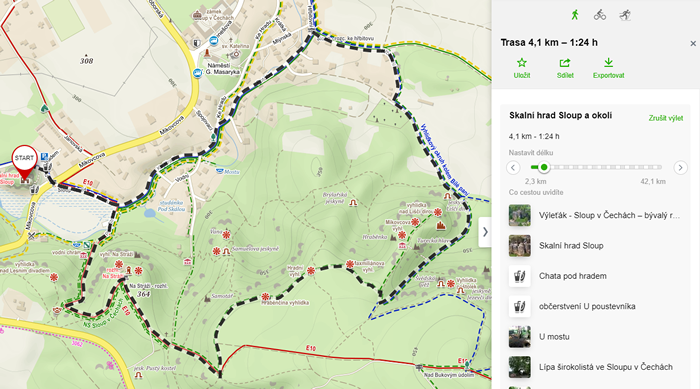
\includegraphics[width=0.86\textwidth]{obrazky/vylet2a.png}
    \caption[]{\textbf{Zobrazení průběhu trasy.} Přesný průběh naplánované trasy na mapovém podkladu vytvořený barevnou linií, která spojuje jednotlivé body polohy.\footnotemark}
    \label{RouteCourse}
\end{figure}

\footnotetext{Převzato z: \url{https://napoveda.seznam.cz/soubory/Mapy/Planovani/vylet2a.png}.}

\subsection{Zobrazení výškového profilu trasy a~stoupání}
\label{display-the-elevation-profile-of-the-route-and-climbs}

Nadmořské výšky hrají významnou roli v~obtížnosti a~časové náročnosti plánovaných výletů.
Je pochopitelné, že rovinaté okruhy bez větších stoupání jsou výrazně jednodušší než vysokohorské etapy s~několika těžkými kopci.
Nejen kvůli těmto obdobným znalostem jsou výškové profily nedílnou součástí podrobné analýzy.
Díky tomu jsou uživatelé schopni alespoň částečně předpovědět obtížnost naplánovaných tras.

Výškové profily je možné vizualizovat spojnicovými grafy, které propojují nadmořské výšky míst v~rámci cyklotrasy.
Tyto grafické výstupy přehledně zobrazují průběhy rovinatých pasáží, úseků stoupání i~klesání celé aktivity.
Na obrázku \ref{RouteElevationProfile} je zjednodušený výškový profil naplánované trasy, který nabízí mapový portál Mapy.cz.

Další možnou interpretací výškových dat relevantní pro tuto práci jsou sloupcové grafy, prezentující průběh jednotlivých úseků stoupání během aktivit.
Analogické diagramy mají momentálně největší potenciál a~prostor k~dalšímu zdokonalování.
V~současnosti je většina těchto vizualizací statická, ale sportovci i~rekreační cyklisté by jistě ocenili podrobné zobrazení výškových profilů stoupání.
Ukázka vývoje nadmořských výšek náročného segmentu popsaným grafem se nachází na obrázku \ref{ClimbElevationProfile}.

\newpage

\begin{figure}[ht]
    \centering
    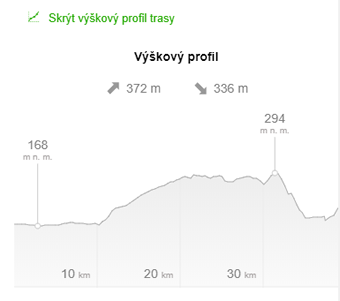
\includegraphics[width=0.64\textwidth]{obrazky/planovani-vyskovy-profil.png}
    \caption[]{\textbf{Zobrazení výškového profilu trasy.} Vizualizace výškového profilu celé naplánované trasy spojnicovým grafem.\footnotemark}
    \label{RouteElevationProfile}
\end{figure}

\footnotetext{Převzato z: \url{https://napoveda.seznam.cz/soubory/Mapy/Planovani/planovani-vyskovy-profil.png}.}

\begin{figure}[ht]
    \centering
    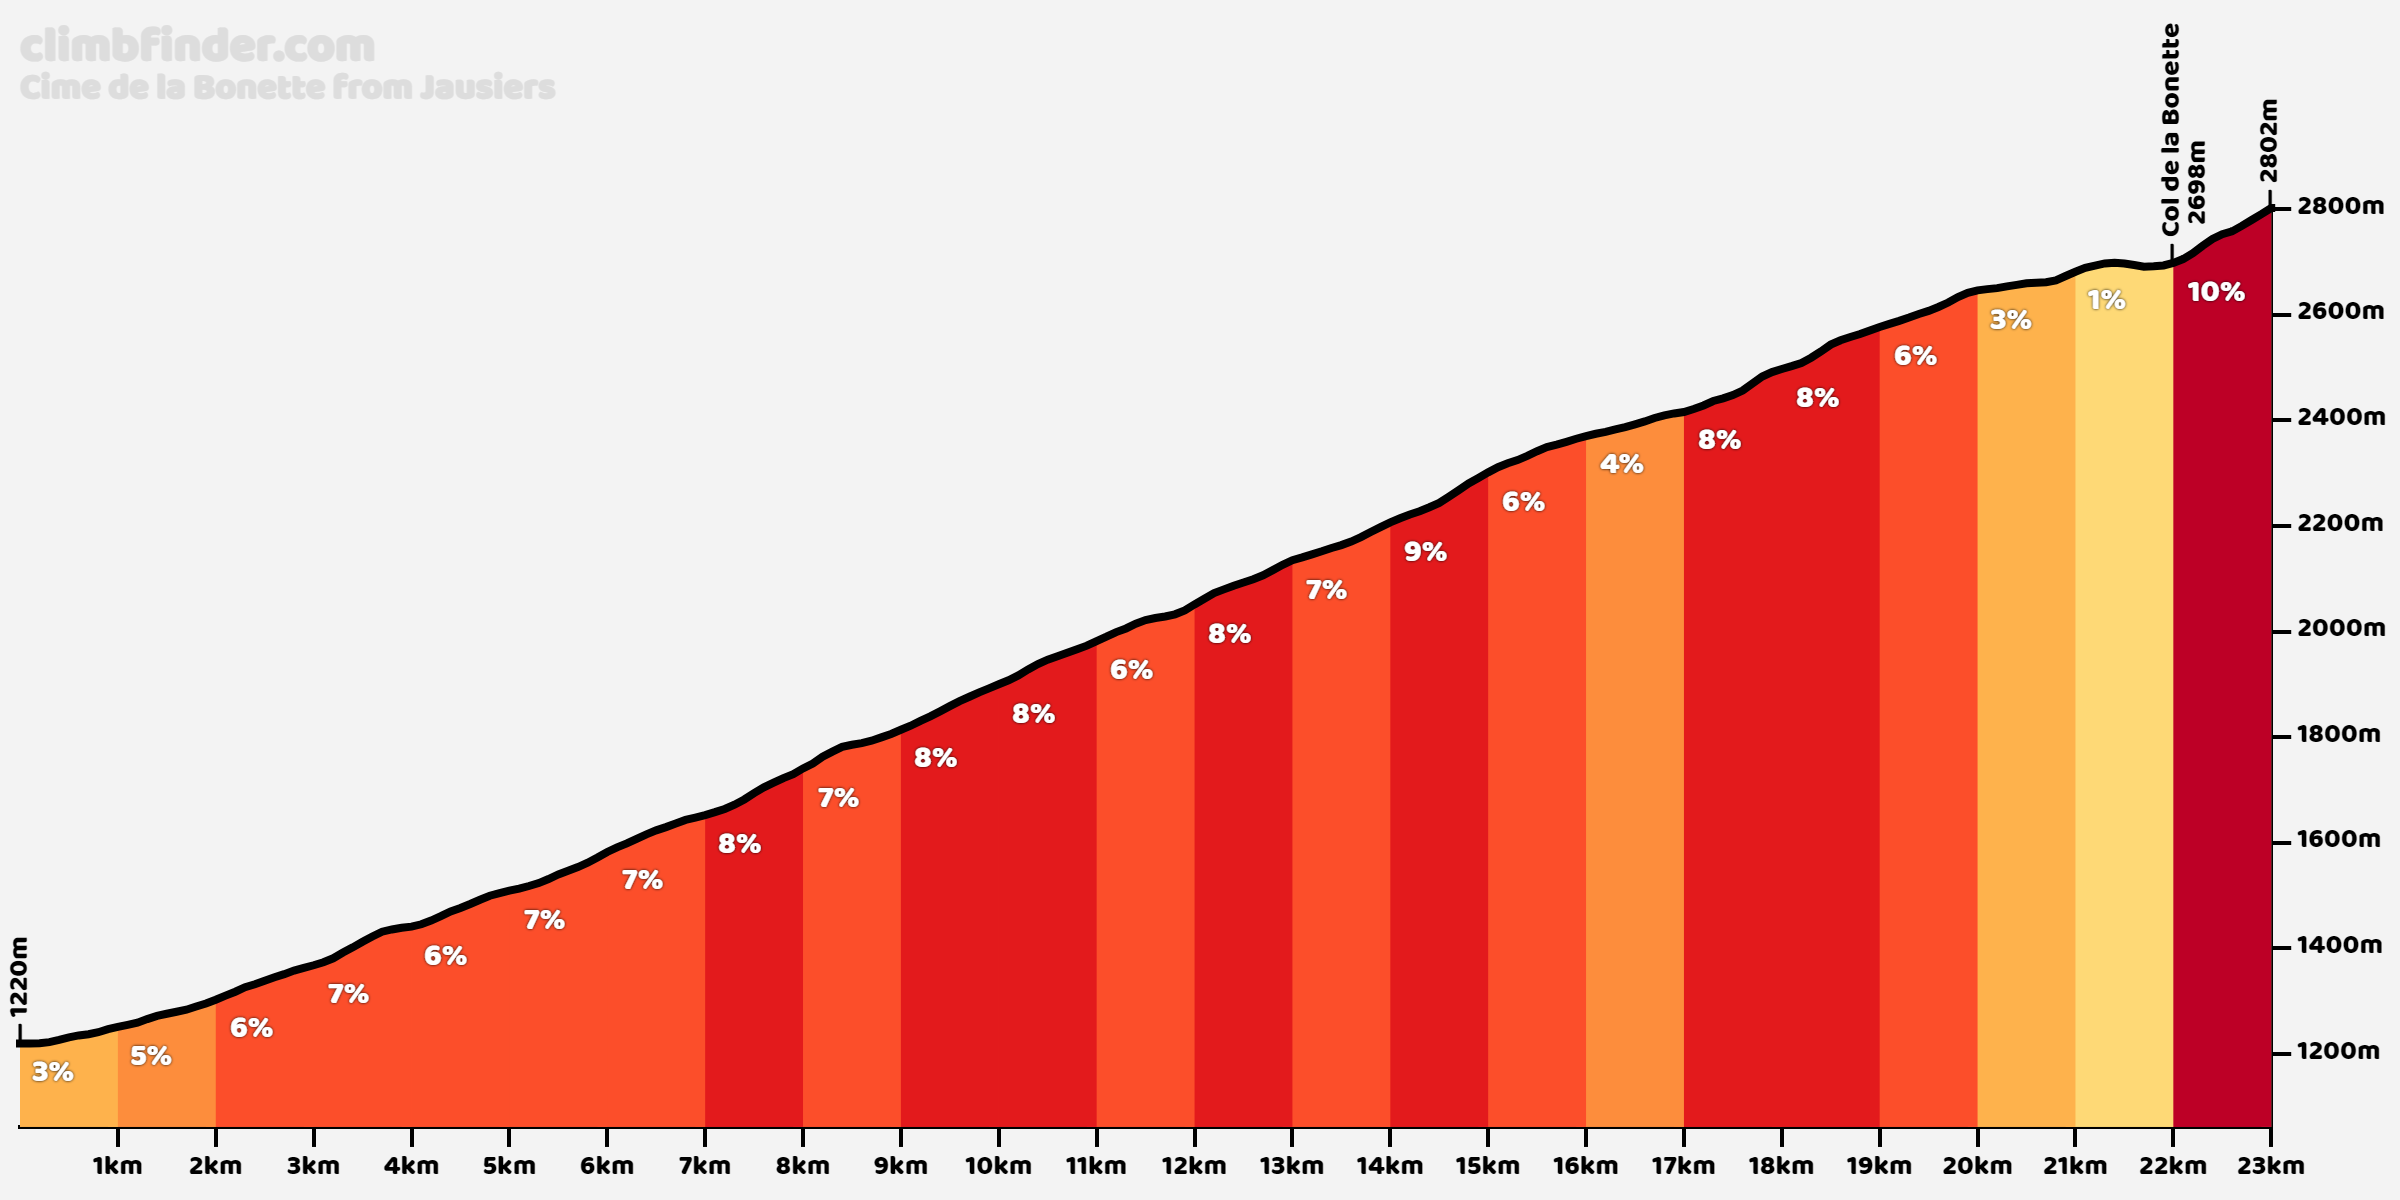
\includegraphics[width=0.72\textwidth]{obrazky/col-de-la-bonette-jausiers.png}
    \caption[]{\textbf{Zobrazení výškového profilu stoupání.} Grafické zpracování výškového profilu jediného náročného úseku stoupání v~rámci trasy pomocí sloupcového grafu.\footnotemark}
    \label{ClimbElevationProfile}
\end{figure}

\footnotetext{Převzato z: \url{https://climbfinder.com/CDN/col-de-la-bonette-jausiers.png}.}

Detailní vizuální podoba náročných částí aktivit může obsahovat údaje o~atraktivních místech, aktuální vzdálenosti, nadmořské výšce nebo sklonu stoupání, včetně barevného zvýraznění obtížnosti pro kvalitnější pochopení a~analýzu.
Zmíněná interaktivita na základě různých kritérií může přinést nový rozměr do procesu analýzy nejen celých naplánovaných cyklistických tras, ale především v~rámci náročných segmentů stoupání.
Pro tyto účely se jeví zobrazení barevnými sloupcovými grafy jako nejvíce přijatelné.

\subsection{Zobrazení frekventovaných tras v~místním okolí}
\label{display-frequent-routes-in-the-local-area}

Vizualizace frekventovaných cyklistických tras jsou ve velké míře realizovány prostřednictvím tzv. heat map\footnote{Heat mapa --~více viz \url{https://www.atlassian.com/data/charts/heatmap-complete-guide}.} neboli tepelných map.
Tato metoda využívá barevné škály k~zobrazení intenzity využití jednotlivých tras, přičemž zpravidla teplejší barvy, jako je žlutá, oranžová, nebo červená, označují oblasti s~vyšší hustotou pohybu cyklistů \cite{GuZuguang2022}.
Tento způsob znázornění umožňuje snadno identifikovat nejvyužívanější cyklostezky a~území s~výrazným pohybem, což je klíčové pro efektivní plánování aktivit nejen v~místím okolí, ale i~na celosvětové úrovni.

Jedním z~nejvíce používaných nástrojů v~této sféře je celosvětová teplotní mapa společnosti Strava\footnote{Strava Global Heatmap --~více viz \url{https://www.strava.com/maps/global-heatmap}.}, která poskytuje globální přehled o~pohybu sportovců, včetně cyklistů.
Tato služba využívá anonymizovaná data milionů uživatelů aplikace Strava k~pravidelné aktualizaci detailních map frekventovaných tras po celém světě.
Strava Global Heatmap (obrázek \ref{FrequentRoute}) umožňuje uživatelům zkoumat populární trasy a~porovnávat jejich využití v~různých geografických oblastech \cite{MarnewickMHO2018}.
Díky této funkcionalitě se jedná o~užitečný nástroj pro plánování a~analýzu cyklistických tras.

\begin{figure}[ht]
    \centering
    \includegraphics[width=0.86\textwidth]{obrazky/heatmap__5a2968df73ae9.jpg}
    \caption[]{\textbf{Zobrazení frekventovaných tras.} Mapa nejpoužívanějších cyklistických tras od výrobce sportovních navigací Strava pro evropský kontinent, vizuálně ztvárněná metodou heat map.\footnotemark}
    \label{FrequentRoute}
\end{figure}

\footnotetext{Převzato z: \url{https://images.mtbiker.sk/clanky/src/heatmap__5a2968df73ae9.jpg}.}

\section{Současná řešení analýzy a~vizualizace naplánovaných tras}
\label{current-solutions-for-analysis-and-visualisation-of-planned-routes}

Proces tvorby analýzy a~vizualizace cyklistických tras zahrnuje zevrubný průzkum husté sítě značených cest, cyklostezek a~silničních komunikací.
Jízda na kole však nemusí vždy nutně znamenat nějakou formu sportovního výkonu a~úsilí.
Zejména v~letních měsících se často jedná o~dopravní prostředek značné části populace, který slouží k~objevování a~poznávání nových zajímavých míst blízkého i~dalekého okolí.
Určení jednotlivých bodů zájmu v~rámci aktivit a~samotné naplánování přesného průběhu cyklotras je rovněž nedílnou součástí následných rozborů.

Existuje několik nástrojů a~řešení, zabývajících se uvedenou problematikou, nicméně primárním záměrem většiny jsou analýzy a~prezentace předvedených sportovních výkonů.
Detailní grafické zpracování a~podrobné vizualizace naplánovaných tras s~důrazem na náročné úseky a~pasáže stoupání však v~četné míře schází.
Některé komerční varianty jsou uživatelům dostupné v~základních a~placených prémiových verzích, ale pro účely této práce jsou podstatné především bezplatné aplikace.

\subsection{Plánovač tras Komoot}
\label{komoot-route-planner}

Komoot\footnote{Komoot Route planner -- více viz \url{https://www.komoot.com/plan}.} je platforma, která uživatelům nabízí služby primárně v~oblasti plánování pěších a~cyklistických tras.
Jedná se o~bezplatný nástroj, který je však v~několika aspektech omezen.
Více funkcí je k~dispozici registrovaným osobám, případně lze veškerý obsah využít v~rámci zpoplatněné prémiové verze.
Projekt je dostupný v~podobě webových stránek nebo jako mobilní aplikace, která je rovněž schopna zaznamenávat aktuální polohu a~stopu.
Uživatelské rozhraní ilustruje následující obrázek \ref{KomootRoutePlanner}.

\begin{figure}[ht]
    \centering
    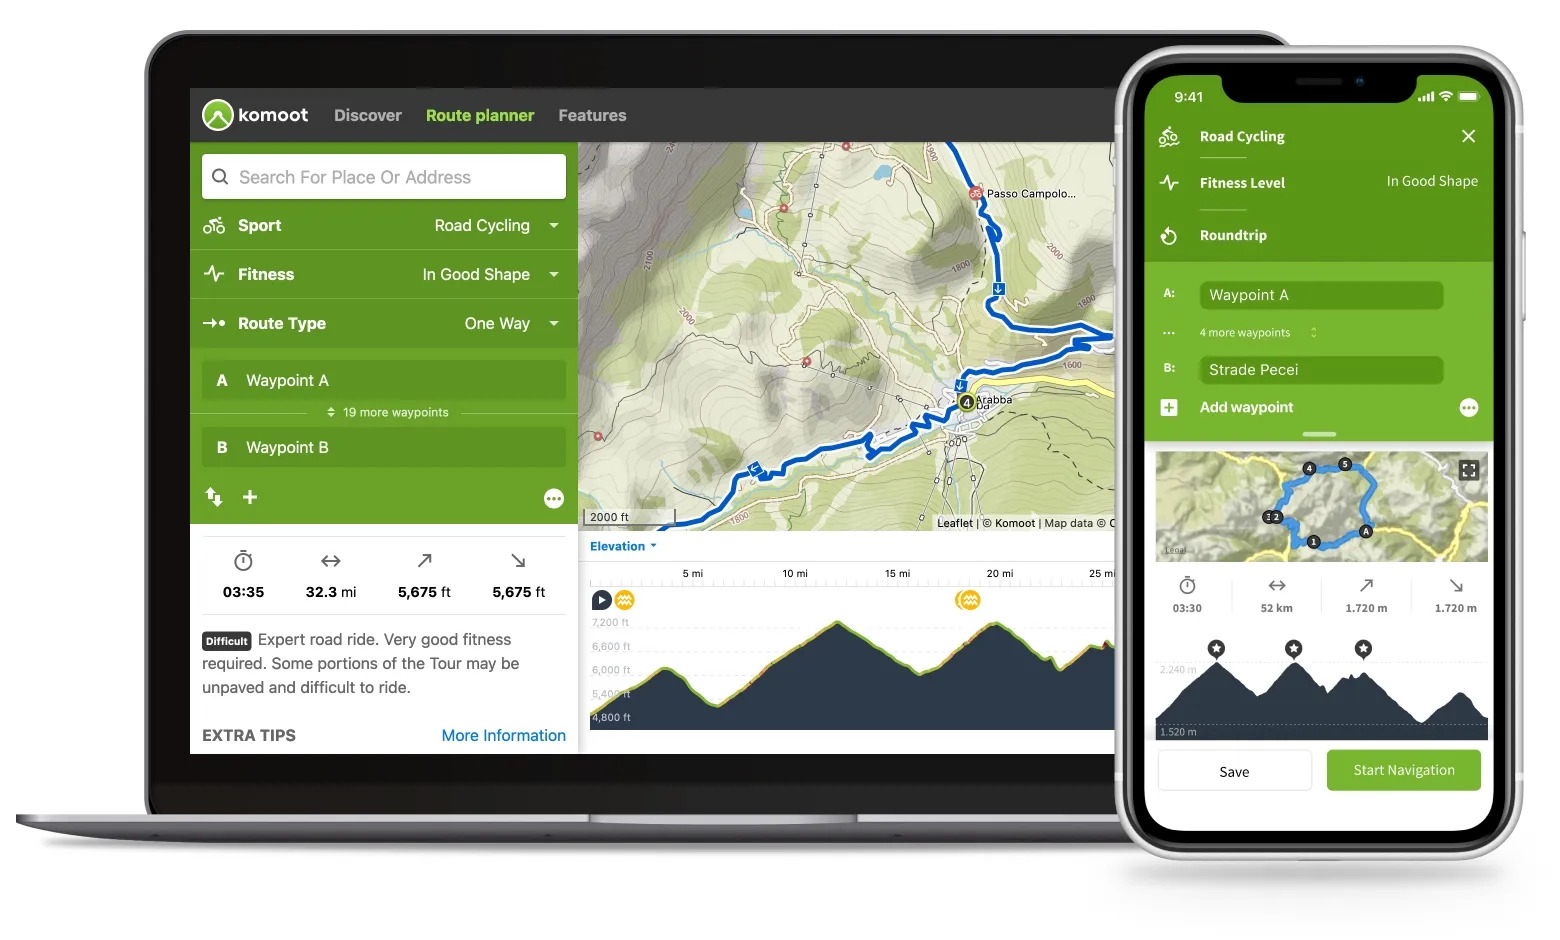
\includegraphics[width=0.86\textwidth]{obrazky/specialized-intro-v001.jpg}
    \caption[]{\textbf{Plánovač tras Komoot.} Zobrazení přesného průběhu naplánované cyklotrasy na mapovém podkladu s~doplňujícími podrobnostmi a~výškovým profilem.\footnotemark}
    \label{KomootRoutePlanner}
\end{figure}

\footnotetext{Převzato z: \url{https://www.komoot.com/images/integrations/specialized-intro-v001.jpg?q=80}.}

Plánování je možné přizpůsobit podle typu jízdního kola, přičemž na výběr jsou horská, silniční, gravel, enduro, či elektrokola.
Dílčím faktorem je momentální fyzická kondice sportovců, která má vliv na náročnost doporučených vytyčených tras.
S~tím souvisí i~přibližně stanovená obtížnost celých výletů, což představuje další pomocné vodítko.
V~neposlední řadě jsou poskytovány cenné informace o~druhu povrchu, dokreslující kompletní představu ohledně zamýšlených stop.
Využitelnou funkcionalitou je rovněž naplánování aktivit na základě předpokládaných bodů zájmu jako poznávacích okruhů, nebo jednosměrných výletů.

\subsection{Mapový portál Mapy.cz}
\label{mapy-cz-map-portal}

Snadno dostupným a~nejen mezi většinou cyklistů nejpoužívanějším mapovým portálem jsou Mapy.cz\footnote{Mapový portál Mapy.cz --~více viz \url{https://mapy.cz}.} od české společnosti Seznam.cz.
Tento projekt je veřejný a~zcela zdarma, veškeré služby jsou poskytovány prostřednictvím webu, ale pro účely orientace v~terénu a~nahrávání záznamů existuje mobilní aplikace.
Na obrázku \ref{RouteCourse} se nachází grafické uživatelské rozhraní mapového portálu během procesu plánování tras.
Podobně jako Komoot, také Mapy.cz disponují standardními výškovými profily, které obsahují základní údaje, např. nejnižší a~nejvyšší nadmořské výšky nebo celkové počty nastoupaných a~sestoupaných metrů viz obrázek \ref{RouteElevationProfile}.

Cyklisté mají možnost volby mezi horskými a~silničními koly, což pochopitelně v~určité míře ovlivňuje předběžný plán jízdy.
Při plánování jsou uživatelům, pokud možno, nabídnuty různé trasy s~odlišnou vzdáleností, převýšením a~povrchem, z~kterých je možné vybrat tu nejvhodnější.
Užitečnými funkcemi jsou počasí na trasách a~itineráře.
Ty sportovci ocení zejména v~neznámém prostředí, kde je často jedinou možností orientace podle map.
Vlastní uložené stopy lze po přihlášení k~účtu Seznam.cz jednoduše sdílet několika způsoby, a~exportovat do souborů ve formátu GPX.

\subsection{Cyklistická navigace Ride with GPS}
\label{ride-with-gps-cycling-navigation}

Ride with GPS\footnote{Ride with GPS Route Planner --~více viz \url{https://ridewithgps.com/routes/new}.} přináší alternativní řešení k~výše uvedeným nástrojům.
Platforma je přístupná přes webové stránky a~mobilní aplikaci, její základní verze je bezplatná, třebaže neobsahuje všechny možnosti a~funkce.
Obrázek \ref{RideWithGPSCyclingNavigation} prezentuje uspořádání jednotlivých prvků aplikace ve stavu plánování nových výjezdů.

\begin{figure}[ht]
    \centering
    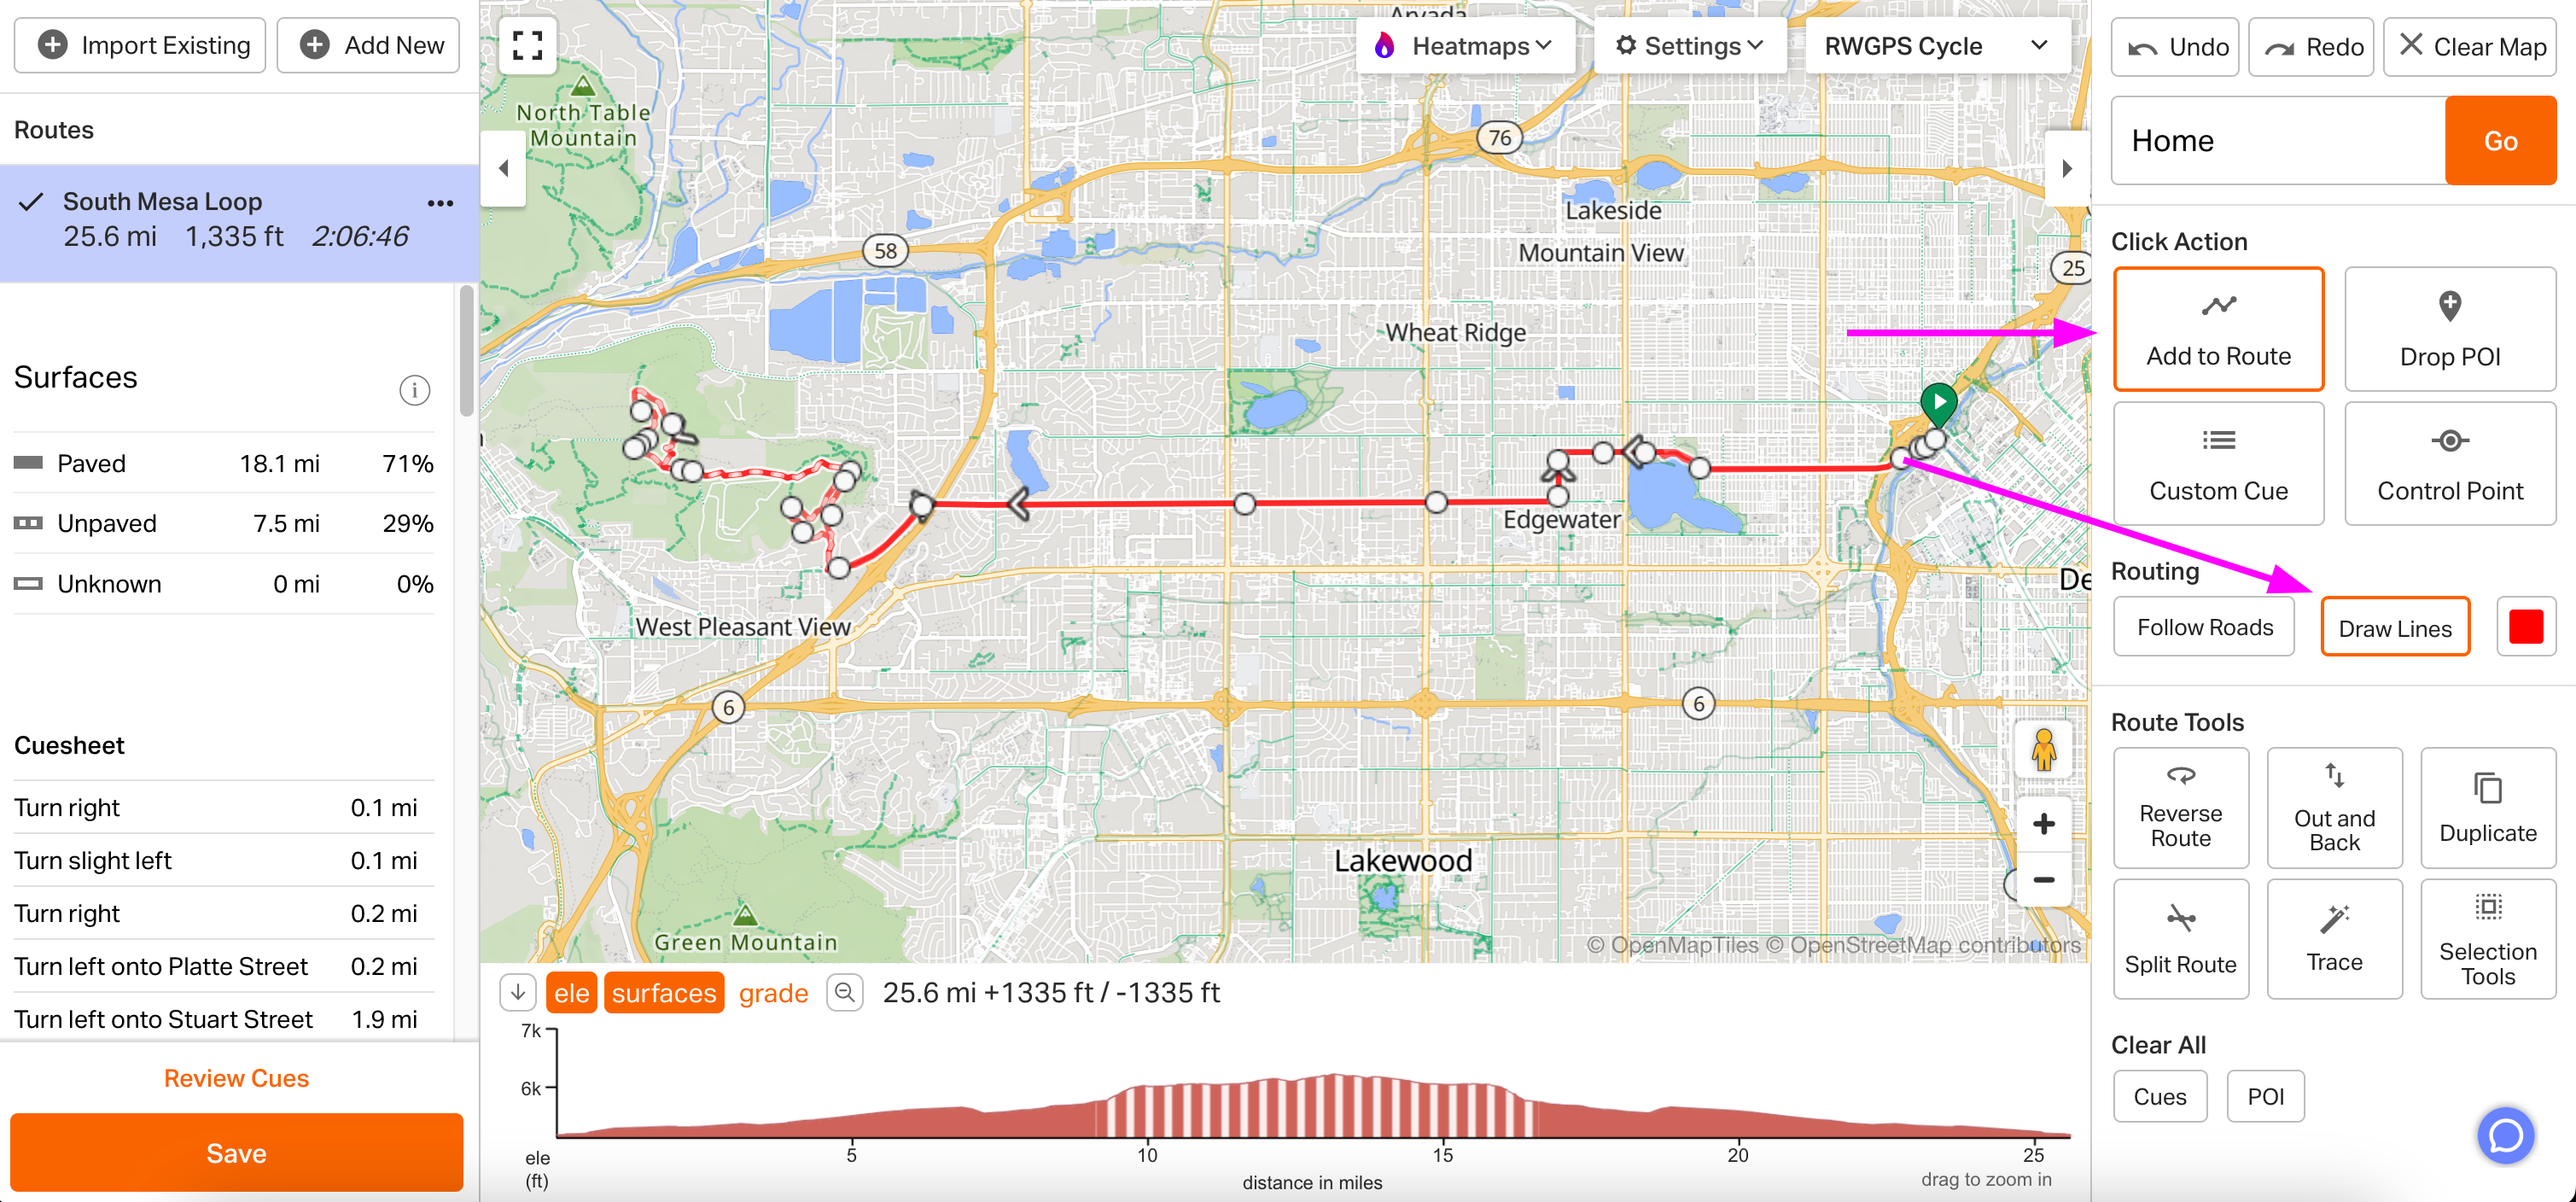
\includegraphics[width=0.86\textwidth]{obrazky/mceclip6.png}
    \caption[]{\textbf{Cyklistická navigace Ride with GPS.} Vizualizace průběhu plánované vyjížďky na mapovém podkladu s~údaji o~typu povrchu, výškovým profilem a~itinerářem.\footnotemark}
    \label{RideWithGPSCyclingNavigation}
\end{figure}

\footnotetext{Převzato z: \url{https://support.ridewithgps.com/hc/article_attachments/22912503832219}.}

Řešení umožňuje vedení zamýšlených stop po hojně využívaných komunikacích s~důrazem na cyklistickou infrastrukturu.
Uživatelé rozhodují, zda jsou upřednostňovány zpevněné, či nezpevněné cesty, současně jsou k~dispozici itineráře.
Vedle druhu povrchu je portál schopen vykreslit přibližný průběh aktuálního sklonu vozovky, avšak tato funkcionalita vede ke zkreslení výškového profilu tras.

\subsection{Internetová služba Strava}
\label{strava-internet-service}

Strava\footnote{Strava Running, Cycling \&~Hiking App --~více viz \url{https://www.strava.com}.} je celosvětově známá internetová služba, určená zejména pro sportovní nadšence v~oblasti běhu a~cyklistiky.
Aplikace slouží více méně jako sociální síť, kde uživatelé publikují své sportovní aktivity, jejichž součástí mohou být i~různé mediální soubory.
Výkony je možné nahrávat přímo prostřednictvím mobilního zařízení, nebo pomocí externích specializovaných přístrojů.
Služba však disponuje rovněž webovým rozhraním, díky kterému je prohlížení jednotlivých příspěvků dostatečně přehledné.

Platformu lze využívat zcela zdarma, avšak veškerá nabízená funkcionalita je pouze v~rámci placeného předplatného, včetně plánování vlastních tras, detailních statistik nebo osobních rekordů.
Strava se zaměřuje výhradně na analýzu již dokončených aktivit a~poskytuje vizualizace přesného průběhu stop, srdečního tepu, rychlosti, kadence šlapání, nadmořské výšky a~dokonce přibližně vypočítaného výkonu.
Uživatelské prostředí aplikace, které se neustále postupně zdokonaluje, je na obrázku \ref{StravaInternetService}.

\begin{figure}[ht]
    \centering
    \includegraphics[width=0.92\textwidth]{obrazky/Dark_Mode.png}
    \caption[]{\textbf{Internetová služba Strava.} Grafické uživatelské prostředí různých částí aplikace Strava během analýz, zaznamenávání tras a~procházení osobních statistik.\footnotemark}
    \label{StravaInternetService}
\end{figure}

\footnotetext{Převzato z: \url{https://images.ctfassets.net/9olkiac82a1q/25RSlcP0rph2RwBa5PWF5W/1a0bfa4b5d38b4a89c3f635a9848191e/Dark_Mode.png}.}

\subsection{Webový server Climbfinder}
\label{climbfinder-web-server}

Server Climbfinder\footnote{Climbfinder --~více viz \url{https://climbfinder.com/en}.} se specializuje výlučně na cyklisty, nabízí podrobné informace a~výškové profily vybraných stoupání a~náročných úseků na evropském kontinentu viz obrázek \ref{ClimbElevationProfile}.
Grafické vizualizace nejsou interaktivní a~služba neumožňuje tvorbu vlastních náročných segmentů.
Navíc je plánování tras k~dispozici pouze v~prémiové verzi.

\section{Shrnutí současného stavu}
\label{summary-of-the-current-situation}

Momentálně je k~dispozici celá řada dostupných geografických dat a~různých metod vizuálního zprostředkování naplánovaných tras.
Pro analýzu jednotlivých tras jsou nezbytné zdroje geografických dat, které lze rozdělit na dvě hlavní skupiny.
Primární zdroje zahrnují data získaná vlastním měřením pomocí GPS zařízení.
Naopak sekundární zdroje představují existující otevřené mapové sady a~aplikace, které umožňují snadné plánování aktivit a~jejich případný export ve vhodných formátech.

Důležité jsou rovněž způsoby transformace surových geografických dat na srozumitelnější grafické výstupy.
Mezi klíčové metody patří zobrazení průběhu tras na mapě, vizualizace výškových profilů či identifikace náročných úseků.
Tyto reprezentace napomáhají sportovcům lépe pochopit obtížnost tras, připravit se na kritická místa a~efektivněji plánovat své výkony.

V~neposlední řadě mohou uživatelé využívat současné nástroje pro analýzu a~vizualizaci nejen cyklistických tras.
Představené platformy nabízejí široké spektrum funkcí, od detailního plánování tras, výpočtu převýšení a~dalších vybraných statistik až po přehled oblíbených bodů zájmu nebo specifických zajímavostí.
Přestože jsou základní verze většiny těchto aplikací zdarma, některé prémiové funkce vyžadují předplatné.

Celkově se ukazuje, že detailní analýzy a~grafické vizualizace sportovních aktivit tvoří spojení geografických dat, moderních technologií a~uživatelsky přívětivých aplikací.
Tyto aspekty přispívají k~efektivnímu plánování a~vylepšení zážitku z~cyklistiky, ať už jde o~rekreační, sportovní, nebo dopravní využití jízdních kol.

\chapter{Plánování sportovních aktivit podle náročnosti vytyčených cílů}
\label{planning-of-sports-activities-according-to-the-difficulty-of-the-marked-goals}

Moderní technologie umožňují sportovcům analyzovat klíčové parametry tras a~díky tomu přizpůsobit intenzitu a~objem tréninků individuálním potřebám a~schopnostem.
Data získaná z~globálních satelitních navigačních systémů, topografické mapy, klimatické podmínky a~další relevantní informace pomáhají sportovcům adekvátně se připravit na konkrétní výzvy spojené s~trasami a~optimalizovat svoje výkony podle náročnosti terénu.

Správně nastavené tréninkové plány, odpovídající specifikům jednotlivých aktivit, a~jejich využití napomáhá aktivním jedincům zvolit optimální rychlost a~tempo, šetřit energii či předejít přetížení organismu.
S~těmito možnostmi se plánování sportovních výkonů stává procesem, který přináší vyšší efektivitu tréninků, podporuje dlouhodobý růst výkonnosti a~může sloužit k~prevenci zranění.

Plánování sportovních výkonů v~kontextu cyklistiky hraje zásadní roli pro efektivní dosažení osobních cílů a~bezpečné dokončení vytyčených tras.
Vzhledem k~různorodosti cyklistických výjezdů je potřeba zohlednit nejen vzdálenosti, ale i~další nezanedbatelné faktory, kterými jsou celkové převýšení, obtížnost vybraných úseků a~pasáží nebo náročnost naplánovaných cyklotras.
Tyto aspekty mohou výrazně ovlivnit požadovaný výkon a~energetický výdej cyklistů.

\section{Plánování sportovních výkonů}
\label{sport-performance-planning}

Během posledních let se plánování a~analýzy sportovních činností neustále zdokonalují značným tempem.
Nejde pouze o~materiální vybavení, ale objevují se i~nové tréninkové metody a~nástroje zvyšující efektivitu vynaloženého úsilí.
Momentálně mají sportovci možnost využívat všemožná trasovací zařízení, snímače rychlosti pohybu, kadence a~v~poslední době se rozšiřují také měřiče výkonu s~tím, jak klesá jejich pořizovací cena \cite{HopkerJames2012}.

V~současné době se do plánování sportovních aktivit zapojuje široká škála digitálních nástrojů a~aplikací, které usnadňují tvorbu těchto tréninkových plánů.
Tato řešení přináší sportovcům a~trenérům nové možnosti přístupu k~plánování strukturovaným způsobem.

Vlastní proces plánování se významně liší v~závislosti na tom, zda jsou studovanými aktivitami individuální sporty, ligové soutěže, případně týmové sporty.
Zatímco pro ligové soutěže je vhodný systematický přístup, který se dokáže adaptovat na předešlé výkony a~výsledky, týmový sport je otázkou komplexního procesu, který představuje další výzvy \cite{LyleJohn2010}.
Sportovní odvětví, v~nichž hrají zásadní roli jednotlivci, vyžadují plánování zaměřené na optimalizaci individuálních výkonů a~přizpůsobení tréninkových metod konkrétním potřebám sportovců.

Ačkoliv základní struktura zůstává pro většinu individuálních sportů podobná, jednotlivé kategorie se liší svými specifickými požadavky, jako je technická příprava, intenzita zátěže nebo zaměření na psychologickou stránku.
Tento rozdíl reflektuje jedinečné nároky každé sportovní oblasti, které ovlivňují detaily celého plánovacího procesu.
Existují jednak univerzální tréninkové plány v~rámci aplikací pro všeobecnou fyzickou aktivitu, ale také specializované postupy určené přímo na míru jednotlivým sportům.
Ve většině případů ani nezáleží na tom, zda jsou daní uživatelé profesionálové, nebo se jedná o~začínající sportovce, případně amatéry.

Mezi nejoblíbenější sportovní aplikace patří Strava, blíže popsána v~sekci \ref{strava-internet-service}, kterou využívají především běžci a~cyklisté a~nyní se již jedná v~podstatě o~sociální síť pro sportovce, jelikož podporuje sdílení více než 30 druhů sportovních výkonů.
Dalšími hojně využívanými službami jsou například MyFitnessPal\footnote{MyFitnessPal --~více viz \url{https://www.myfitnesspal.com}.}, Nike Run Club\footnote{Nike Run Club --~více viz \url{https://www.nike.com/nrc-app}.}, Garmin Connect\footnote{Garmin Connect --~více viz \url{https://connect.garmin.com}.} a~mnoho dalších.
Součástí těchto řešení je nejen možnost stanovení osobních cílů, zapojení se do týdenních, či měsíčních výzev, ale pro soutěživé jedince rovněž příležitost porovnání se s~přáteli a~ostatními sportovci.

Plánování sportovních výkonů je každopádně jedinečným procesem, který si ponechává základní principy.
Ať už se týká jakéhokoliv sportu, je založeno na důkladných rozborech aktuální fyzické kondice, technické a~taktické vyzrálosti jedinců, využívá současných vědeckých znalostí v~daných oblastech, adekvátně se dokáže přizpůsobit na základě nových zjištění a~zpětné vazby a~jeho logické uspořádání odpovídá stanoveným ambicím \cite{ManilalKPDr2021}.
Tento proces zahrnuje nejen analýzu fyzických a~technických parametrů, ale také hluboké porozumění specifických podmínek, které mohou ovlivnit výkony, a~to jak na úrovni jednotlivců, tak v~kontextu celých sportovních aktivit.

\section{Objektivní a~subjektivní faktory náročnosti aktivit}
\label{objective-and-subjective-factors-of-activity-difficulty}

Pohledy na obtížnost naplánovaných tras jsou ve většině případů různé, dalo by se konstatovat až subjektivní, analogicky to platí rovněž pro určité náročnější segmenty a~úseky stoupání.
Jedním možným způsobem, kterým lze rozdělit jednotlivé faktory ovlivňující náročnost sportovních aktivit, je právě na základě jejich lidského vnímání.
Uvedené okolnosti tedy mohou být vnímány buď objektivně, nebo subjektivně.

Co se týče subjektivních faktorů, do této kategorie lze zařadit proměnné, které mají v~rozdílných situacích odlišný vliv na obtížnost.
Mezi tyto činitele se bezpochyby řadí hmotnost sportovců a~jízdních kol, valivý odpor různých druhů používaných cyklistických plášťů, odpor vzduchu, konkrétní kombinace převodů a~jejich adekvátně nastavené poměry \cite{SwainDavidP1998}, dále fyzická kondice, pohybové schopnosti, technika a~taktika, ale také psychika či somatické faktory.
Tyto údaje se však liší nejen pro různé typy jízdních kol a~komponentů, ale rovněž pro téměř každého sportovce.

Pro účely této práce jsou daleko relevantnější a~významnější faktory objektivní, které mají pro identické trasy stejný vliv na obtížnost za jakýchkoliv okolností.
Za obecná kritéria klasifikace obtížnosti celých naplánovaných cyklistických výletů se obvykle považuje celková vzdálenost a~převýšení, počet nastoupaných metrů či typ terénu.
Dalšími objektivními faktory, které mohou zásadním způsobem ovlivnit výkony, jsou průměrná a~maximální nadmořská výška.
Pro náročné pasáže stoupání jsou důležitými ukazateli nejen dílčí vzdálenost, ale také průměrný a~maximální sklon, průběh a~pravidelnost kopců, počet nastoupaných metrů nebo cílová nadmořská výška vrcholů.
Na základě všech těchto věcných měřítek je možné alespoň do jisté míry nezávisle určit obtížnost sportovních aktivit a~úseků stoupání.

Největším cyklistickým etapovým závodem na světě je zcela jistě Tour de France\footnote{Tour de France --~více viz \url{https://www.letour.fr/en/}.}.
Trasa každoročně obsahuje ikonická stoupání na vrcholy ve vysokých nadmořských výškách.
Pro ilustraci, zdroj \cite{WarrenSimon2014} popisuje 100 vybraných kopců v~rámci tohoto slavného závodu a~přináší jejich hodnocení v~kontextu publikace.
Následně však není možné nezaujatým způsobem porovnávat náročnost stoupání, která nejsou uvedena v~daném výčtu.
Hlavní pozornost je tedy nadále věnována převážně objektivním faktorům náročnosti.

\section{Postupy výpočtu objektivních faktorů náročnosti aktivit}
\label{procedures-for-calculating-objective-activity-difficulty-factors}

Úroveň obtížnosti celých naplánovaných tras může sportovcům sloužit jako indikátor, zda jsou schopni požadované etapy zvládnout, nebo zda se jedná již o~příliš náročné výzvy.
Obtížnost jako taková se skládá z~objektivních parametrů, jako jsou celková vzdálenost tras, převýšení či počet nastoupaných metrů.
Zároveň ji však ovlivňují i~subjektivní faktory, například fyzická kondice a~mentální připravenost jedinců.

Celková vzdálenost výjezdů je jedním z~nejviditelnějších parametrů, který má vliv na výslednou obtížnost.
Ve spojení s~převýšením poskytuje základní údaj o~potenciálním energetickém výdeji a~době trvání sportovních aktivit.
Náročnost vytyčených tras je ovlivněna mimo jiné jejich povrchem, přičemž rozdíl je patrný mezi komunikacemi vedoucími výhradně po asfaltových či jinak zpevněných cestách a~těmi, které kopírují horské traily a~singletracky\footnote{Singletrack --~více viz \url{https://en.wikipedia.org/wiki/Single_track_(mountain_biking)}.}.
Terén má vliv na rychlost pohybu, nároky na rovnováhu i~svalovou koordinaci.
Trasy ve vyšších nadmořských výškách kladou mnohem větší nároky na dýchací soustavu kvůli nižší koncentraci kyslíku ve vzduchu.
To se projevuje zejména při dlouhých stoupáních ve vysokohorských oblastech.

Pro hodnocení obtížnosti sportovních výkonů existuje několik metod, přičemž žádná z~nich není univerzální.
Tyto metody obvykle kombinují výše uvedené faktory do jednoho celkového skóre.
Numerická hodnocení jsou poměrně složitě interpretovatelná, jelikož vyžadují určitý kontext ve smyslu škálovatelného měřítka.
Pro jednotlivce má však stanovení obtížnosti praktický význam především z~hlediska přípravy, správného plánování a~minimalizace rizik.
Kromě toho je důležité zohlednit individuální schopnosti sportovců, které mohou mít zásadní vliv na to, jestli jsou schopni se na vybrané trasy vhodně adaptovat a~přizpůsobit jim svou výbavu a~fyzickou přípravu.

Samostatným fenoménem jsou úseky stoupání, představující specifické části tras, které podstatným způsobem ovlivňují komplexní náročnost sportovních výkonů.
Zatímco celková obtížnost tras poskytuje obecný přehled, detailní analýza konkrétních stoupání a~vybraných segmentů umožňuje podrobněji zhodnotit výzvy, které aktivita zahrnuje.
Grafická vizualizace těchto částí se zobrazením důležitých statistik a~aspektů každé náročné pasáže nachází využití zejména při důkladném plánování výkonů.

Pro zmiňované části tras jsou klíčovými měřítky nejen dílčí vzdálenost, průměrný a~maximální sklon, ale také jejich průběh v~celé délce, zda jsou stoupání konstatní, či se jejich sklon výrazně mění, dále konečná nadmořská výška, celková suma nastoupaných metrů a~v~neposlední řadě umístění nejstrmějších úseků.
Tyto a~další podobné údaje jsou v~surové formě čísel, tudíž jejich podrobné grafické znázornění formou vizualizace zprostředkuje nezbytné informace efektivní a~účinnou cestou.

Obdobně jako pro celé naplánované trasy, rovněž v~případě hodnocení náročnosti určitých úseků stoupání existuje několik variant objektivního posouzení.
Pro zachování jednoduchosti a~kontinuity je jednou z~možností ohodnocení těchto segmentů varianta s~využitím číselných indexů obtížnosti.
Tento způsob umožňuje nezávisle porovnávat náročnost pasáží z~různých koutů světa na základě stejného ukazatele.

Vstupní data, obsahující naplánované trasy s~veškerými potřebnými detaily, mohou být součástí souborů odlišných formátů od FIT, GPX, KML až po TCX, rozebranými v~sekci \ref{methods-of-obtaining-and-storing-geographic-data}.
Tyto zdrojové soubory zahrnují seznamy bodů se zeměpisnými souřadnicemi a~nadmořskými výškami.
Jelikož se tato práce zabývá primárně objektivním hodnocením úrovně obtížnosti, podstatnými kritérii jsou především celková vzdálenost, počet nastoupaných a~sestoupaných metrů a~průměrný a~maximální sklon v~rámci sportovních aktivit.

\subsection{Výpočet celkové vzdálenosti aktivit a~úseků stoupání}
\label{calculation-of-total-activity-distances-and-climb-sections}

Vzdálenost naplánovaných sportovních aktivit lze vypočítat na základě sekvence GPS bodů, která definuje jejich průběh.
Každý GPS bod obsahuje zeměpisnou šířku a~délku a~případně i~nadmořskou výšku.
V~geografických systémech a~aplikacích se k~výpočtu vzdálenosti mezi dvěma po sobě jdoucími body nejčastěji využívá Haversinův vzorec \cite{IchramsyahMochamadK2024}, jehož diagram je na obrázku \ref{HaversineFormula}.

Matematicky lze vzdálenost $l$~mezi dvěma body $P$~a~$Q$, definovanými souřadnicemi $(\phi_P, \lambda_P)$ a~$(\phi_Q, \lambda_Q)$, vyjádřit jako:

\[
    l = 2r \times \arcsin \left( \sqrt{\sin^2\left(\frac{\phi_Q - \phi_P}{2}\right) + \cos(\phi_P) \times \cos(\phi_Q) \times \sin^2\left(\frac{\lambda_Q - \lambda_P}{2}\right)} \right)
\]

kde:
\begin{itemize}
    \item $r$~je poloměr Země, přičemž v~průměru dosahuje přibližně 6\,371\,km\footnote{Earth Fact Sheet -- více viz \url{https://nssdc.gsfc.nasa.gov/planetary/factsheet/earthfact.html}.},
    \item $\phi$~je zeměpisná šířka v~radiánech,
    \item $\lambda$~je zeměpisná délka v~radiánech.
\end{itemize}

\begin{figure}[ht]
    \centering
    \includegraphics[width=0.36\textwidth]{obrazky/Illustration_of_great-circle_distance.svg.png}
    \caption[]{\textbf{Haversinův vzorec.} Diagram znázorňující velkokružnicovou vzdálenost mezi dvěma body na kouli $P$~a~$Q$, zobrazeny jsou také dva antipodální body $u$~a~$v$.\footnotemark}
    \label{HaversineFormula}
\end{figure}

\footnotetext{Převzato z: \url{https://upload.wikimedia.org/wikipedia/commons/thumb/c/cb/Illustration_of_great-circle_distance.svg/440px-Illustration_of_great-circle_distance.svg.png}.}

Výsledná vzdálenost trasy $L$~se vypočítá jako součet dílčích vzdáleností mezi všemi po sobě jdoucími GPS body, kde $n$~je počet bodů, ze kterých se trasa skládá:

\[
    L = \sum_{i=1}^{n-1} l_i
\]

Vzdálenost vybraných úseků stoupání je možné stanovit stejnou metodou jako celkovou vzdálenost naplánovaných tras.
Každá část stoupání je definována posloupností GPS bodů s~postupně rostoucími nadmořskými výškami, přičemž kratší klesající pasáže jsou považovány za jejich nedílné součásti.
V~takových případech se vzdálenost započítává kontinuálně bez přerušení.

Existuje mnoho dalších způsobů, kterými je možné vyjádřit vzdálenost mezi dvěma GPS body, ale pro účely této práce je Haversinův vzorec dostačující.
Metoda je pro kratší vzdálenosti poměrně spolehlivá, zatímco si ponechává svou jednoduchost.
Vzhledem k~tomu, že pracuje pouze se zeměpisnými šířkami a~délkami, je vhodná pro výpočty v~případech, kdy nejsou rozdíly v~nadmořských výškách klíčové.
Díky své snadné implementaci a~dostatečné přesnosti poskytuje efektivní řešení pro většinu praktických účelů.

\subsection{Výpočet celkového počtu nastoupaných a~sestoupaných metrů}
\label{calculation-of-the-total-number-of-meters-ascended-and-descended}

Celkový počet nastoupaných a~sestoupaných metrů se řadí mezi další objektivní faktory, které mají významný podíl na obtížnosti naplánovaných tras.
Tyto údaje je možné získat prostřednictvím jednotlivých GPS bodů, které vedle samotných zeměpisných souřadnic obsahují zpravidla i~nadmořské výšky.
Alternativou je stanovení nadmořských výšek ze zeměpisných šířek a~délek s~využitím vhodného digitálního modelu terénu\footnote{Digital elevation model (DEM) -- více viz \url{https://www.usgs.gov/faqs/what-a-digital-elevation-model-dem}.}, pokud nejsou tato data obsažena explicitně.

Díky tomu, že se při plánování tras pohybují vzdálenosti mezi GPS body v~jednotkách, maximálně desítkách metrů, není nezbytně nutné zohledňovat skutečný tvar zemského povrchu.
Je tedy možné výpočty zjednodušit a~jako celkový počet nastoupaných a~sestoupaných metrů označit součet přírůstků, potažmo úbytků, hodnot nadmořských výšek každých dvou po sobě jdoucích GPS záznamů.

Pro stanovení celkového počtu nastoupaných ($A$) a~sestoupaných ($B$) metrů mezi GPS body je možné postupovat tak, že pokud každý bod trasy $P_i$ obsahuje informaci o~nadmořské výšce $a_i$ a~kompletní aktivita je tvořena sekvencí $n$~bodů $P_1, P_2, \dots, P_n$, poté rozdíl nadmořských výšek $\Delta a_i$ mezi dvěma sousedními body $P_i$ a~$P_{i+1}$ lze vyjádřit jako:

\[
    \Delta a_i = a_{i+1} - a_i
\]

Rozdíly nadmořských výšek $\Delta a_i$ jsou následně rozčleněny na dvě skupiny.
Kladné změny nadmořských výšek reprezentují přírůstky ($\Delta a_i > 0$) a~záporné změny naopak úbytky ($\Delta a_i < 0$).
Celkový počet nastoupaných metrů $A$~(\ref{MetersAscended}) a~sestoupaných metrů $B$~(\ref{MetersDescended}) lze vypočítat takto:

\begin{align}
    A =& \sum_{\Delta a_i > 0} \Delta a_i \label{MetersAscended} \\
    B =& \sum_{\Delta a_i < 0} |\Delta a_i| \label{MetersDescended}
\end{align}

Tento typ výpočtu předpokládá, že nadmořské výšky jsou pro veškeré GPS body přesné.
V~praxi se však poměrně často vyskytují chyby způsobené omezenou přesností lokalizačních systémů.
Pro minimalizaci šumu je možné aplikovat filtrační metody, například klouzavý průměr \cite{OzdemirZeynep2019}.
Při výpočtech na úrovni metrů může šum v~nadmořských výškách způsobit nadhodnocení či podhodnocení nastoupaných a~sestoupaných metrů.
Z~tohoto důvodu je vhodné ignorovat změny menší než adekvátně zvolený práh.

Celkový počet nastoupaných a~sestoupaných metrů představuje klíčový parametr pro hodnocení obtížnosti naplánovaných tras.
Přesnost tohoto výpočtu je závislá nejen na kvalitě samotných dat, ale také na způsobu zpracování a~případné aplikaci filtrů.
Výsledné hodnoty nacházejí využití při analýze tras, plánování sportovních výkonů nebo hodnocení fyzické náročnosti.

Stejný princip platí i~pro výpočty dílčích množství nastoupaných a~sestoupaných metrů v~rámci segmentů stoupání.
Ve většině případů jsou sestoupané metry irelevantní, ale pokud jsou tato čísla nezanedbatelná, mají obecně jistý vliv na náročnost stoupání.
Rovnice \ref{MetersAscended} a~\ref{MetersDescended} vyjadřují přesné postupy, kterými se lze dopracovat k~očekávaným hodnotám.

\subsection{Výpočet dílčího průměrného a~maximálního sklonu stoupání}
\label{calculation-of-partial-average-and-maximum-slopes}

Podstatnou metrikou při evaluaci náročných výzev je průměrný a~maximální sklon stoupání.
Maximální sklon je určen jako nejstrmější úsek v~rámci této části trasy.
Vypočítá se jako poměr rozdílu nadmořských výšek a~horizontální vzdálenosti mezi dvěma po sobě jdoucími GPS body, přičemž jejich přesnost závisí na kvalitě a~četnosti GPS záznamů.
Kvůli popsaným omezením je patřičnou alternativou k~absolutním maximálním sklonům identifikace nejstrmějších úseků stoupání v~rozumné délce, např. 100\,m, 200\,m, 500\,m~či 1\,000\,m.
Tyto vzdálenosti závisí na celkové délce vybraných stoupání.

\begin{figure}[ht]
    \centering
    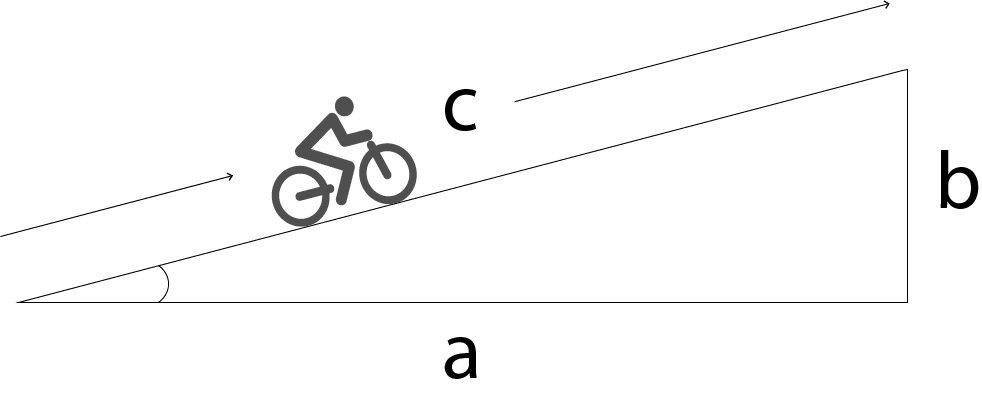
\includegraphics[width=0.64\textwidth]{obrazky/gradient.png}
    \caption[]{\textbf{Výpočet průměrného sklonu.} Průměrný sklon ($c$) je daný poměrem rozdílu nadmořských výšek ($b$) a~horizontální vzdálenosti ($a$).\footnotemark}
    \label{ClimbGradient}
\end{figure}

\footnotetext{Převzato z: \url{https://cyclingmagazine.ca/wp-content/uploads/2020/05/gradient.png}.}

Naopak průměrný sklon stoupání je možné určit pomocí jednoduchého vzorce na základě obrázku \ref{ClimbGradient}.
Liší se však to, jestli jsou do stoupání zahrnuty rovinaté a~klesající úseky.
Průměrný sklon čistě stoupajících částí věrně popisuje náročnost, zatímco celkový průměrný sklon i~s~těmito jednoduššími pasážemi může sloužit jako vodítko, zda se ve stoupání vyskytují nějaké snazší úseky, či dokonce sjezdy.
Vzorec, sloužící k~výpočtu průměrného sklonu $c$~v~procentech, je následující:

\[
    c = \frac{b}{a} \times 100\,\%
\]

kde:
\begin{itemize}
    \item $b$~je rozdíl nadmořských výšek mezi dvěma GPS body v~metrech,
    \item $a$~je vzdálenost mezi dvěma GPS body v~metrech.
\end{itemize}

\subsection{Identifikace úseků stoupání v~rámci naplánovaných aktivit}
\label{identification-of-climb-sections-within-planned-activities}

Podstatnou částí je samotné rozpoznání jednotlivých segmentů stoupání a~jejich následné korektní zpracování.
K~tomuto účelu je nutná důsledná analýza GPS záznamů s~odpovídajícími nadmořskými výškami.
Pasáže naplánovaných tréninků jsou označeny jako stoupání, pokud vykazují celkový nárůst nadmořských výšek.
Krátké roviny a~klesání jsou do stoupání rovněž zahrnuty, aby odpovídaly reálným terénním podmínkám.

Sekvence GPS bodů, které se jeví jako potenciálně obtížné, se ovšem nemusí za každou cenu řadit mezi náročné úseky, protože se jedná například o~velmi krátké a~okamžité změny sklonu.
Není tedy vždy žádoucí pojímat veškeré takové části jako náročná stoupání.
K~těmto účelům slouží objektivní ohodnocení a~pokud je vyšší než stanovená hranice, je možné takové segmenty považovat za stoupání.

\section{Definice koeficientů ovlivňujících fyzickou náročnost}
\label{definitions-of-coefficients-affecting-physical-demand}

Pro objektivní určení číselného ohodnocení náročnosti celých naplánovaných tras a~dílčích stoupání je nezbytné zohlednit více parametrů, které mají vliv na fyzickou obtížnost překonávaných terénů.
Kromě zřejmých faktorů, jakými jsou vzdálenost a~průměrný sklon, hrají neméně významnou roli také typ povrchu nebo počáteční a~koncová nadmořská výška s~ohledem na proměnlivé koncentrace kyslíku ve vzduchu\footnote{Závislost mezi nadmořskou výškou a~obsahem kyslíku ve vzduchu --~více viz \url{http://www.praha.cz/karel/kyslik.html}.}.

Matematicky lze základní index náročnosti dílčího úseku trasy ($d_i$) vyjádřit jako podíl druhé mocniny průměrného sklonu ($s_i^2$) v~procentech a~jeho vzdálenosti ($l_i$) v~metrech, jak uvádí publikace \cite{GodeLegrosJP1990}:

\[
    d_i = \frac{s_i^2}{l_i}
\]

Pokud se průměrný sklon dílčího úseku trasy pohybuje v~neutrálních či záporných hodnotách, je nutné tuto část považovat za obtížnější, jelikož i~rovinaté a~klesající pasáže vyžadují určitý výdej energie a~v~případě nepřihlédnutí k~tomuto faktu je index náročnosti daleko menší.
Jedním z~možných řešení je pro takové segmenty určit referenční průměrný sklon na hodnotu~1\,\%.
Tímto způsobem je do jisté míry zachována odpovídající obtížnost méně kopcovitých naplánovaných tras a~stoupání.

Analyzované segmenty mají počáteční a~koncovou nadmořskou výšku, ze kterých lze určit průměrnou nadmořskou výšku.
Čím vyšší je tato hodnota, tím fyzicky náročnější je jeho zdolání díky výše zmíněným měnícím se podmínkám.
Zároveň se střídají typy povrchu, které mohou být asfaltové, betonové, zpevněné, šotolinové, nezpevněné, kamenité aj.
To do jisté míry rozhoduje o~tom, jak efektivně se přeměňuje vyprodukovaná energie do rychlosti pohybu.
Proto je podle článku \cite{JewettMatthew2024} vhodné přidat odpovídající koeficient, který reflektuje tento faktor.

\subsection{Koeficient vlivu průměrné nadmořské výšky}
\label{effect-coefficients-of-average-altitudes}

Pro různé hodnoty průměrné nadmořské výšky částí naplánovaných tras a~úseků stoupání je stanoven koeficient ($f_a$), který je zjednodušeně přímo závislý výhradně na nadmořské výšce.
Ačkoliv ve skutečnosti je ovlivněn např. relativní vlhkostí vzduchu, atmosférickým a~relativním tlakem, sycením krve kyslíkem, relativním množstvím kyslíku, hustotou vzduchu nebo teplotou vzduchu.

Původní konstanta je nahrazena hodnotou $20 \times 10^6$ tak, aby výsledný koeficient $f_a$ věrně odrážel skutečné navýšení náročnosti podle nadmořské výšky.
Koeficient $f_a$ mezi dvěma po sobě jdoucími body části trasy $P$~a~$Q$~s~jejich odpovídajícími nadmořskými výškami $a_P$ a~$a_Q$ v~metrech je možné vypočítat rovnicí:

\[
    f_a = 1 + \frac{\left(\frac{a_P + a_Q}{2}\right)^2}{20 \times 10^6}
\]

Rozdíly ve vlivu nadmořské výšky na obtížnost se v~rámci jediné naplánované aktivity pohybují v~nepatrném rozmezí.
Avšak při porovnání většího počtu analogických tras v~odlišných nadmořských výškách se tyto faktory stávají nezanedbatelnými, protože konečné parametry obtížnosti se zvyšují s~druhými mocninami průměrných nadmořských výšek.

\subsection{Koeficient vlivu různého typu povrchu a~terénu}
\label{effect-coefficients-for-different-types-of-surfaces-and-terrains}

Výrazný vliv mají rovněž rozmanité typy terénu, které hrají klíčovou roli ve zvýšené obtížnosti jednotlivých segmentů.
Referenčním povrchem jsou asfaltové silnice a~dobře upravované cesty, po kterých se jízdní kola pohybují nejefektivněji.
Značné rozdíly se objevují již u~betonových a~šotolinových terénů, nicméně nejmarkatnější nárůst nastává na kamenitých a~jinak nezpevněných cestách.
Tuto skutečnost je možné reprezentovat adekvátním multiplikačním faktorem terénu $f_s \in \langle 1.0, 2.0 \rangle$.
Koeficient pro asfaltové a~jinak zpevněné povrchy nabývá hodnot blízkých $1.0$, zatímco v~případě nejnáročnějších povrchů se faktor pohybuje v~blízkosti maximálních hodnot ($2.0$), přičemž se jedná o~desetinné číslo.

\section{Stanovení celkové obtížnosti tras a~stoupání}
\label{determination-of-the-overall-difficulty-of-routes-and-climbs}

Celkovou náročnost naplánovaných aktivit a~stoupání lze stanovit několika možnými způsoby.
Jednou z~možností vyjádření obtížnosti jsou numerická ohodnocení, která se koncovým uživatelům mohou prezentovat společně s~textovým komentářem a~dalšími podrobnými statistikami, stejně jako s~veškerými důležitými údaji a~detaily o~naplánovaných trasách.
Při takto stanovené obtížnosti je možné vzájemně porovnávat náročnosti jednotlivých tras a~stoupání skutečně nezávisle.

Pokud se výše uvedené objektivní faktory a~koeficienty ovlivňující fyzickou náročnost vezmou v~úvahu a~spojí se do jednoho matematického výrazu, lze na základě předchozích tvrzení určit výslednou obtížnost úseků naplánovaných tras $d_i$ následovně:

\[
    d_i = \frac{s_i^2}{l_i} \times f_a \times f_s
\]

kde:
\begin{itemize}
    \item $s_i^2$ je druhá mocnina průměrného sklonu úseku v~procentech,
    \item $l_i$ je vzdálenost úseku v~metrech,
    \item $f_a$ je koeficient vlivu průměrné nadmořské výšky,
    \item $f_s$ je koeficient vlivu různého typu povrchu a~terénu.
\end{itemize}

Součet obtížností všech dílčích pasáží $d_i$ produkuje konečné náročnosti celých naplánovaných aktivit a~stoupání $D$, kde $n$~jsou počty GPS bodů, ze kterých se trasy skládají:

\[
    D = \sum_{i=1}^{n-1} d_i
\]

Ačkoliv náročnost jednotlivých částí tras závisí zejména na průměrném sklonu a~dílčí vzdálenosti, značnou roli hrají i~výše zmíněné koeficienty ovlivňující fyzickou námahu.
Následující obrázek \ref{DifficultyIndex} ilustruje chování indexu obtížnosti při různých hodnotách průměrného sklonu v~závislosti na průměrné nadmořské výšce a~typu terénu pro předem zvolené úseky.

\begin{figure}[ht]
    \centering
    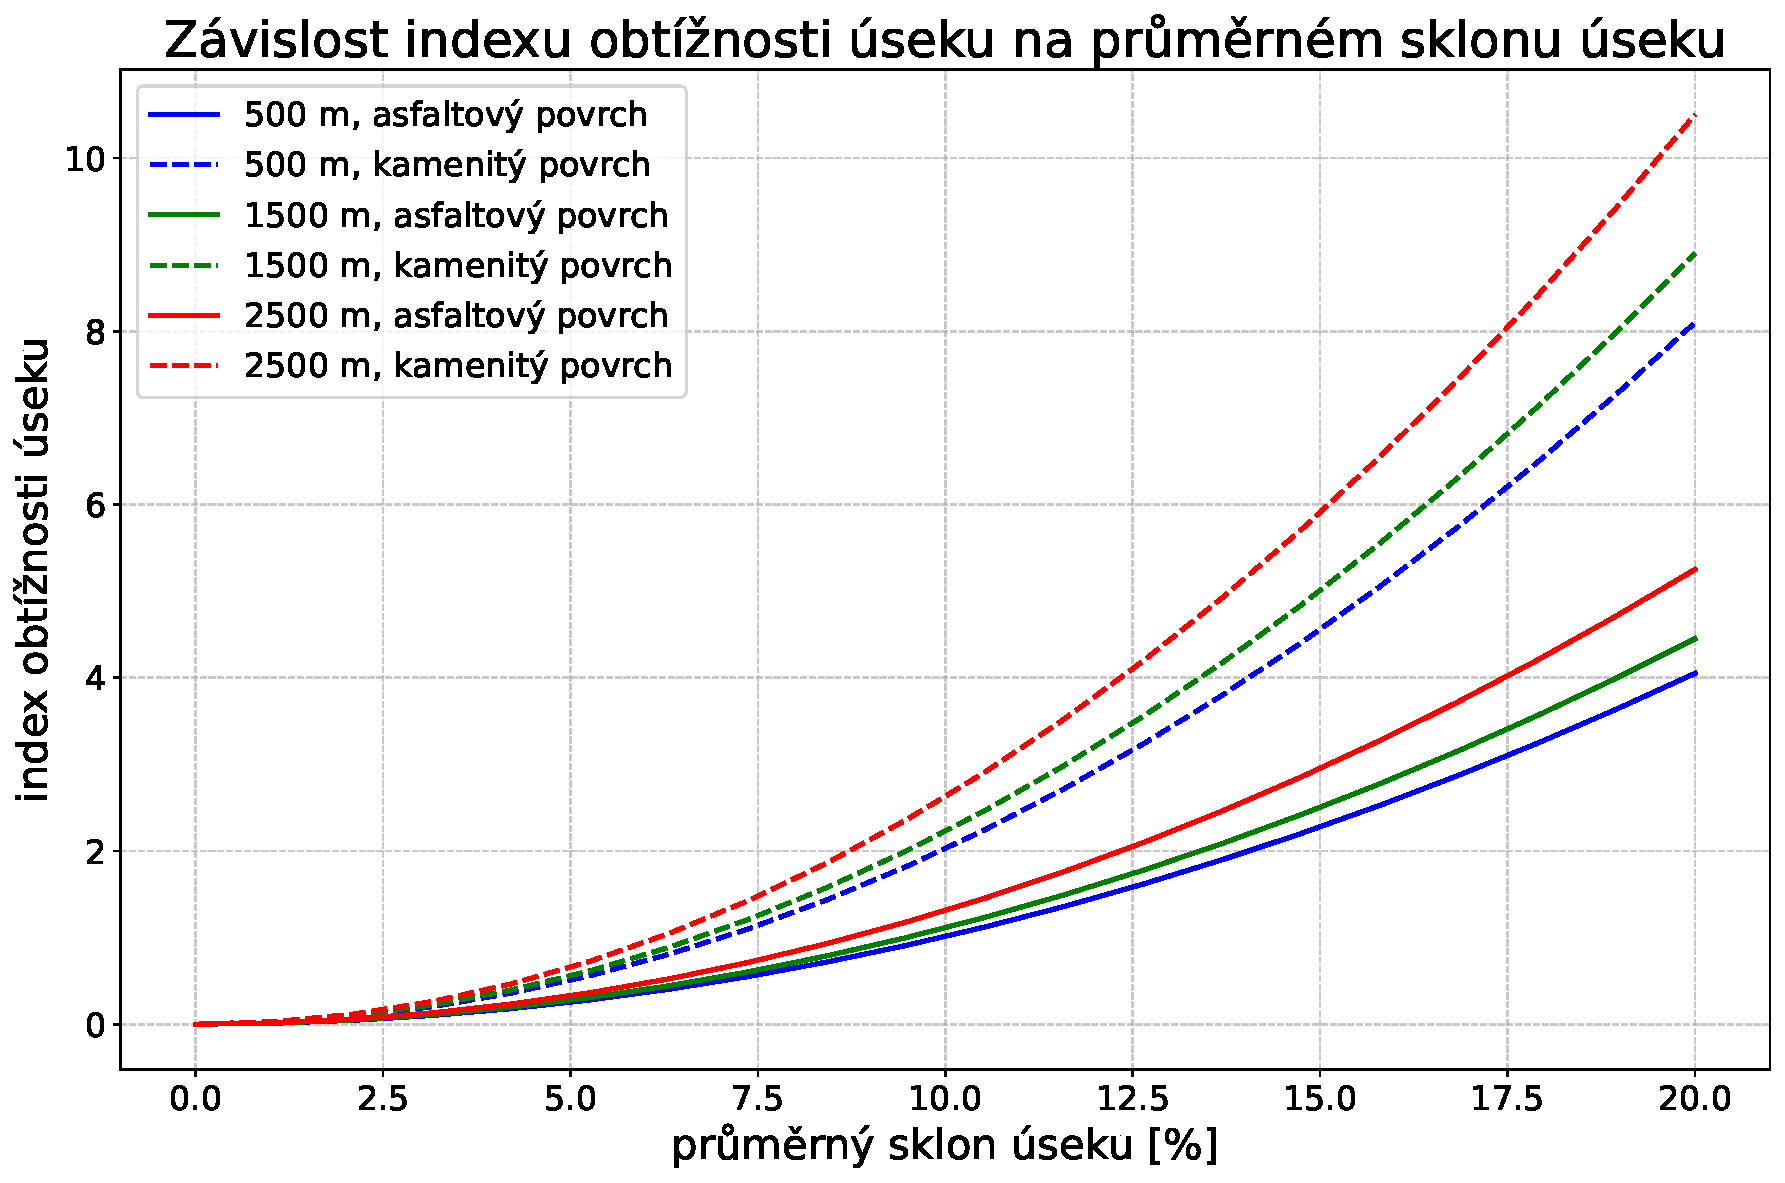
\includegraphics[width=\textwidth]{obrazky/difficulty-index.pdf}
    \caption[]{\textbf{Index obtížnosti části naplánovaných tras.} Grafické znázornění průběhu hodnot indexu náročnosti jednoho úseku trasy s~odpovídajícím průměrným sklonem pro vybrané průměrné nadmořské výšky a~druhy povrchu.}
    \label{DifficultyIndex}
\end{figure}

Ve spojení s~výškovými profily, podrobnými metrikami a~doplňujícími údaji, je celková obtížnost naplánovaných tras a~stoupání ve formě numerické klasifikace dalším zdrojem informací.
Číselný index náročnosti umožňuje sportovcům přímočaře a~efektivně porovnávat aktivity a~výkony mezi sebou.
Díky vybraným objektivním faktorům jsou veškeré trasy kategorizovány na základě shodného měřítka, což znamená snazší konfrontaci a~mnohem přínosnější analýzu.
Tento výstup má pochopitelně určitou výslednou hodnotu, kterou lze využít při plánování samotných sportovních výkonů a~zdolávání nových výzev.

\section{Význam a~využití objektivní klasifikace obtížnosti tras}
\label{the-importance-and-use-of-objective-route-difficulty-classification}

Matematický model vycházející z~podílu druhých mocnin průměrného sklonu a~délky úseku je rozšířen o~koeficienty reflektující průměrnou nadmořskou výšku a~různé typy povrchu.
Tyto faktory umožňují přesnější určení náročnosti, jelikož věrně odpovídají reálným podmínkám, se kterými se sportovci setkávají v~terénu.
Výsledný index obtížnosti tras tedy poskytuje komplexní a~objektivní ukazatel pro hodnocení různých aktivit a~zároveň možnost jejich vzájemného porovnání.

Hlavním přínosem této klasifikace je možnost efektivního plánování tras podle individuálních fyzických schopností a~sportovních cílů.
Uživatelé mohou na základě číselného ohodnocení snadno identifikovat trasy odpovídající jejich preferencím a~připravenosti.
Kromě toho je jednotné hodnocení užitečné i~pro srovnání výkonů mezi jednotlivými aktivitami, což umožňuje přesnější analýzu progresu.

Přestože prezentovaný model zohledňuje zásadní objektivní faktory ovlivňující fyzickou náročnost tras, v~budoucnu může být dále rozšířen o~další proměnné, například meteorologické podmínky nebo individuální fyziologické proporce sportovců.
Taková rozšíření mohou ještě více zpřesnit predikci reálné obtížnosti jednotlivých tras a~přispět k~jejich efektivnějšímu plánování.

\chapter{Analýza problému}
\label{problem-analysis}

Plánování tras je v~disciplínách, jako je cyklistika nebo turistika, klíčovým prvkem přípravy na fyzické aktivity.
Adekvátní volbu tras ovlivňují nejen sportovní výkony, ale i~bezpečnost a~celkové zážitky uživatelů.
Existuje řada nástrojů a~aplikací, které umožňují vyhledávání a~plánování tras, avšak jejich přístupy k~hodnocení obtížnosti se liší.

V~současné době není k~dispozici jednotný způsob určování náročnosti tras, který by uživatelům poskytoval srovnatelné informace.
Některé aplikace hodnotí trasy pouze na základě celkového převýšení, jiné zohledňují vzdálenost, či další parametry, ale žádný z~těchto přístupů neposkytuje komplexní hodnocení.
Tento nedostatek vede k~nejasnostem a~do jisté míry komplikuje plánování aktivit.

Aby bylo možné problém přesně definovat a~navrhnout efektivní řešení, je nutné nejprve analyzovat potřeby uživatelů a~identifikovat hlavní problémy současných metod hodnocení obtížnosti naplánovaných tras.
K~těmto účelům je vhodným zdrojem dat dotazníkový průzkum, který je využit pro sběr požadovaných informací.

\section{Analýza jednotlivých skupin potenciálních uživatelů}
\label{analysis-of-individual-groups-of-potential-users}

Podstatnou část uživatelů, kteří plánují trasy a~související náročné pasáže na základě jejich obtížnosti, tvoří zejména sportovci a~rekreační turisté.
Motivace mohou být jakékoliv, přičemž nejčastěji se jedná o~profesionální, či amatérské sportování a~volnočasovou zábavu.
Pouze malá část cyklistů využívá jízdní kola primárně jako dopravní prostředek.
Z~hlediska různých typů dominují horská kola, následovaná silničními, gravel a~krosovými koly.
Tyto odlišnosti ovlivňují požadavky na plánování tras a~preferované informace.

Hojně používanou službou pro plánování tras je webový mapový portál Mapy.cz, zatímco alternativní platformy jako Strava, Komoot nebo Cyclers jsou obecně zastoupeny minimálně.
Z~toho vyplývá, že výsledné řešení by mělo respektovat již zavedené zvyklosti uživatelů a~ideálně umožňovat import tras v~několika formátech, což značná většina preferuje jako hlavní způsob používání aplikace.
Mezi nejdůležitější parametry plánovaných tras a~dílčích úseků stoupání patří jejich celková vzdálenost, výškový profil, celkové převýšení a~počet nastoupaných metrů.
Přestože se potřeby jednotlivých skupin uživatelů mírně liší, všechny spojují požadavky na objektivní hodnocení náročnosti tras a~snadnou interpretaci získaných údajů prostřednictvím grafických vizualizací.

Elementární požadavky vychází z~ověřených metod, kterými uživatelé používají podobné aplikace zaměřené na plánování a~vizualizace.
Všeobecně lze za téměř povinné nároky označit přítomnost výškových profilů naplánovaných tras, scházet by však neměly ani klasické statistiky v~podobě číselných hodnot.
Řada sportovců by jistě ocenila detailní grafická zpracování a~vizualizace náročných úseků stoupání.
S~většinou uvedených potřeb souvisí nutnost využití dostatečně přesných mapových datových sad s~relevantími informacemi nejen o~zeměpisných šířkách a~délkách, ale také nadmořských výškách.
Vlastní prezentace výsledků naopak vyžadují adekvátní nastavení patřičných hranic filtračních metod k~úpravě výškových profilů a~efektivní algoritmy, které slouží k~validaci průběhu tras a~nadmořských výšek.

Uživatelské rozhraní výsledného řešení by mělo být intuitivní ve smyslu pokročilé a~zároveň snadné orientace.
Hlavním úkolem je redukce nezbytně nutných kroků na samotné plánování tras, export těchto vstupních dat do souborů požadovaných formátů a~jejich nahrání do aplikace pro vygenerování analýzy.
Současně jsou zamýšleny další případy užití, například uložení již naplánovaných aktivit do oblíbených.
Při používání aplikace by neměla být vyžadována registrace a~jakékoliv výjimečné postupy, aby bylo řešení zpřístupněno co největšímu množství zájemců.

\section{Definice problémů}
\label{problem-definition}

Na základě analýzy potřeb uživatelů a~momentálního stavu hodnocení tras je možné identifikovat klíčové problémy, které je třeba řešit.
Adekvátní zvládnutí těchto překážek může vést k~odpovídajícímu návrhu, který bude zohledňovat uživatelské nároky v~přijatelné kvalitě.
Detailní průzkum existujících aplikací a~služeb, stejně jako vyhodnocení odpovědí potenciálních uživatelů, doplňuje kompletní zadání problému a~definuje veškeré podstatné maličkosti k~pozdější implementaci.

\subsection{Problém nejednotnosti hodnocení obtížnosti}
\label{the-problem-of-inconsistency-in-difficulty-ratings}

Současné aplikace používají různé metody k~určování obtížnosti tras a~dílčích náročných segmentů stoupání.
Některé berou v~úvahu pouze převýšení, jiné zahrnují sklon nebo délku tras, ale žádný systém nenabízí komplexní přístup.
Tato nejednotnost vede k~tomu, že stejné aktivity mohou být v~různých aplikacích hodnoceny zcela odlišně, což uživatelům komplikuje plánování.
Samostatným fenoménem jsou různé typy povrchů, které mají zásadní vliv na fyzickou náročnost.
Asfaltové silnice umožňují plynulý pohyb, zatímco kamenité stezky a~traily vyžadují daleko větší úsilí.
Stávající metody však často povrchy nezohledňují, což vede k~nepříliš přesným hodnocením obtížnosti.

Změny, průměrné a~maximální hodnoty nadmořských výšek ovlivňují koncentrace kyslíku ve vzduchu, a~tím rovněž náročnost naplánovaných aktivit.
Stejně tak dvě trasy s~identickým souhrnným převýšením mohou mít různou obtížnost v~závislosti na tom, jak jsou stoupání rozložena.
Prudké úseky vyžadují pochopitelně jiný přístup a~taktiku než dlouhá, táhlá a~mírná stoupání.
Každý sportovec má navíc jinou úroveň fyzické kondice a~obtížnost aktivit může být vnímána odlišně.
Aby bylo možné porovnávat trasy objektivně, je třeba definovat metodu, která bude založena na měřitelných parametrech nezávislých na individuální kondici uživatelů.

\subsection{Problém nedostatku detailních vizualizací stoupání}
\label{the-problem-of-lack-of-detailed-visualisations-of-climbs}

Více než 85\,\%~respondentů by ocenilo detailní grafickou vizualizaci úseků stoupání.
Současná řešení, jako Mapy.cz nebo Komoot, zobrazují základní výškový profil, ale neposkytují podrobné informace o~klíčových faktorech včetně maximálního a~průměrného sklonu, nejstrmějších úseků nebo hodnocení obtížnosti.
Navíc většina dotázaných uvedla, že by jim detailní vizualizace pomohla lépe rozvrhnout fyzické síly a~přizpůsobit tempo jízdy.
To znamená, že lepší grafické zobrazení a~kvalitnější interpretace důležitých aspektů aktivit může přímo přispět ke komfortnějším a~efektivnějším výjezdům.

\subsection{Problém omezených možností integrace a~práce s~trasami}
\label{the-problem-of-limited-integration-options-and-working-with-routes}

Existující aplikace často neumožňují dostatečně personalizovat naplánované cyklotrasy.
Velká většina by ocenila možnost ukládat si trasy do oblíbených a~nezanedbatelné množství uživatelů by si přálo přidávat vlastní poznámky nebo média k~jednotlivým úsekům.
Tato funkcionalita by umožnila lepší archivaci tras a~jejich zpětné analýzy.
Co se týče integrace, většina sportovců preferuje plánování tras pomocí externích služeb, mezi které jistě patří mnohokrát zmíněné Mapy.cz, Strava či Komoot, a~následné nahrání souboru se vstupními daty do aplikace k~vygenerování podrobné analýzy.
Z~toho vyplývá, že nové řešení by nemělo konkurovat těmto zavedeným platformám, ale mělo by se soustředit primárně na dodatečnou analýzu a~vizualizaci.

\section{Definice požadavků}
\label{requirements-definition}

Na základě identifikovaných problémů lze definovat klíčové požadavky na výsledné řešení.
Realizací následujících návrhů by měla vzniknout platforma, která zaplní chybějící místo v~nabídce aplikací určených pro plánování, analýzy a~grafické vizualizace sportovních aktivit.

\begin{itemize}
    \item \textbf{Detailní vizualizace stoupání.}
    Grafická reprezentace úseků s~důrazem na celkovou vzdálenost, celkové převýšení, průměrný a~maximální sklon a~nejstrmější pasáže.
    Možnost podrobných vizualizací by jistě zvýšila použitelnost.
    \item \textbf{Jednoduché a~intuitivní uživatelské rozhraní.}
    Uživatelé preferují přehledné řešení, které nevyžaduje složité nastavení.
    Zároveň je však nutné zpřístupnit všechny důležité funkce kompaktně a~srozumitelně na jednom místě.
    \item \textbf{Možnost ukládání a~správy tras.}
    Uživatelé by měli mít možnost uložit si oblíbené trasy a~analyzované úseky.
    Tímto způsobem si mohou sportovci vzájemně porovnávat naplánované trasy mezi sebou a~procházet si dříve vygenerované analýzy a~vizualizace.
    \item \textbf{Integrace s~existujícími platformami.}
    Možnost nahrání vstupních dat v~rámci různých typů souborů k~dodatečné analýze.
    Podpora širšího spektra formátů geografických dat poskytuje mnohem větší variabilitu s~již využívanými aplikacemi.
    \item \textbf{Mobilní aplikace a~webová stránka jako preferovaná forma řešení.}
    Většina respondentů dotazníkového průzkumu by upřednostňovala nejen mobilní aplikaci, ale také webovou stránku.
    Tento přístup zajistí požadovanou přenositelnost mezi platformami a~tím pádem i~mnohem větší uživatelskou základnu.
\end{itemize}

\chapter{Návrh řešení}
\label{design-of-the-solution}

Na základě provedené analýzy je navrženo řešení, které by mělo sloužit především k~objektivnímu ohodnocení obtížnosti naplánovaných výjezdů včetně nejdůležitějších statistik či náročných pasáží.
Pro jednodušší a~srozumitelnější pochopení velkého množství metrik a~údajů jsou zvoleny odpovídající grafické vizualizace a~prezentace přesného průběhu tras na mapovém podkladu.
Postup plánování cyklistických výletů funguje v~současnosti na několika platformách poměrně spolehlivě.
Smyslem navrženého řešení není konkurovat uvedeným nástrojům, ale podpořit hlubší analýzu tras před jejich vlastním absolvováním.
Vzhledem na uživatelské a~technické požadavky směřuje návrh řešení k~mobilní aplikaci, kterou je v~případě potřeby možné zobrazit rovněž ve webovém prohlížeči.
Ilustrační obrázky v~této kapitole jsou vytvořeny pomocí nástrojů draw.io\footnote{draw.io diagram software --~více viz \url{https://app.diagrams.net}.}, Figma\footnote{Figma: The Collaborative Interface Design Tool --~více viz \url{https://www.figma.com}.} a~mapových podkladů OpenStreetMap\footnote{Přispěvatelé OpenStreetMap (OSM) --~více viz \url{https://www.openstreetmap.org}.}.

\section{Architektura}
\label{architecture}

Aplikace je navržena jako vícevrstvá klient--server architektura, kde se jednotlivé části zaměřují na konkrétní odpovědnosti v~systému s~cílem zajistit modularitu, přehlednost a~snadnou udržovatelnost.
Architektonické řešení rozlišuje zejména serverovou a~prezentační vrstvu.
Klientská část je odpovědná za interakci s~uživateli, umožňuje načítání datových vstupů, zobrazení výstupů analýzy, vizualizace a~správu obsahu.
Celkový návrh architektury aplikace je na obrázku \ref{Architecture}.

\begin{figure}[ht]
    \centering
    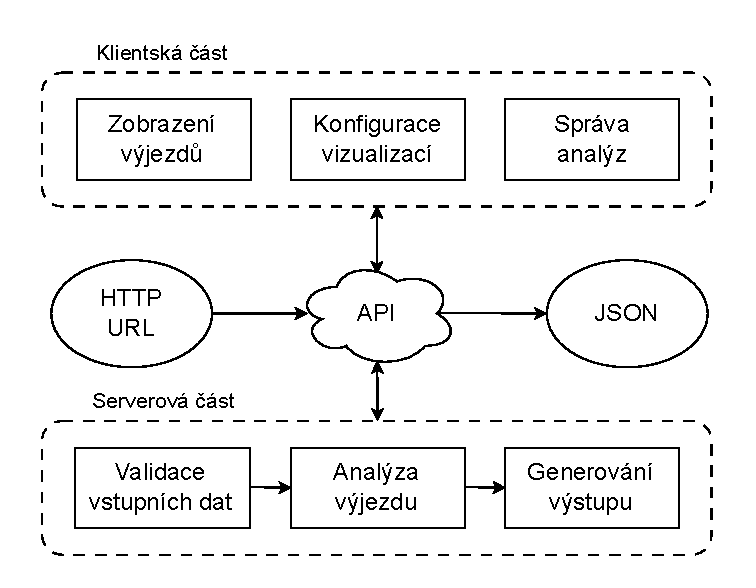
\includegraphics[width=\textwidth]{obrazky/architecture.pdf}
    \caption[]{\textbf{Schéma návrhu architektury aplikace.} Návrh architektury aplikace rozdělené na klientskou a~serverovou část, které mezi sebou komunikují prostřednictvím API.}
    \label{Architecture}
\end{figure}

Základním stavebním kamenem jsou samotné zevrubné analýzy vstupních dat.
V~případě úspěšné validace geografického souboru mají uživatelé možnost zobrazit si nejdůležitější statistiky aktivit, přesné itineráře stop na mapovém podkladu nebo nejnáročnější segmenty.
Používání aplikace není limitováno registrací, tudíž i~nepřihlášení uživatelé si mohou nechat vygenerovat pokročilé analýzy bez omezení.
Současně však mají možnost si již vytvořené výlety se všemi podrobnostmi a~vizualizacemi uložit do oblíbených pro pozdější správu tras.

Na základě provedeného průzkumu je zvoleno přehledné zobrazení, kde jsou všechny podstatné funkce na dosah.
Obrázek \ref{UserInterface}~znázorňuje návrh grafického uživatelského rozhraní jedné obrazovky aplikace.
Úvodní obrazovka obsahuje formulář pro import geografických souborů a~následující krok slouží ke kontrole skutečného obsahu vstupních dat a~vlastnímu generování odpovídajících numerických i~grafických výstupů.
Výslednou podobu grafických vizualizací si mohou uživatelé s~předstihem do jisté míry přizpůsobit vlastním potřebám na obrazovce s~nastavením, která je rovněž snadno přístupná z~globálního navigačního menu.

\begin{figure}[ht]
    \centering
    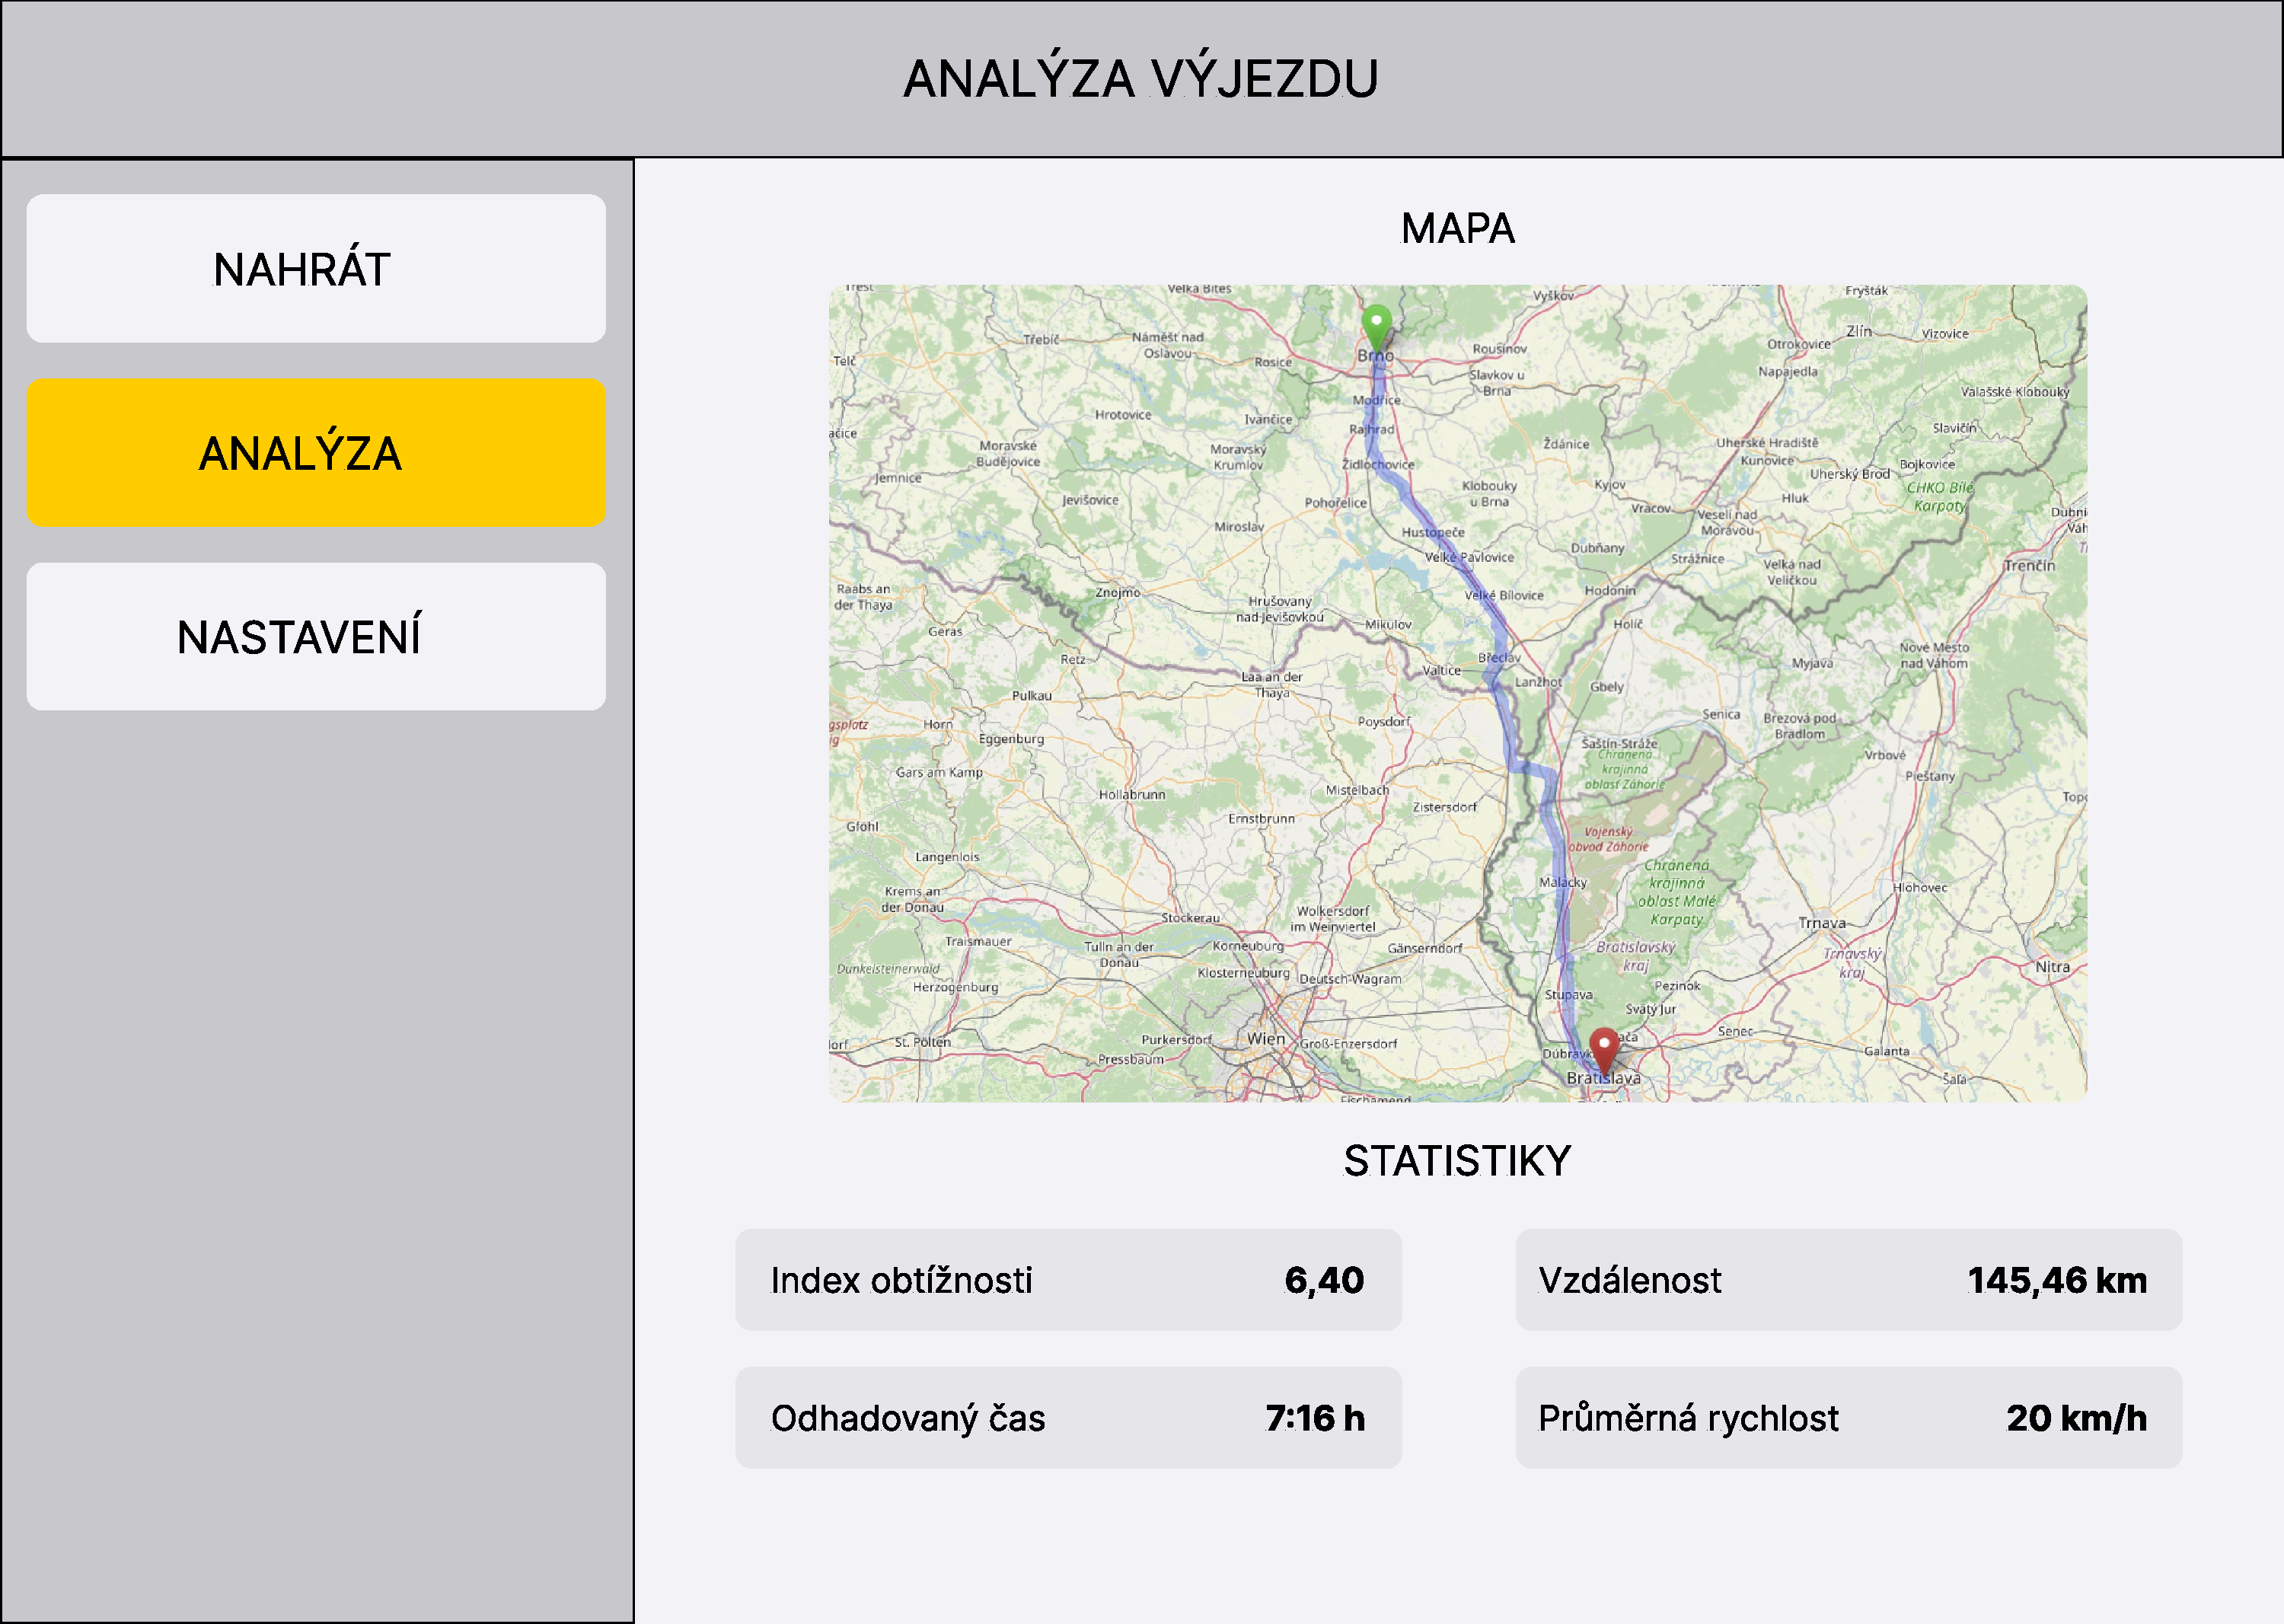
\includegraphics[width=\textwidth]{obrazky/user-interface.pdf}
    \caption[]{\textbf{Grafické uživatelské rozhraní.} Návrh grafického uživatelského rozhraní jedné specifické obrazovky aplikace, která slouží k~analýze naplánovaných cyklistických výjezdů a~prezentaci výstupů.}
    \label{UserInterface}
\end{figure}

\section{Datový model a~struktura systému}
\label{data-model-and-system-structure}

Použitý model odpovídá klasické oddělené architektuře klient--server s~využitím API\footnote{Application Programming Interface (API) -- více viz \url{https://en.wikipedia.org/wiki/API}.}.
Klientská část se stará výhradně o~prezentaci dat, interakci s~uživateli a~zajištění responzivního zobrazení obsahu.
Veškeré výpočetně náročné nebo datově orientované operace jsou delegovány na server, který je vystaven jako sada koncových bodů API, s~nimiž si zařízení vyměňují informace prostřednictvím počítačové sítě.
Ačkoliv je koncipován jako samostatná služba, jeho účelem je poskytovat konkrétní funkcionalitu navržené aplikaci, nejedná se tedy o~plnohodnotný server.

Tento přístup přináší několik klíčových výhod, mezi které patří flexibilita vývoje s~možností nezávislého nasazení klientské a~serverové části.
Totožný server může být využit i~jinými klienty v~podobě mobilních, či webových aplikací.
Dalším benefitem je jistě horizontální škálovatelnost jedné části aplikace bez vynuceného zásahu do druhé části.
Komunikace mezi klienty a~serverem probíhá formou protokolu HTTP\footnote{Hypertext Transfer Protocol (HTTP) -- více viz \url{https://en.wikipedia.org/wiki/HTTP}.}, konkrétně pomocí adekvátních požadavků s~přiloženými metadaty.
Server na základě přijatých požadavků spustí analýzu, jejíž výsledky a~výstupy následně odešle v~předem daných formátech zpět klientovi, který aktualizuje stav aplikace a~zobrazí příslušný obsah.

Nástroj je navržen takovým způsobem, že veškerá nezbytně nutná data lze získat ze vstupních geografických souborů, které mají validní obsah.
Při využití vhodných knihoven jsou jediným požadavkem korektní záznamy zeměpisných souřadnic a~nadmořských výšek.
Doplňující údaje, jako např. počet nastoupaných a~sestoupaných metrů, průměrný a~maximální sklon nebo další zajímavosti, je poté možné přiřadit k~jednotlivým zeměpisným bodům.
Značná část výstupů je však reprodukována vizuálně, či jiným grafickým způsobem.

\section{Elementární funkcionalita aplikace}
\label{elementary-application-functionality}

Proces generování analýzy naplánovaných cyklistických tras zahrnuje několik po sobě jdoucích a~zároveň na sebe logicky navazujících kroků:

\begin{itemize}
    \item \textbf{Naplánování sportovní aktivity a~vytvoření geografického souboru.}
    Jedná se o~povinnou prerekvizitu celého procesu generování analýzy.
    Tuto akci není možné provést přímo v~navržené aplikaci, nicméně v~současnosti existuje velký počet služeb s~tímto zaměřením, více viz sekce \ref{available-geographic-data-suitable-for-cycle-routes-analysis}.
    Vytvořený geografický soubor obsahuje požadovaná data, která již mohou být považována za data vstupní.
    \item \textbf{Nahrání vstupního geografického souboru.}
    Hlavní obrazovka nástroje slouží k~jedinému úkonu, kterým je výběr vstupních dat z~úložiště místního zařízení a~jejich import do aplikace.
    Jelikož hlavním účelem řešení je generování detailní analýzy, je možné nahrávat soubory do aplikace jednotlivě.
    Zároveň je postup výběru souboru omezen pouze na podporované formáty FIT, GPX, KML a~TCX.
    \item \textbf{Přizpůsobení vzhledu výstupní grafické vizualizace.}
    Volitelný krok, který je pro korektní funkčnost nutné vykonat před samotným spuštěním procesu generování analýzy.
    Nastavení se týká především použité délky kroku jednotlivých výpočetních algoritmů zajišťujících přesnosti statistik, zobrazení náročných pasáží s~určitou minimální obtížností nebo volby požadovaných jednotek.
    \item \textbf{Uložení vygenerované analýzy do oblíbených.}
    Pokud je požadovaná analýza vygenerována úspěšně a~uživatelé jsou s~vizualizacemi a~statistikami spokojeni, mohou být tyto výstupy označeny jako oblíbené, což ve výsledku znamená snazší a~daleko rychlejší přístup k~těmto datům v~budoucnu.
\end{itemize}

\subsection{Naplánování sportovní aktivity a~vytvoření geografického souboru}
\label{planning-sports-activities-and-creating-geographic-files}

Zcela nezbytným předpokladem pro práci s~aplikací je vlastnictví validního geografického souboru, který reprezentuje plánovaný výjezd, trasu, nebo zaznamenanou sportovní aktivitu.
Tento soubor vzniká nejčastěji exportem ze specializovaných platforem, jako jsou například Komoot, Mapy.cz, Ride with GPS nebo Strava.
Soubor musí obsahovat posloupnost zeměpisných souřadnic, popřípadě dalších metadat včetně nadmořských výšek, časových údajů či maximálních a~minimálních hodnot.
Aplikace následně tato data využívá k~výpočtu klíčových statistik a~k~vizualizaci výškových profilů stop.
Samotné řešení touto funkcionalitou nedisponuje a~probíhá tedy zcela mimo v~režii uživatelů.

\subsection{Nahrání vstupního geografického souboru}
\label{uploading-input-geographic-files}

Po spuštění nástroje je uživatelům zobrazena výchozí obrazovka s~možností importu geografického souboru ze zařízení.
Podporovány jsou formáty FIT, GPX, KML a~TCX, které patří k~nejpoužívanějším v~oblasti záznamu a~sdílení sportovních aktivit.
Po výběru souboru dochází k~jeho nahrání a~odeslání na server, kde proběhne kontrola a~předzpracování dat.
Validace vstupu hraje klíčovou roli --~zajišťuje, že nadcházející výpočty budou přesnější, a~eliminuje rizika spojená s~chybnou interpretací dat.
Jakmile proběhne vše úspěšně, je možné přejít ke generování výstupů.
Pokud však vstupní data neobsahují dostatečné informace, jsou uživatelé na tuto skutečnost upozorněni.

\subsection{Přizpůsobení vzhledu výstupní grafické vizualizace}
\label{customizing-the-appearance-of-output-graphic-visualizations}

Vzhledem k~tomu, že cílem aplikace je prezentace velkého množství dat, je důležité umožnit uživatelům přizpůsobení vizuálního výstupu.
Tato funkcionalita zvyšuje použitelnost nástroje napříč různými potřebami.
Uživatelé mohou provádět nastavení minimální hodnoty indexu obtížnosti, který určuje to, jaká stoupání jsou později zahrnuta v~detailní vizualizaci.
Mimo jiné lze nastavit rovněž metrické, nebo imperiální jednotky.
Změny vzhledu lze upravovat v~nastavení aplikace a~při generování analýzy se automaticky aplikují.
Díky tomu mají uživatelé plnou kontrolu nad tím, jak budou data prezentována, a~to bez nutnosti dodatečných úprav.

\subsection{Uložení vygenerované analýzy do oblíbených}
\label{saving-and-exporting-generated-analyses-to-favorites}

Po úspěšném dokončení procesu tvorby analýzy si mohou uživatelé výsledky uložit mezi oblíbené položky.
Tímto krokem se usnadní proces potenciálního vzájemného porovnání naplánovaných cyklistických tras mezi sebou, totéž platí také pro náročné úseky stoupání.
Rychlý přístup ke statistikám je poté možný bez nutnosti opakovaného importu vstupních geografických dat ze zdrojového souboru.
Správa dříve vytvořených tras přispívá k~vyšší efektivitě při opakovaném používání aplikace.
Kromě ukládání je k~dispozici také možnost exportu v~podobě jednotlivých grafů.
Export usnadňuje další práci s~daty mimo rozhraní aplikace, například pro sdílení nebo publikování.

\chapter{Implementace}
\label{implementation}

V~této kapitole je popsána implementační část navrženého řešení.
Nejprve jsou představeny použité technologie a~nástroje, následně jsou jednotlivé části aplikace rozebrány z~hlediska jejich funkce.
Důraz je kladen na klíčové aspekty vývoje, jako je architektura aplikace, struktura kódu a~řešení složitějších částí vlastní realizace nástroje.

\section{Použité technologie}
\label{technologiew-used}

Pro vývoj aplikace je zvolena sada technologií, které reflektují požadavky na multiplatformní přístup, efektivní zpracování geografických dat a~jednoduchou správu výsledků.
Klíčovými aspekty při výběru technologií je jejich stabilita, jednoduchost uživatelského rozhraní a~schopnost bezproblémové integrace jednotlivých komponent do jediného komplexního řešení.

Klientská část nástroje je realizována pomocí aplikačního frameworku Flutter\footnote{Aplikační framework Flutter --~více viz \url{https://flutter.dev}.}, který umožňuje vývoj nativně kompilovaných mobilních a~webových aplikací z~jediného zdrojového kódu.
Zvolen je především kvůli své flexibilitě, poměrně vysokému výkonu a~podpoře vývoje pro více platforem současně.
Jazykem použitým při vývoji prezentační vrstvy je Dart\footnote{Programovací jazyk Dart --~více viz \url{https://dart.dev}.}, který je považován za nedílnou součást Flutteru.
Díky své reaktivní architektuře umožňuje Flutter snadnou implementaci uživatelského rozhraní a~rychlou odezvu aplikace na změny aktuálního stavu.

Serverová část aplikace je implementována v~jazyce Python s~využitím webového rámce FastAPI\footnote{Webový rámec FastAPI --~více viz \url{https://fastapi.tiangolo.com}.}, který je určen pro tvorbu moderních rozhraní služeb API založených na protokolu HTTP.
Tato technologie je zvolena zejména díky své jednoduchosti, rychlosti a~přirozené podpoře asynchronního zpracování příchozích požadavků.
Mezi další výhody této volby patří široká škála knihoven zaměřených na výpočty a~práci s~geografickými daty, jako jsou \texttt{matplotlib}, \texttt{numpy} nebo \texttt{pandas}.
Tyto knihovny jsou využívány pro analýzu a~zpracování vstupních dat, stanovení klíčových statistik a~generování grafických výstupů v~podobě výškových profilů.

\section{Architektura aplikace}
\label{application-architecture}

Základní struktura aplikace vychází z~navrženého řešení a~jedná se tedy o~vícevrstvou klient--server architekturu.
Většina logiky je rozdělena odpovídajícím způsobem mezi klientskou část implementovanou ve frameworku Flutter a~serverovou část, která je postavena na FastAPI.
Řídicím prvkem aplikace je prezentační vrstva, která zobrazuje uživateli aktuální stav systému, třebaže žádným způsobem nemanipuluje s~interními daty.

\subsection{Klientská část}
\label{client-section}

Samotná klientská část se skládá ze dvou hlavních vrstev, jak ilustruje obrázek \ref{ClientArchitecture}.
Stav proudí z~datové vrstvy směrem k~uživatelskému rozhraní, zatímco události směřují opačně, z~prezentační vrstvy zpět do datové vrstvy.
Ačkoliv se v~mnoha aplikacích nachází třetí logická vrstva, v~rámci navrženého řešení jsou dostačující dvě hlavní vrstvy, jelikož veškeré výpočetně náročné operace nad daty probíhají vzdáleně na serverové části.
Využití logické vrstvy tedy není nezbytně nutné, jelikož klientská část neobsahuje složitou výpočetní logiku.

\begin{itemize}
    \item \textbf{Vrstva uživatelského rozhraní.}
    Uživatelské rozhraní je v~rámci frameworku Flutter tvořeno komponenty zvanými widgety.
    Úlohou uživatelského rozhraní je zpracování interakce s~uživatelem a~zobrazení aktuálního stavu dat, které poskytuje datová vrstva.
    \item \textbf{Datová vrstva.} Datová vrstva spravuje interakce se zdroji dat, vystavuje data a~metody vrstvě uživatelského rozhraní a~uchovává aktuální stav systému.
\end{itemize}

\begin{figure}[ht]
    \centering
    
\includegraphics[width=\textwidth]{obrazky/mvvm-intro-with-layers.png}
    \caption[]{\textbf{Architektonický vzor klientské části aplikace.} Oddělení aktuálního stavu od uživatelského rozhraní, které tento stav zobrazuje.\footnotemark}
    \label{ClientArchitecture}
\end{figure}

\footnotetext{Převzato z: \url{https://docs.flutter.dev/assets/images/docs/app-architecture/guide/mvvm-intro-with-layers.png}.}

Z~hlediska vlastní implementace je klientská část aplikace navržena jako reaktivní rozhraní využívající stavové řízení prostřednictvím tzv. poskytovatelů, které slouží jako prostředník mezi datovou a~prezentační vrstvou.
Tyto třídy uchovávají aktuální stav aplikace a~umožňují jeho centrální správu, přičemž při jakékoliv změně hodnot informují všechny komponenty, které jsou na daných datech závislé.
Tím je zajištěna automatická aktualizace uživatelského rozhraní bez nutnosti manuálního přepočítávání nebo překreslování jednotlivých částí.

Aplikace je inicializována ve funkci \texttt{main}, kde dochází ke spuštění hlavního widgetu a~nastavení jednotlivých poskytovatelů.
Tento přístup umožňuje sdílení dat v~rámci celé aplikace a~zároveň odděluje samostatné funkční oblasti.
Základní rozvržení a~navigace mezi částmi aplikace je řešena pomocí dynamického zobrazení aktuálně vybrané stránky podle polohy v~navigačním menu.
Architektonicky se aplikace drží jednoduchého, ale funkčního návrhu, v~němž každá stránka aplikace existuje ve dvou verzích, které se zobrazují na základě aktuální šířky obrazovky.
Toto responzivní chování přispívá ke zlepšení uživatelského zážitku napříč různými zařízeními, aniž by bylo nutné vytvářet samostatné aplikace.

\subsection{Serverová část}
\label{server-section}

Serverová část nástroje je implementována jako REST\footnote{Representational State Transfer (REST) --~více viz \url{https://en.wikipedia.org/wiki/REST}.} API založené na moderním frameworku FastAPI.
Hlavním úkolem této vrstvy je zpracování geografických dat odeslaných z~klientské aplikace, jejich důkladná analýza a~zpětné vrácení výsledků ve formě statistických výstupů a~grafických vizualizací.
Tímto způsobem je dosaženo oddělení výpočetně náročných operací od uživatelského rozhraní, čímž se významně snižuje zátěž na koncových zařízeních.

Server přijímá požadavky v~podobě nahraných geografických souborů v~předem stanovených formátech, které obsahují informace o~naplánovaných cyklistických výjezdech.
Po přijetí těchto souborů dochází k~jejich načtení, analýze a~převedení do strukturované formy vhodné pro další zpracování.
Z~takto připravených vstupních dat jsou následně vypočítány nejrůznější statistiky, jako jsou celková vzdálenost, převýšení, počet nastoupaných a~sestoupaných metrů, identifikace náročných úseků stoupání či objektivní index obtížnosti.
Tyto hodnoty jsou následně zformátovány do výstupního objektu JSON\footnote{JavaScript Object Notation (JSON) --~více viz \url{https://www.json.org/json-en.html}.}, který je vrácen zpět klientovi.
Součástí serveru je rovněž generování grafických vizualizací, především výškových profilů, které jsou ukládány jako obrázky do paměti.
Pro zachování možnosti jejich jednoduchého zobrazení na klientské straně je nutné obsah serializovat dle standardizovaných formátů, a~to bez nutnosti ukládání na disk nebo použití dalších služeb.

Serverová logika je navržena tak, aby byla co nejvíce soběstačná a~nezávislá na kontextu klienta.
Všechny výpočty a~odvozené metriky jsou prováděny výhradně na základě vstupních dat a~parametrů zaslaných klientem.
Díky tomu je možné rozšíření funkcionality bez nutnosti zásahu do samotné klientské vrstvy.
Z~hlediska zabezpečení a~přístupu je server nakonfigurován tak, aby umožňoval požadavky z~různých domén, což usnadňuje jeho integraci nejen do mobilních, ale i~webových aplikací.

\section{Implementace elementární funkcionality}
\label{implementation-of-elementary-functionalities}

Elementární funkcionality tvoří jádro celé aplikace, popisované části vycházejí z~návrhu uvedeného v~sekci \ref{elementary-application-functionality} a~pokrývají implementaci složitějších procesů na serverové i~klientské straně.
Každá funkcionalita se pochopitelně skládá z~dalších podpůrných funkcí, které ve výsledku představují celkové chování aplikace.

\subsection{Nahrání a~zpracování vstupního souboru}
\label{uploading-and-processing-input-files}

Uživatelské rozhraní na klientské straně poskytuje jednoduchý, avšak robustní způsob výběru geografického souboru, který je znázorněn na obrázku \ref{DefaultScreen}.
K~tomuto účelu je využita komponenta \texttt{FilePicker}, která umožňuje výběr pouze podporovaných formátů FIT, GPX, KML a~TCX.
Přestože je na straně klienta omezen výběr vstupních dat na uvedené typy souborů, serverová vrstva provádí před vlastními analýzami další nezbytné kontroly skutečného obsahu pro pozdější správnou interpretaci geografických dat.
Podmínkou pro pokračování v~analýze je, aby byl soubor lokálně uložen a~nebyl poškozen.

\begin{figure}[ht]
    \centering
    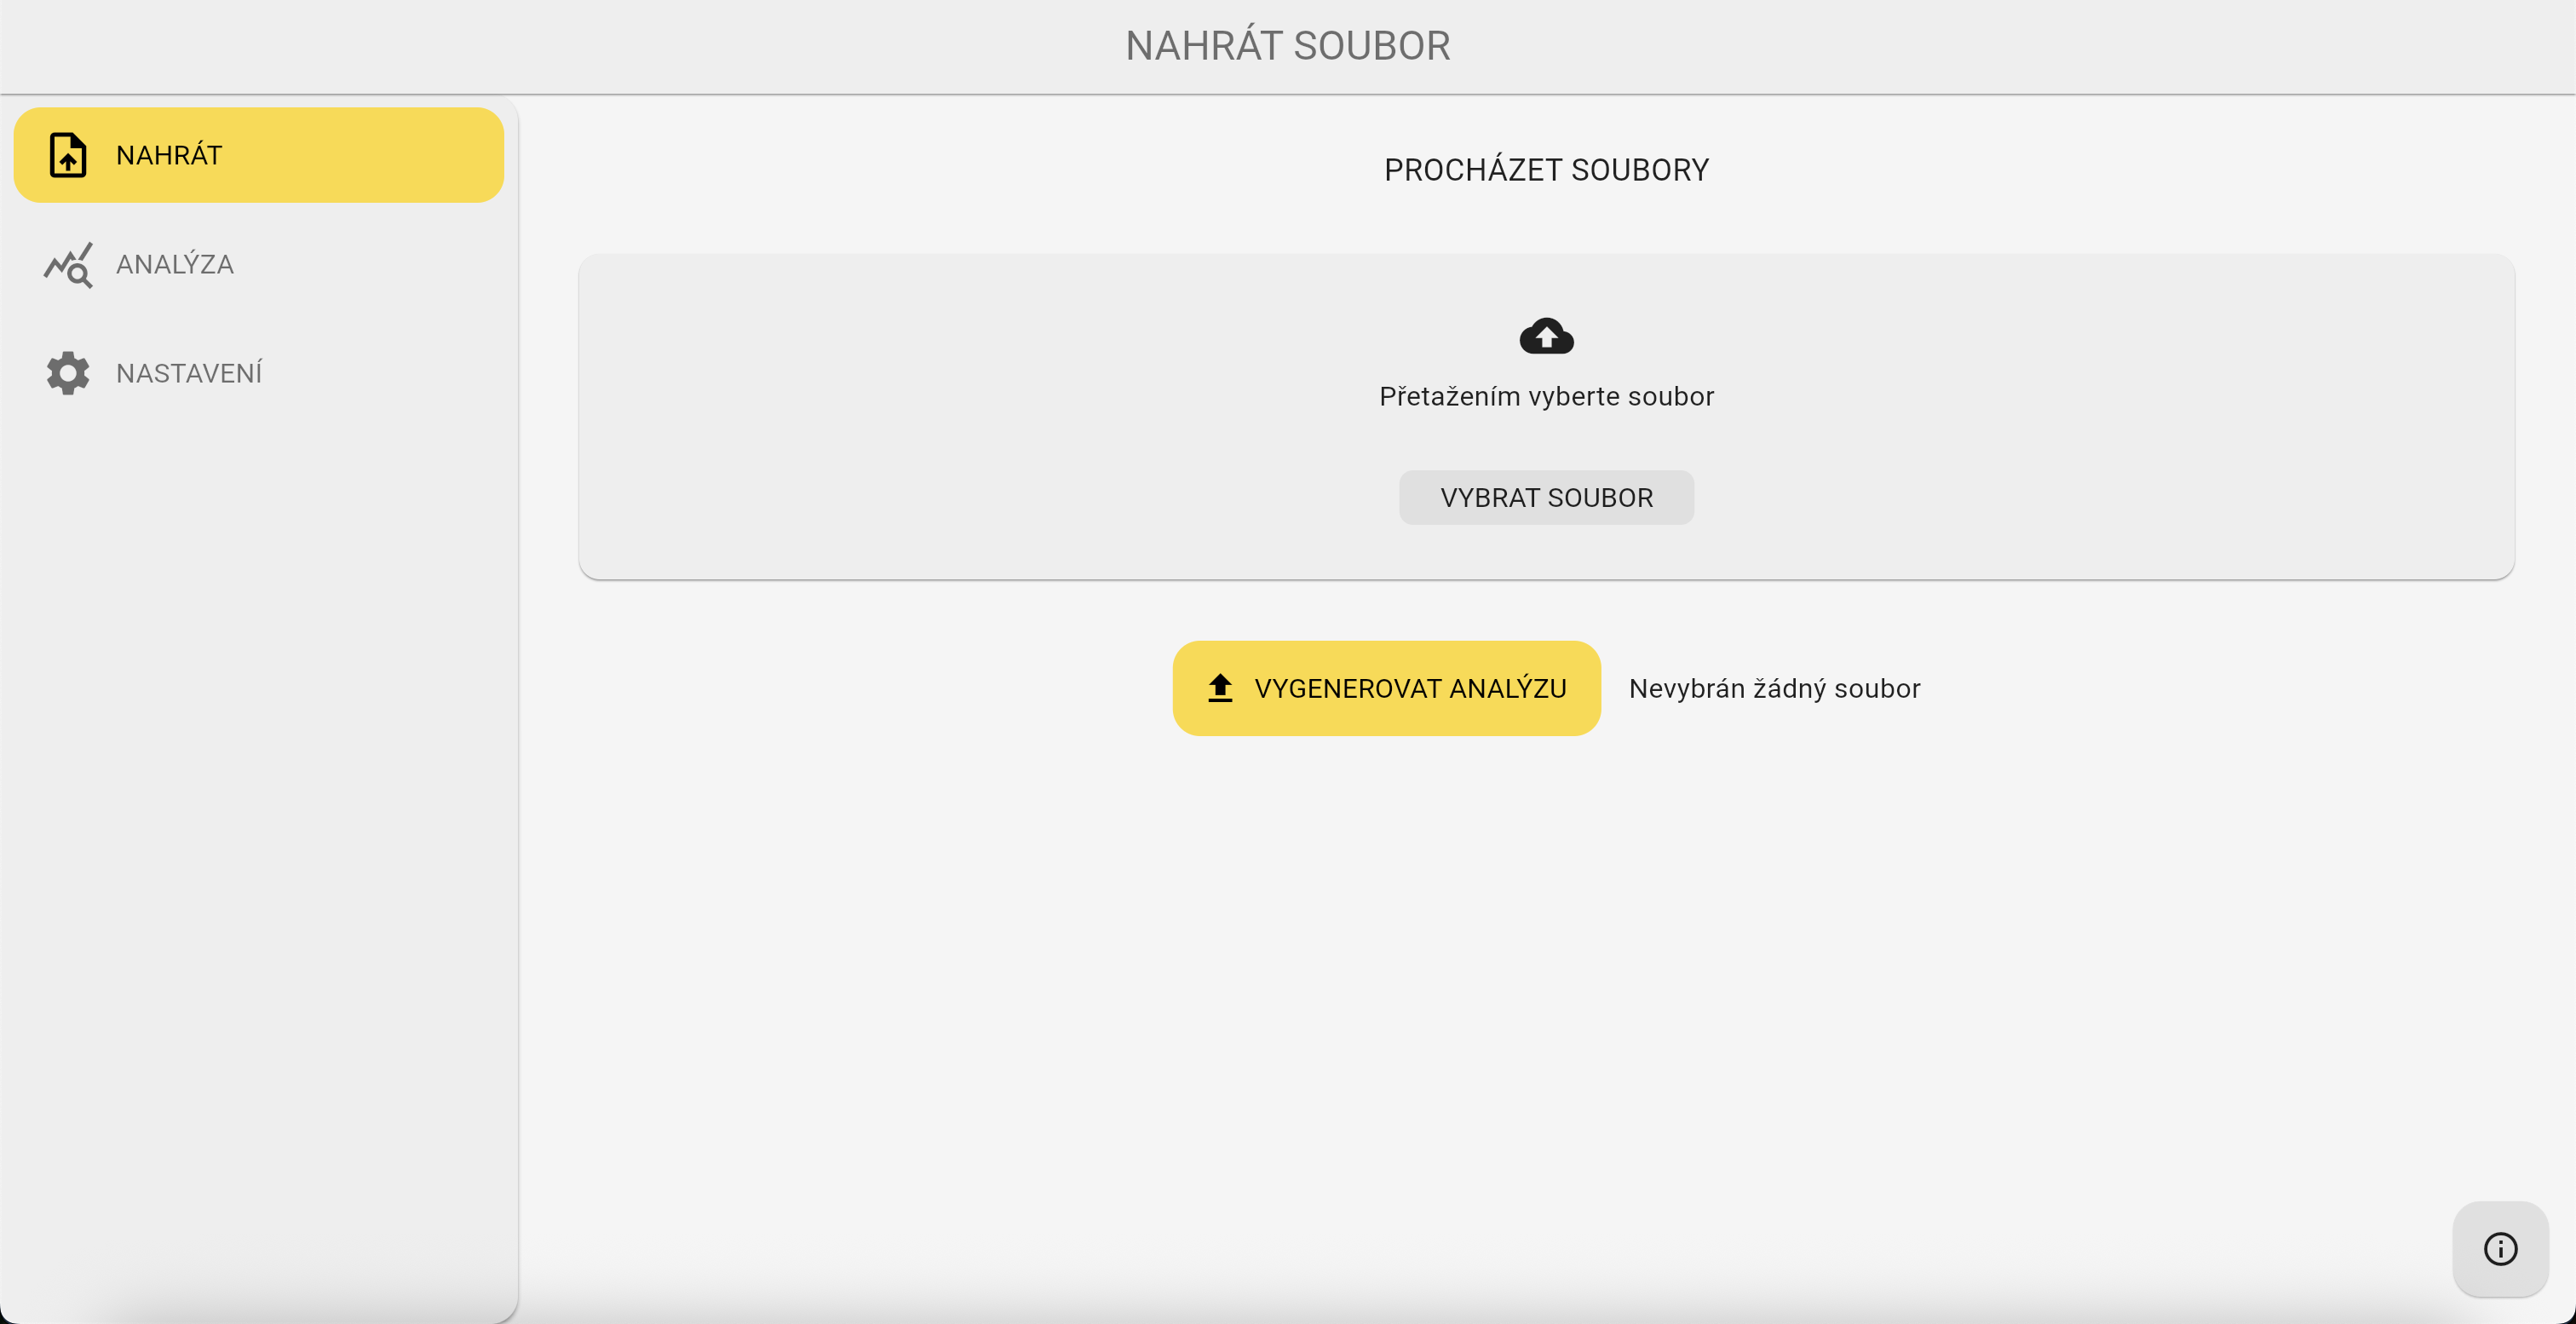
\includegraphics[width=\textwidth]{obrazky/default-screen.png}
    \caption[]{\textbf{Základní uživatelské rozhraní.} Vzhled úvodní obrazovky aplikace s~navigačním menu na levé straně a~možností výběru geografického souboru gestem přetažení do vyznačené oblasti, nebo klasickým stisknutím odpovídajícího tlačítka.}
    \label{DefaultScreen}
\end{figure}

Po výběru souboru je automaticky zkontrolována jeho přípona a~uživatel je informován o~stavu provedené akce.
Následuje konstrukce požadavku HTTP \texttt{multipart/form-data}, přičemž spolu se samotným souborem jsou na server odeslány i~doplňující parametry nastavení, mezi které se řadí například zvolené jednotky nebo minimální obtížnost náročných segmentů stoupání.
Součástí této fáze je uživatelská zpětná vazba, která během nahrávání vstupních dat zobrazuje indikátor průběhu a~po úspěšném přenosu se aplikace automaticky přesune na další obrazovku s~poskytnutými výstupy.
Nepodporované formáty vstupních dat, neplatný obsah souboru, absence výškových dat a~další chybové stavy jsou zachyceny a~zobrazeny jako hlášení s~možností opakování tohoto procesu.

Na straně serveru je vytvořen koncový bod přijímající soubor typu \texttt{UploadFile}.
Nejprve je provedena kontrola typu internetového média MIME a~validita datového obsahu.
Server dokáže rozpoznat, zda se jedná o~standardní formát a~podle toho zvolí vhodný analyzátor.
Zpracování souborů GPX probíhá s~využitím specializované knihovny \texttt{gpxpy}, soubory KML jsou načítány jako dokumenty XML, přičemž se extrahují zeměpisné souřadnice a~nadmořské výšky, a~pro soubory FIT a~TCX jsou využity dekódovací nástroje specifické pro sportovní záznamová zařízení.

Po úspěšném načtení vstupních geografických dat je provedena validace.
Ověřuje se minimální počet zaznamenaných GPS bodů, přítomnost zeměpisných souřadnic a~výškových údajů.
Pokud je některý z~předchozích požadavků nesplněn, analýza je přerušena a~klientovi se odesílá chybová zpráva.
V~opačném případě jsou data převedena do interní reprezentace, tj. seznamu bodů s~veškerými dostupnými informacemi, které jsou dále používány k~výpočtům pokročilých statistik a~generování výškových profilů.

\subsection{Nastavení aplikace a~parametrů vizualizace}
\label{setting-application-and-visualization-parameters}

Uživatelské nastavení tvoří důležitou součást celé aplikace, neboť umožňuje přizpůsobení chování nástroje a~způsobu vizualizace individuálním potřebám uživatelů.
Konfigurovatelné parametry zahrnují nejen zobrazované jednotky, konkrétně metrické, nebo imperiální, ale také volbu požadované průměrné rychlosti pro výpočty odhadovaného času jízdy na kole nebo prahu minimální obtížnosti, která slouží k~identifikaci náročných pasáží stoupání.
Uvedené hodnoty mají přímý dopad na statistické výstupy i~způsob, jakým jsou prezentovány grafické vizualizace.

Všechny tyto parametry jsou na klientské straně spravovány pomocí centrálních správců stavu implementovaných v~rámci tříd \texttt{TripProvider} a~\texttt{UnitsProvider}, které uchovávají aktuální konfiguraci v~paměti aplikace.
Využití těchto poskytovatelů, jako tzv. oznamovatelů změn, umožňuje okamžitý přístup k~nastavení a~jakákoliv změna vyvolá zprávu u~všech závislých komponent, které se automaticky překreslí dle nových hodnot.

Samotné uživatelské rozhraní pro správu nastavení je implementováno jako samostatná obrazovka, přístupná z~hlavního navigačního menu.
Její vzhled odpovídá principům responzivního designu --~na menších zařízeních je zobrazena ve formě vertikálního seznamu s~jednotlivými položkami, zatímco na větších obrazovkách jsou odpovídající skupiny nastavení rozděleny do postranních panelů.
Každý prvek rozhraní je navázán na konkrétní hodnotu poskytovatele, přičemž změny se promítají ihned do celkové konfigurace aplikace.

Uložená nastavení se při odesílání dat na server přikládají k~požadavku HTTP v~podobě běžných parametrů.
Například parametry průměrné rychlosti či použitých jednotek jsou následně využity při výpočtech na straně serveru a~k~pozdějšímu formátování výstupních statistik.

Kromě číselných a~výběrových vstupů zahrnuje nastavení i~logické přepínače, které slouží k~výběru vzhledu celé aplikace, výchozí mód však vždy odpovídá danému zařízení.
Veškerá nastavení jsou uchována pouze v~paměti aplikace po celou dobu jejího běhu, avšak v~budoucnu je plánováno rozšíření o~lokální persistenci.
Tento přístup umožní automatické načtení uživatelského nastavení při opětovném spuštění aplikace a~zvýší tak komfort při používání.

\subsection{Generování grafických výstupů}
\label{generating-graphical-output}

Vývoj multiplatformní aplikace směřuje k~vytvoření komplexního nástroje pro generování výškových profilů naplánovaných cyklistických výjezdů, které uživatelům poskytují důležité informace o~charakteru terénu.
Výstupy aplikace slouží jak pro zobrazení krátkých a~náročných úseků stoupání, tak i~pro analýzu průběhu namdořských výšek v~rámci celých tras.
I~přesto, že obě funkcionality využívají podobný výpočetní a~vizualizační základ, jejich účel a~některé klíčové detaily implementace se mírně liší.

Pro obě varianty výstupu je společná strategie založena na výběru podmnožiny dat z~GPS záznamů, respektive datových rámců, obsahujících naplánované trasy, následné normalizaci vzdáleností stanovených pomocí metody \texttt{haversine} ze sekce \ref{calculation-of-total-activity-distances-and-climb-sections} a~interpolaci hodnot nadmořských výšek.
Na základě takto předpřipravených vstupních geografických dat jsou generovány výškové profily představující přehledné grafy, které zobrazují okamžité změny nadmořských výšek v~závislosti na uražené vzdálenosti.

Vizualizace náročných úseků stoupání jsou rozděleny do určitého počtu rovnoměrných segmentů, pro které je vždy určen sklon mezi dvěma sousedními body.
Takto stanovený průměrný sklon stoupání je převeden do barevného spektra, které sahá od bílé barvy pro záporné a~nulové sklony až po tmavě červenou barvu pro extrémně prudká stoupání převyšující 18\,\%.
Díky tomu jsou uživatelé již na první pohled schopni vizuálně odlišit rovinaté úseky od náročnějších pasáží.

Izolované segmenty tras, které jsou identifikovány jako samostatná stoupání, jsou interpretovány adekvátními grafickými výstupy.
Typicky se jedná o~kratší úseky o~délce několika set metrů až jednotek kilometrů.
Grafy těchto stoupání jsou vykreslovány s~maximálním důrazem na detail, přičemž důležitou roli hrají především krátkodobé změny sklonu.
Jedním ze specifických rysů této implementace je doplňkové vyhodnocení průměrných sklonů pro dílčí délku úseků.
Tyto hodnoty a~jejich rozsahy v~rámci stoupání jsou vizualizovány pomocí horizontálních obdélníků umístěných pod samotnými výškovými profily, které reprezentují nejstrmější části v~různých stupnicích.
Tyto vícerozměrné analýzy sklonu jsou užitečné zejména při plánování tréninků různé intenzity a~lokalizaci kritických bodů trasy.

Generování průběhu celých cyklistických výjezdů sleduje pro změnu jiný účel.
Nejedná se tedy o~analýzu konkrétních stoupání, ale o~komplexní přehled.
Primárním cílem těchto výstupů je zobrazení celkové obtížnosti, rozložení jednotlivých stoupání a~klesání v~prostoru, jak ilustruje obrázek \ref{ElevationProfile}.
V~tomto kontextu není důležité detailní rozlišení úseků, nýbrž použití vhodného měřítka pro vykreslování nejen krátkých, ale rovněž maratonských výjezdů s~ohledem na celkové převýšení.

\begin{figure}[ht]
    \centering
    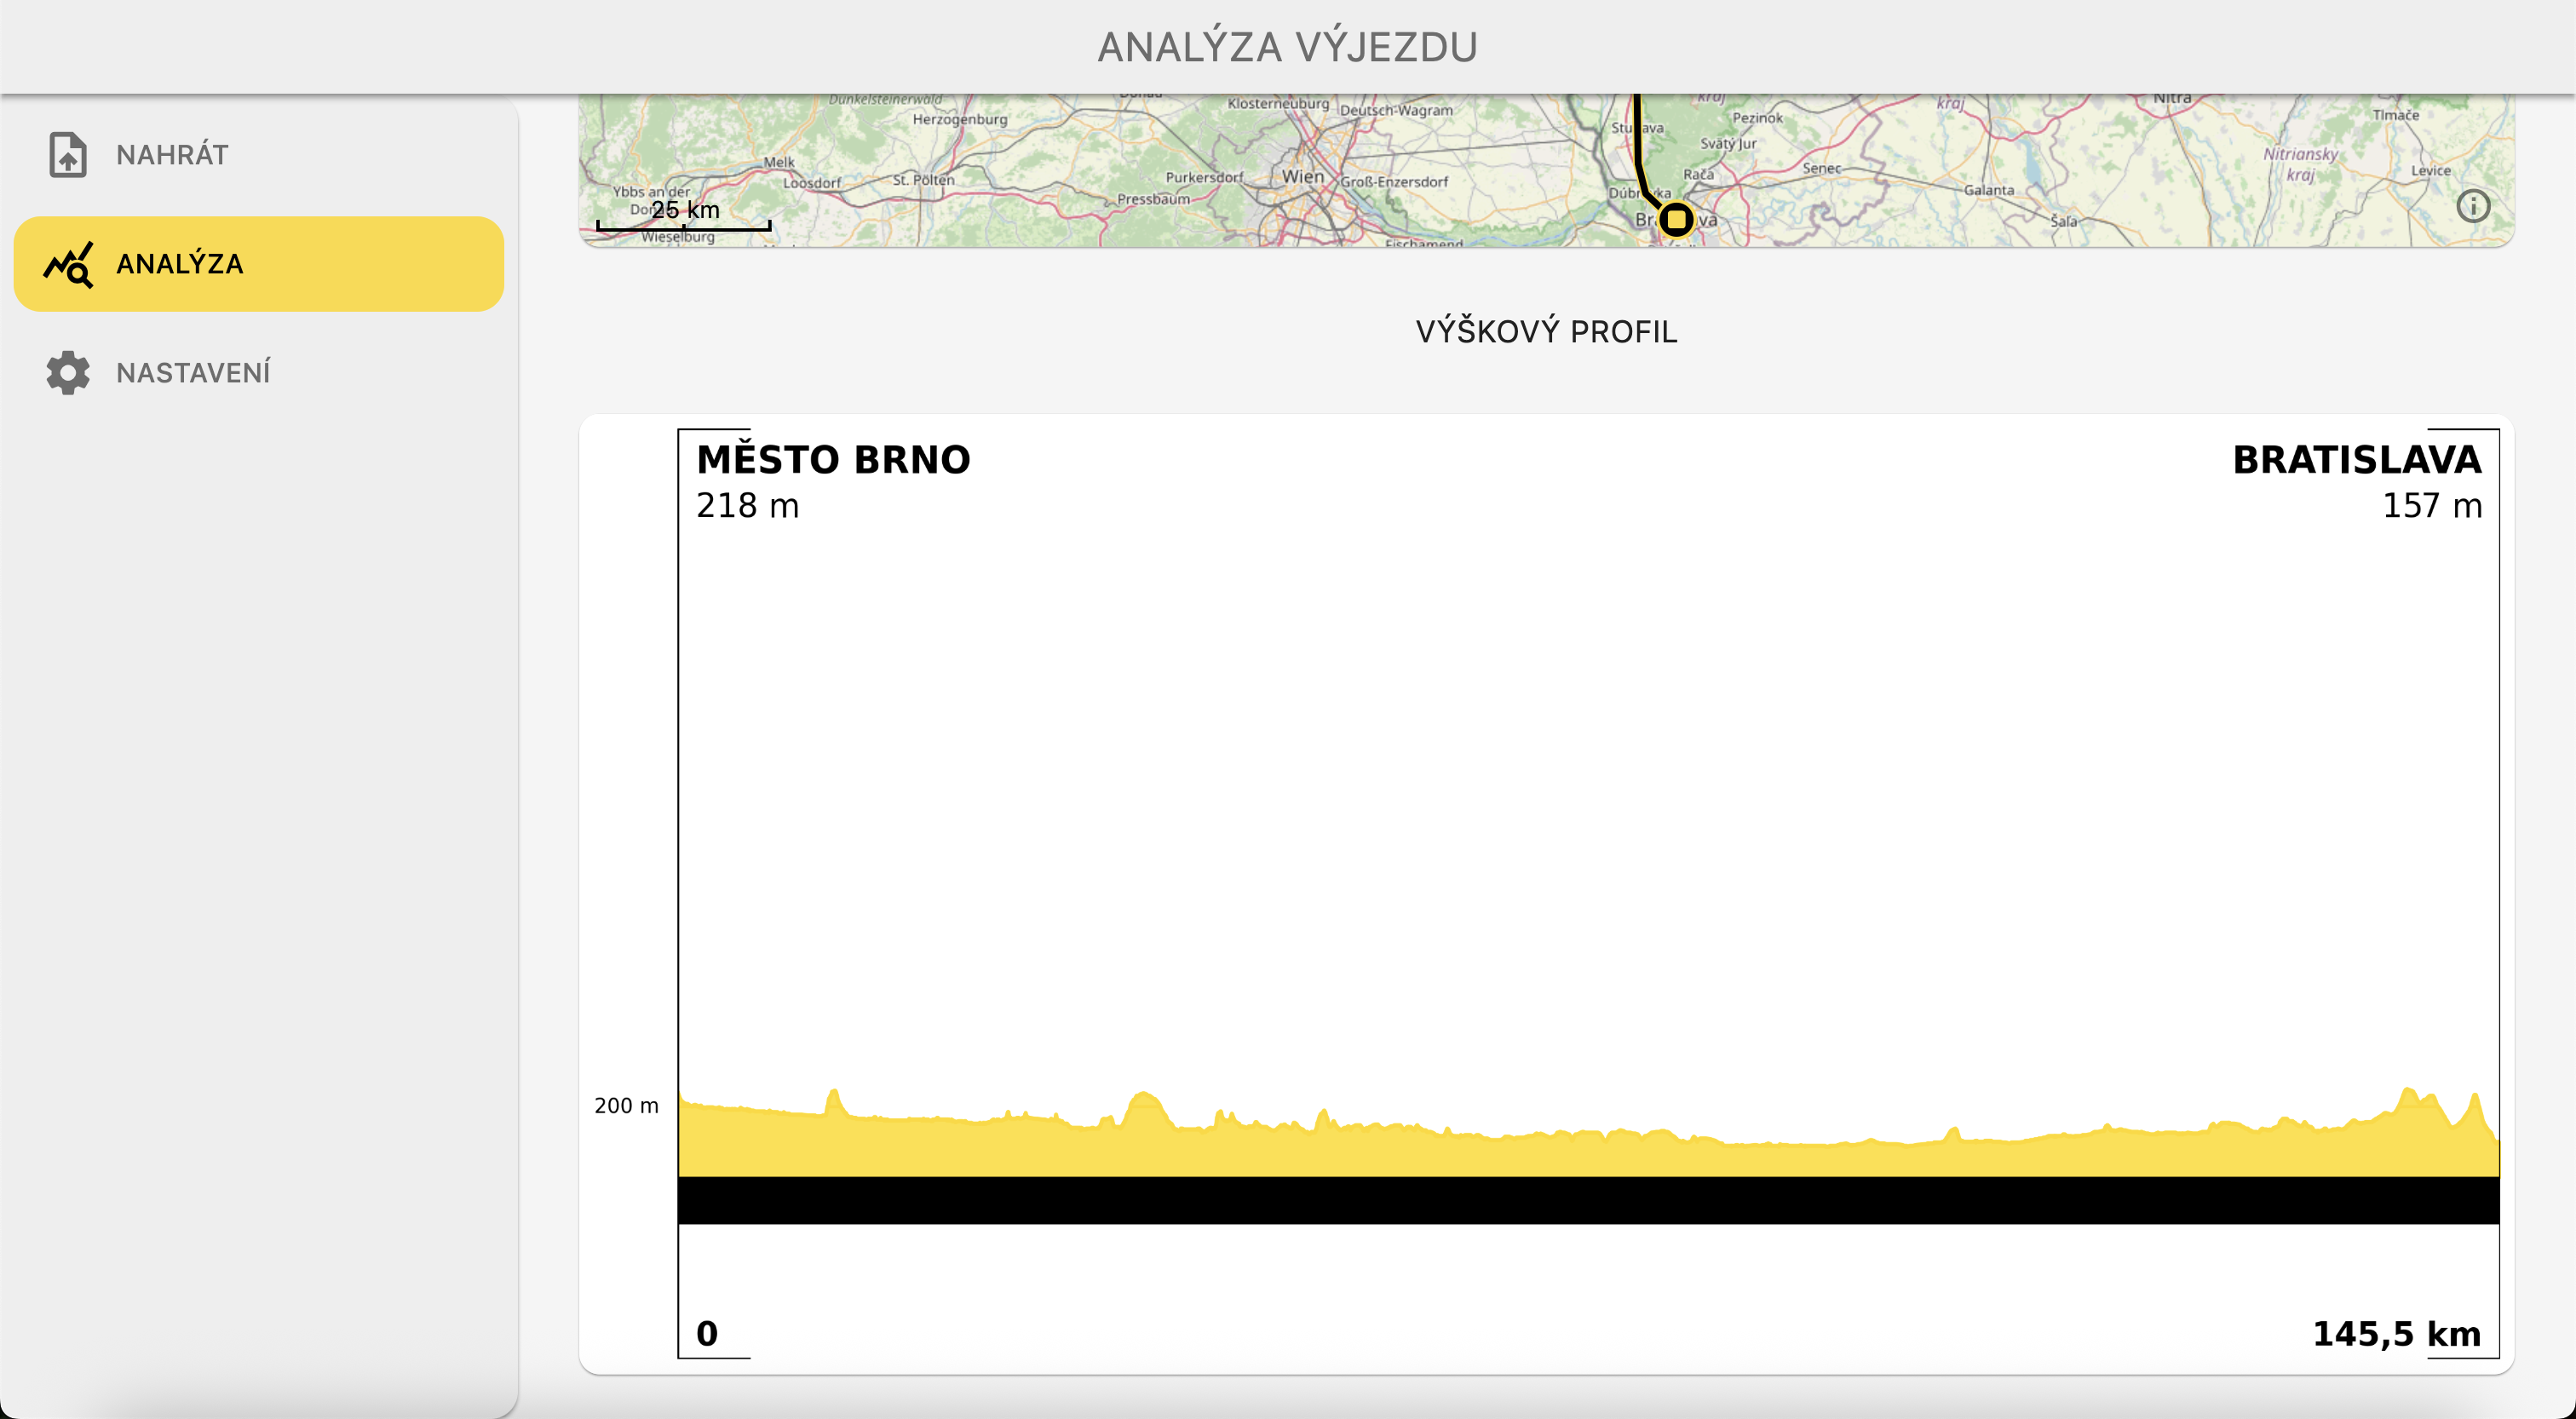
\includegraphics[width=\textwidth]{obrazky/elevation-profile.png}
    \caption[]{\textbf{Vizualizace naplánovaného cyklistického výjezdu.} Analýza cyklotras zahrnuje grafické výstupy v~podobě výškových profilů, které obsahují nejen vykreslená výšková data, ale také informace o~počátečním a~koncovém místě.}
    \label{ElevationProfile}
\end{figure}

\chapter{Testování}
\label{testing}

Fáze testování realizovaného řešení představuje klíčový krok vývoje sloužící k~ověření funkčnosti, stability a~využitelnosti aplikace.
Testování probíhalo systematicky již od samotného počátku po celou dobu implementace, přičemž využita byla výhradně reálná geografická data reprezentující naplánované cyklistické výjezdy.
Podstatou testování jsou pokročilé kontroly vstupních souborů různých formátů a~vzhled výsledných grafických vizualizací při různých připadech užití.
Součástí tohoto procesu je rovněž testování na vybrané skupině potenciálních uživatelů a~řešení poskytnutých podnětů včetně odhalených problémů.

\section{Testování různých formátů vstupního souboru}
\label{testing-different-input-file-formats}

Aplikace je navržena tak, aby podporovala vstupní data z~různých zdrojů, především ve formátech FIT, GPX, KML a~TCX, které jsou běžně využívány v~oblasti cyklistiky, sportovních a~dalších outdoorových aktivit.
Každý z~těchto formátů má své specifické vlastnosti, může obsahovat základní i~velmi podrobné údaje a~metadata.
Cílem bylo zjistit, zda je možné generovat stejné, nebo alespoň značně podobné výstupy pro naplánované cyklotrasy pomocí těchto formátů a~současně odhalit případný neplatný obsah poškozených vstupních souborů.

Průběh testování zahrnuje načítání a~zpracování dat z~reálných souborů exportovaných z~různých typů zařízení, včetně cyklopočítačů značek Garmin, Wahoo a~aplikací Strava nebo Mapy.cz.
Během testování bylo ověřeno, že implementovaný nástroj správně detekuje klíčové atributy každého záznamu a~v~případě stejných itinerářů naplánovaných výjezdů generuje grafické vizualizace s~akceptovatelnými rozdíly.

Na základě provedených testů bylo rovněž potvrzeno, že aplikace je schopna konzistentně pracovat s~uvedenými formáty a~poskytuje očekávané výsledky bez nutnosti manuálního zásahu uživatelů.
Výsledky testování ukázaly, že systém dokáže upozornit na kritické nedostatky vstupních dat, a~to prostřednictvím chybových hlášení, aniž by došlo k~neočekávanému ukončení běhu nástroje.

\section{Testování vzhledu grafických vizualizací}
\label{testing-the-appearance-of-graphical-visualizations}

Dalším významným aspektem testování je ověření korektního vykreslení grafických vizualizací, které tvoří klíčovou výstupní část aplikace, a~to jak pro celé naplánované trasy, tak i~pro dílčí výškové profily vybraných náročných úseků stoupání.
Byla zkoumána nejen technická správnost jednotlivých prvků, jako například umístění textových popisků, rozměry segmentů, barevných palet, ale také celková srozumitelnost a~estetická hodnota výsledných grafů.

Testování probíhalo na široké škále výjezdů různé vzdálenosti, profilu i~obtížnosti, přičemž byly pozorovány rozdíly v~generování výstupních vizualizací pro samostatné pasáže stoupání oproti celkovým trasám, což lze dokumentovat obrázkem \ref{Profiles}.
Zatímco u~kratších náročných stoupání hraje rozhodující roli detailní znázornění sklonu v~jednotlivých úsecích, u~delších výjezdů se klade důraz na čitelnost celkového průběhu a~přehledné označení významných bodů.
V~obou případech bylo ověřeno, že výsledné grafy zachovávají jednotný vizuální styl a~jsou schopné se adaptovat v~závislosti na vlastnostech a~celkové vzdálenosti aktivity.

Nedílnou součástí testovacích scénářů je i~kontrola výstupů při odlišných jazykových lokalizacích, stejně jako použitých měrných jednotkách, kdy je nutné zajistit adekvátní formátování číselných hodnot a~textových popisků, včetně přepočtů mezi metrickými a~imperiálními jednotkami.
Výsledky testování ukázaly, že implementovaný nástroj dokáže spolehlivě reflektovat volbu uživatelů bez narušení struktury vygenerovaných grafů.
Na obrázku \ref{ProfileSettings} lze pozorovat vzhled výškových profilů při nastavení imperiálních jednotek.

\begin{figure}[ht]
    \centering
    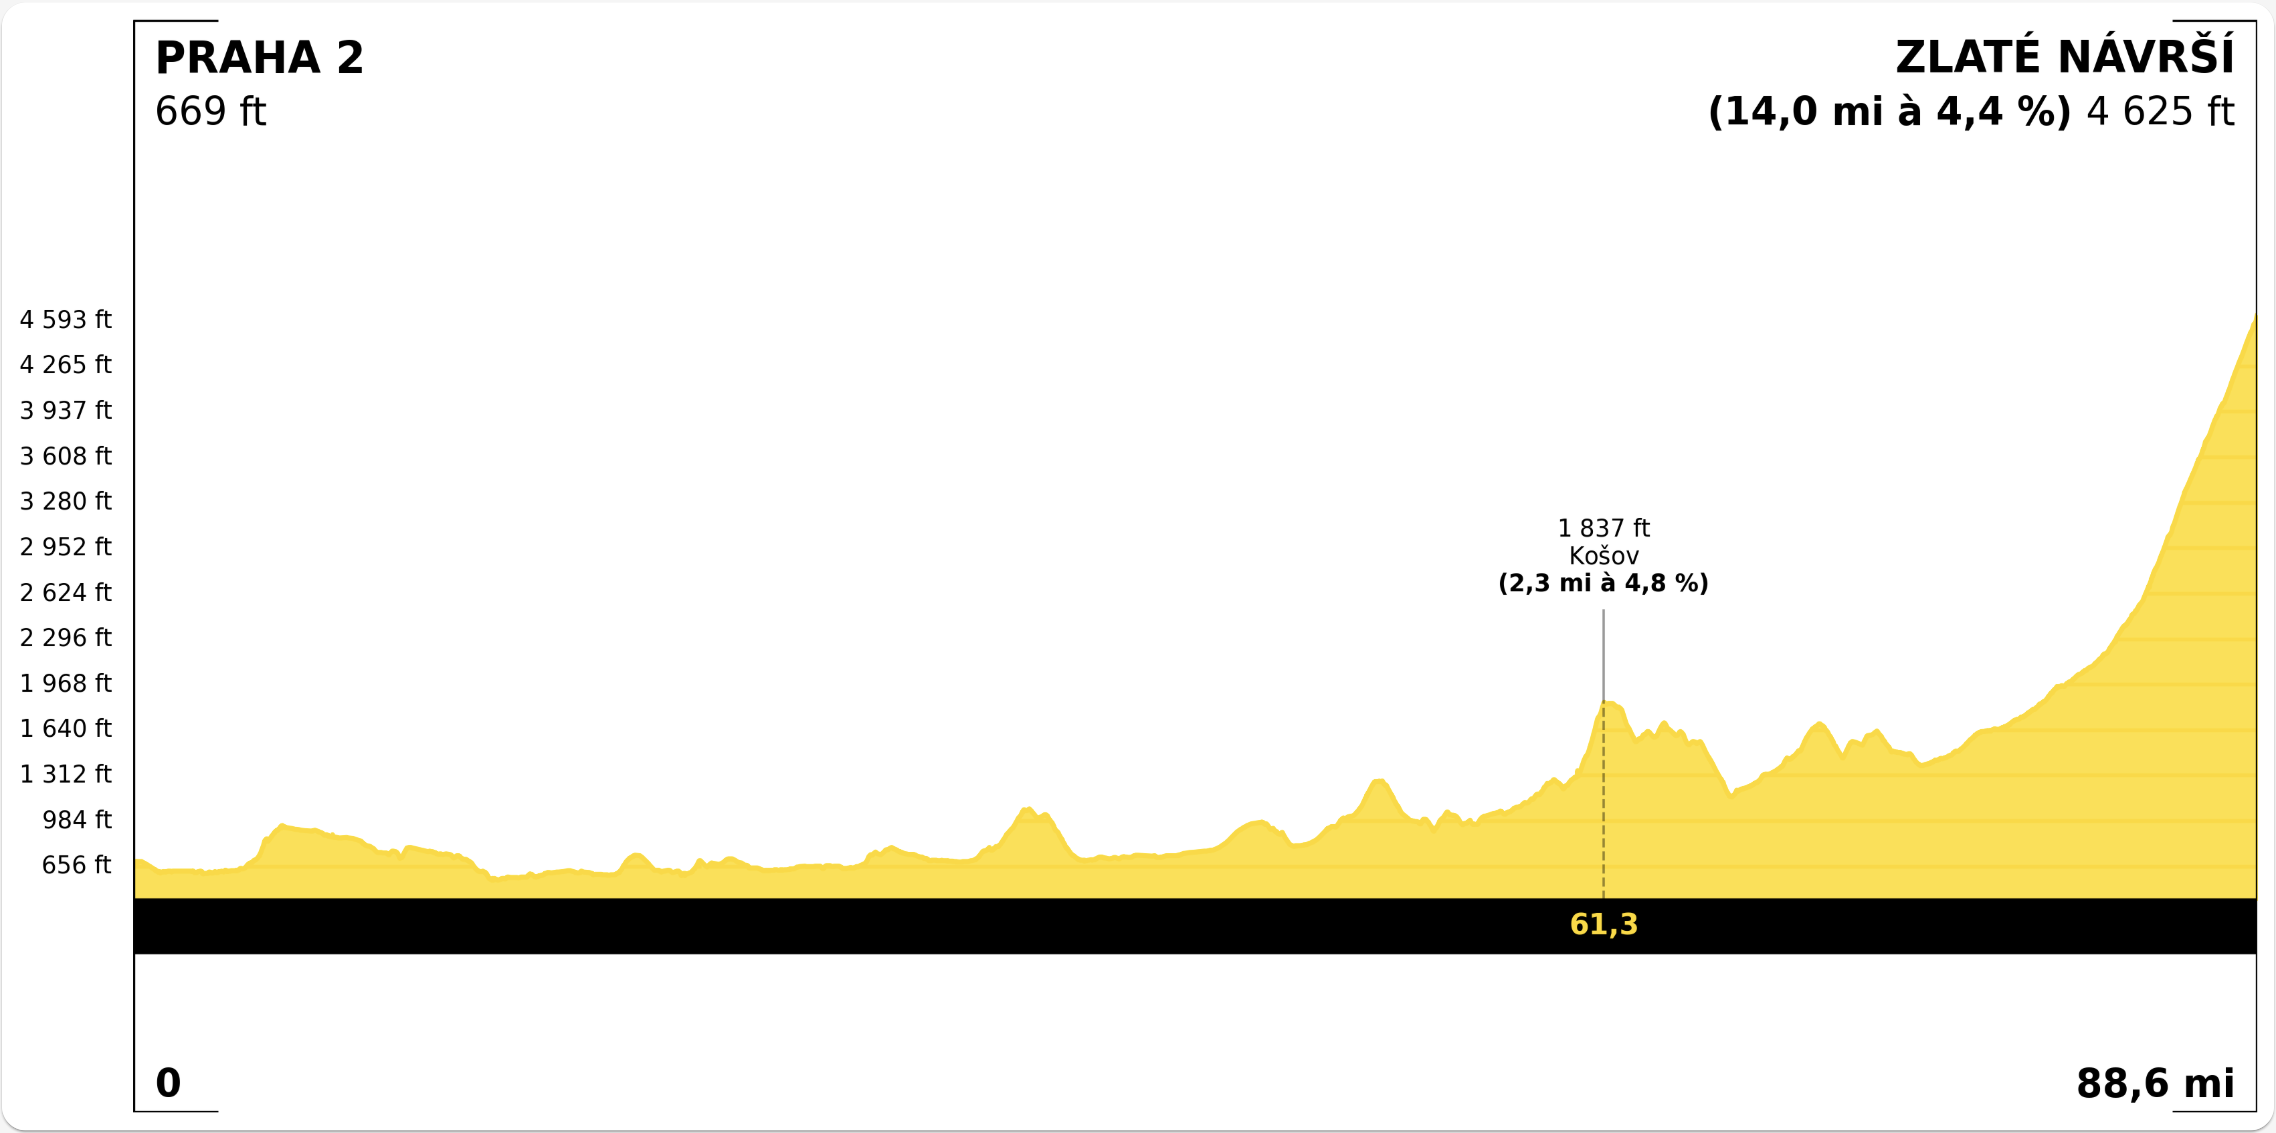
\includegraphics[width=\textwidth]{obrazky/profile-settings.png}
    \caption[]{\textbf{Uživatelské nastavení grafické vizualizace.} Při změně nastavení měrných jednotek nedochází ke zkreslení grafu ani převodu použitého měřítka, ale pouze k~odpovídající úpravě textových popisků.}
    \label{ProfileSettings}
\end{figure}

\section{Řešení odhalených problémů}
\label{solving-detected-problems}

Proces testování systematicky doplňoval celou fázi implementace.
Mnoho chyb a~nedostatků se podařilo odhalit a~následně opravit průběžně, včetně technických problémů týkajících se načítání souborů, práce s~chybějícími daty či stability výstupů.
Závěrečná etapa testování, do které byli zapojeni také potenciální uživatelé, však přinesla několik podnětů a~ukázala nedostatky, které vyžadovaly cílené úpravy.
Jedním z~těchto problémů byla chybějící možnost přepínání mezi metrickými a~imperiálními jednotkami, což omezovalo využitelnost aplikace v~mezinárodním kontextu.
Tento nedostatek byl na základě zpětné vazby odstraněn přidáním volitelného nastavení jednotek, které se následně promítá jak do textového výstupu statistik, tak do grafických vizualizací.

Dalším zjištěným omezením byla realizace reverzního geokódování, původně zamýšlená pro automatické určování názvů lokalit v~průběhu celých aktivit.
Vzhledem k~výrazné časové a~výpočetní náročnosti tohoto procesu a~k~limitacím veřejně dostupných služeb bylo přistoupeno k~omezujícímu řešení, které zahrnuje pouze identifikaci výchozího a~cílového místa a~hlavního vrcholu individuálních stoupání.

Zásadním problémem, který se během testování nepodařilo uspokojivě vyřešit, je pokročilá analýza typu povrchu, jako jednoho z~parametrů pro objektivní hodnocení obtížnosti cyklotras.
Bylo zjištěno, že dostupnost těchto dat je omezená a~značně závislá na komunitě uživatelů otevřených platforem, jako je OpenStreetMap, které nejsou v~tomto ohledu dostatečně konzistentní a~spolehlivé.
S~ohledem na tato omezení bylo rozhodnuto tento parametr z~výsledné analýzy vyloučit, přičemž zůstává perspektivním směrem pro případný budoucí vývoj.
Absence této metriky však žádným výrazným způsobem nezasahuje do vizualizace výškových profilů.

\begin{figure}[ht]
    \centering
    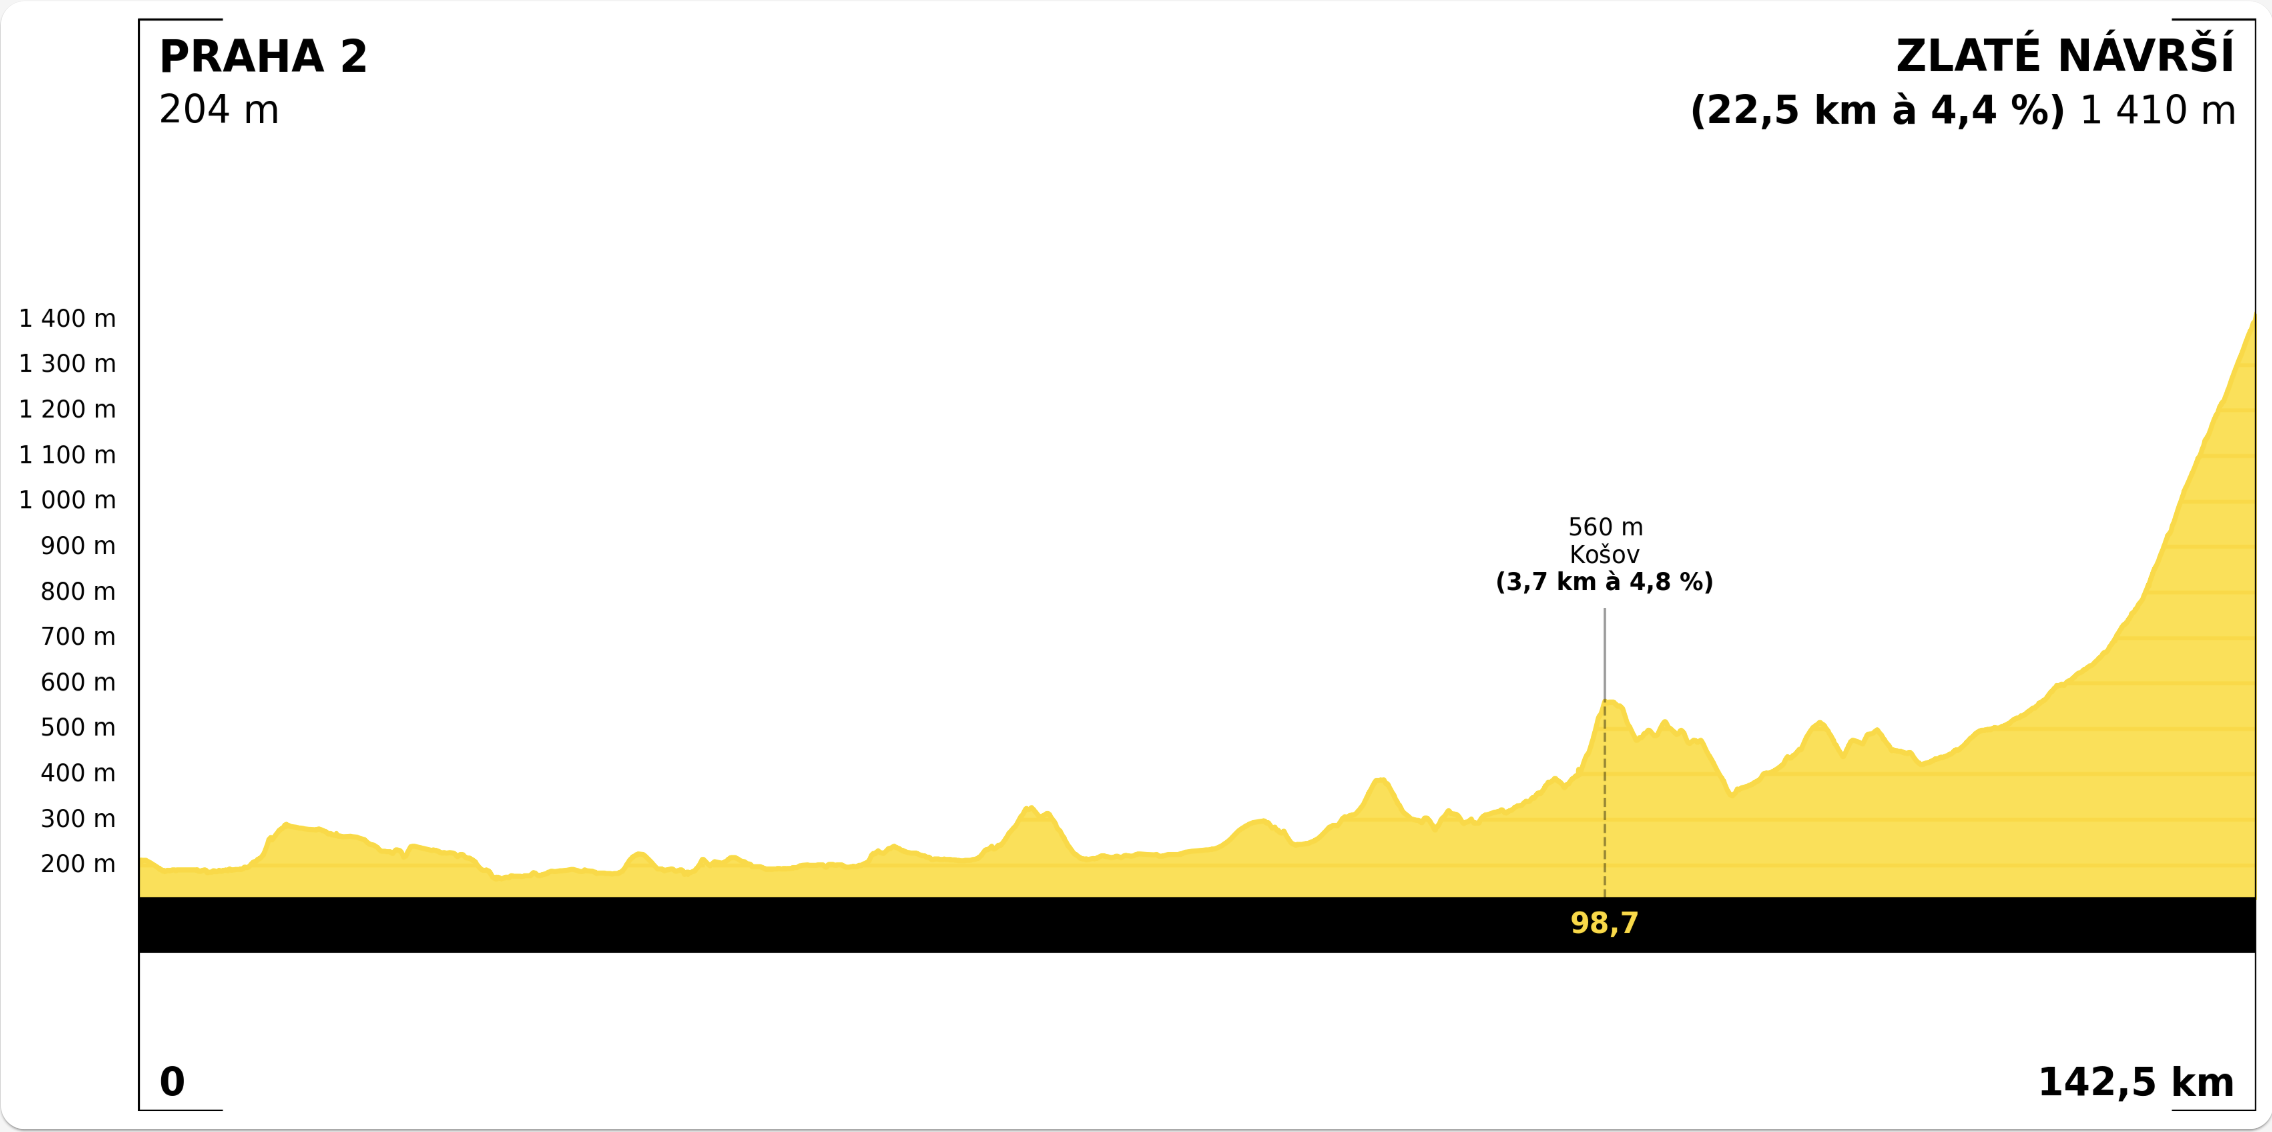
\includegraphics[width=\textwidth]{obrazky/trip-profile.png}
    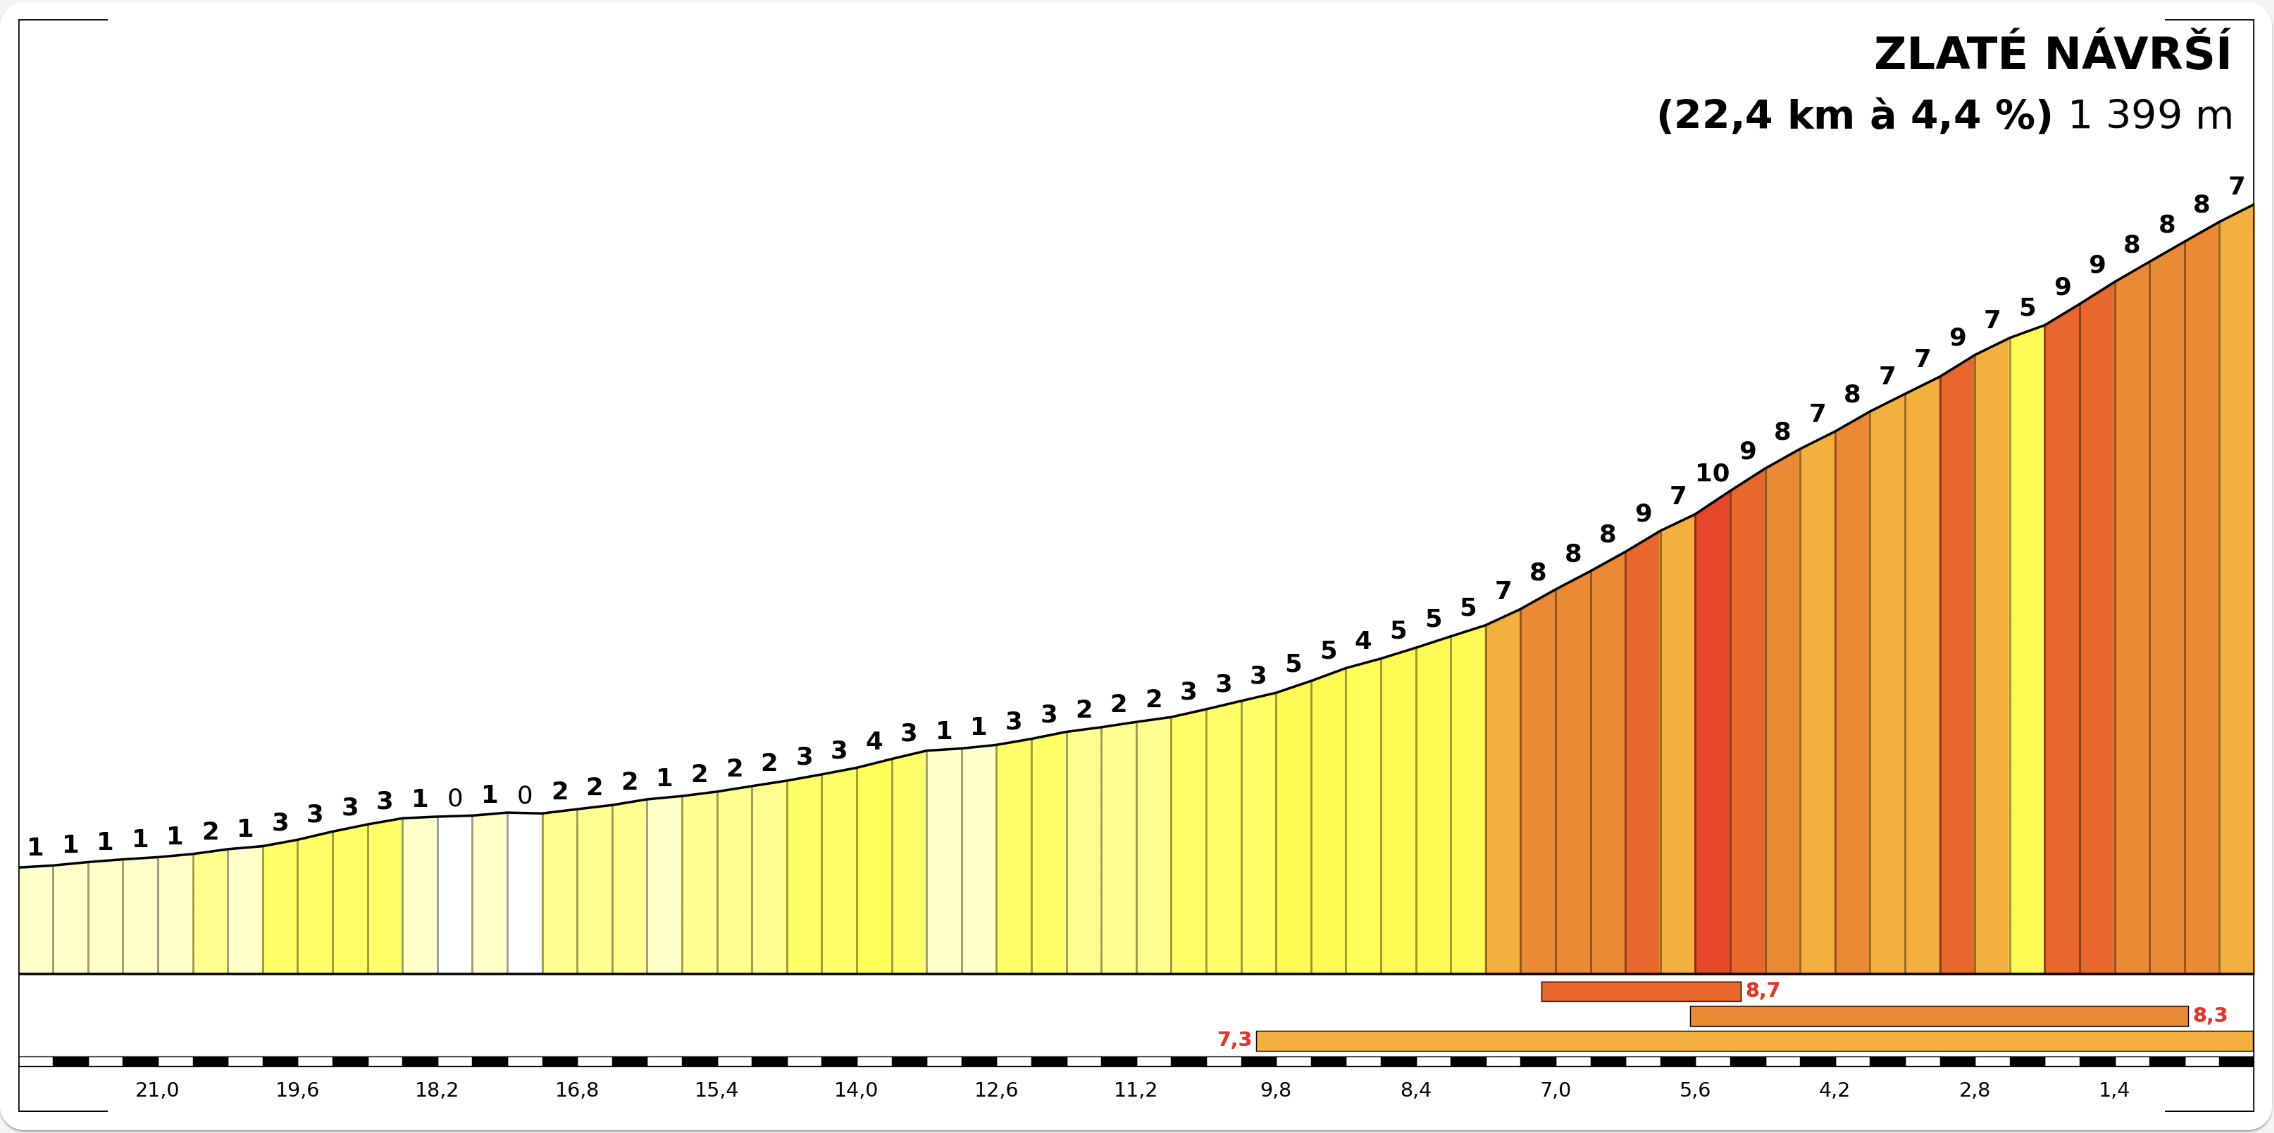
\includegraphics[width=\textwidth]{obrazky/climb-profile.png}
    \caption[]{\textbf{Porovnání výškových profilů.} Rozdíly mezi vygenerovanými výškovými profily celé naplánované trasy a~identifikovaného stoupání.}
    \label{Profiles}
\end{figure}

\chapter{Závěr}
\label{conclusion}

Cílem této práce bylo vytvořit aplikaci, která bude poskytovat detailní grafické analýzy naplánovaných cyklistických výjezdů s~důrazem na jejich objektivní hodnocení obtížnosti.
Nedílnou součástí řešení byl průzkum existujících nástrojů sloužících k~těmto účelům.
Prostudování všeobecně používaných formátů geografických dat, stejně jako různé způsoby jejich interpretace v~závislosti na konkrétním účelu, přispěly k~definování základních postupů realizace.
Na základě provedeného uživatelského průzkumu bylo možné stanovit specifické požadavky, které musí navržené řešení splňovat.

Výsledným produktem je multiplatformní aplikace, která se zaměřuje primárně na důkladné plánování cyklistických tras.
Implementovaný nástroj je schopen graficky vizualizovat přesný průběh naplánovaných výjezdů pocházejících z~reálných dat a~opticky rozlišit případy, kdy se jedná o~snadné a~rovinaté etapy v~porovnání s~náročnými kopcovitými aktivitami.
Velký důraz je kladen také na znázornění náročných úseků stoupání, která se vyskytují v~průběhu celých tras.
Omezujícím faktorem je dostupnost doplňujících informací souvisejících s~různými typy povrchu, které v~některých případech vedou ke značným nárůstům obtížnosti nejen co se týče celých cyklotras, ale také jednotlivých pasáží stoupání.

Aplikace pracuje nad specifickými datovými formáty vstupních souborů.
Možnosti budoucího rozšíření funkcionality nástroje pokrývají tuto oblast v~podobě podpory dalších standardů geografických dat.
Zároveň schopnost posuzovat obtížnosti naplánovaných cyklistických výjezdů na základě rozšířených ovlivňujících aspektů by uživatelům poskytlo nový rozměr výstupů v~rámci procesu plánování a~porovnávání tras.

V~současnosti existuje mnoho aplikací, které se zaměřují převážně na rozbor statistik již absolvovaných sportovních výkonů.
Hlavním smyslem implementovaného nástroje je usnadnit plánování aktivit podle náročnosti terénu a~detailním způsobem vizuálně zprostředkovat přesný průběh cyklistických výjezdů a~identifikovaných úseků stoupání.
Potenciál využití této aplikace spočívá v~možnosti efektivního rozvržení fyzických sil s~ohledem na objektivní obtížnosti tras, přičemž nástroj vhodně rozšiřuje portfolio stávajících řešení o~podrobný analytický pohled.
